\PassOptionsToPackage{unicode=true}{hyperref} % options for packages loaded elsewhere
\PassOptionsToPackage{hyphens}{url}
%
\documentclass[12pt,]{book}
\usepackage{lmodern}
\usepackage{amssymb,amsmath}
\usepackage{ifxetex,ifluatex}
\usepackage{fixltx2e} % provides \textsubscript
\ifnum 0\ifxetex 1\fi\ifluatex 1\fi=0 % if pdftex
  \usepackage[T1]{fontenc}
  \usepackage[utf8]{inputenc}
  \usepackage{textcomp} % provides euro and other symbols
\else % if luatex or xelatex
  \usepackage{unicode-math}
  \defaultfontfeatures{Ligatures=TeX,Scale=MatchLowercase}
    \setmonofont[Mapping=tex-ansi,Scale=0.7]{Source Code Pro}
\fi
% use upquote if available, for straight quotes in verbatim environments
\IfFileExists{upquote.sty}{\usepackage{upquote}}{}
% use microtype if available
\IfFileExists{microtype.sty}{%
\usepackage[]{microtype}
\UseMicrotypeSet[protrusion]{basicmath} % disable protrusion for tt fonts
}{}
\IfFileExists{parskip.sty}{%
\usepackage{parskip}
}{% else
\setlength{\parindent}{0pt}
\setlength{\parskip}{6pt plus 2pt minus 1pt}
}
\usepackage{hyperref}
\hypersetup{
            pdftitle={BIO4558 Biostatistiques appliquées avec R},
            pdfauthor={Julien Martin},
            pdfborder={0 0 0},
            breaklinks=true}
\urlstyle{same}  % don't use monospace font for urls
\usepackage{color}
\usepackage{fancyvrb}
\newcommand{\VerbBar}{|}
\newcommand{\VERB}{\Verb[commandchars=\\\{\}]}
\DefineVerbatimEnvironment{Highlighting}{Verbatim}{commandchars=\\\{\}}
% Add ',fontsize=\small' for more characters per line
\usepackage{framed}
\definecolor{shadecolor}{RGB}{248,248,248}
\newenvironment{Shaded}{\begin{snugshade}}{\end{snugshade}}
\newcommand{\AlertTok}[1]{\textcolor[rgb]{0.33,0.33,0.33}{#1}}
\newcommand{\AnnotationTok}[1]{\textcolor[rgb]{0.37,0.37,0.37}{\textbf{\textit{#1}}}}
\newcommand{\AttributeTok}[1]{\textcolor[rgb]{0.61,0.61,0.61}{#1}}
\newcommand{\BaseNTok}[1]{\textcolor[rgb]{0.06,0.06,0.06}{#1}}
\newcommand{\BuiltInTok}[1]{#1}
\newcommand{\CharTok}[1]{\textcolor[rgb]{0.5,0.5,0.5}{#1}}
\newcommand{\CommentTok}[1]{\textcolor[rgb]{0.37,0.37,0.37}{\textit{#1}}}
\newcommand{\CommentVarTok}[1]{\textcolor[rgb]{0.37,0.37,0.37}{\textbf{\textit{#1}}}}
\newcommand{\ConstantTok}[1]{\textcolor[rgb]{0,0,0}{#1}}
\newcommand{\ControlFlowTok}[1]{\textcolor[rgb]{0.27,0.27,0.27}{\textbf{#1}}}
\newcommand{\DataTypeTok}[1]{\textcolor[rgb]{0.27,0.27,0.27}{#1}}
\newcommand{\DecValTok}[1]{\textcolor[rgb]{0.06,0.06,0.06}{#1}}
\newcommand{\DocumentationTok}[1]{\textcolor[rgb]{0.37,0.37,0.37}{\textbf{\textit{#1}}}}
\newcommand{\ErrorTok}[1]{\textcolor[rgb]{0.14,0.14,0.14}{\textbf{#1}}}
\newcommand{\ExtensionTok}[1]{#1}
\newcommand{\FloatTok}[1]{\textcolor[rgb]{0.06,0.06,0.06}{#1}}
\newcommand{\FunctionTok}[1]{\textcolor[rgb]{0,0,0}{#1}}
\newcommand{\ImportTok}[1]{#1}
\newcommand{\InformationTok}[1]{\textcolor[rgb]{0.37,0.37,0.37}{\textbf{\textit{#1}}}}
\newcommand{\KeywordTok}[1]{\textcolor[rgb]{0.27,0.27,0.27}{\textbf{#1}}}
\newcommand{\NormalTok}[1]{#1}
\newcommand{\OperatorTok}[1]{\textcolor[rgb]{0.43,0.43,0.43}{\textbf{#1}}}
\newcommand{\OtherTok}[1]{\textcolor[rgb]{0.37,0.37,0.37}{#1}}
\newcommand{\PreprocessorTok}[1]{\textcolor[rgb]{0.37,0.37,0.37}{\textit{#1}}}
\newcommand{\RegionMarkerTok}[1]{#1}
\newcommand{\SpecialCharTok}[1]{\textcolor[rgb]{0,0,0}{#1}}
\newcommand{\SpecialStringTok}[1]{\textcolor[rgb]{0.5,0.5,0.5}{#1}}
\newcommand{\StringTok}[1]{\textcolor[rgb]{0.5,0.5,0.5}{#1}}
\newcommand{\VariableTok}[1]{\textcolor[rgb]{0,0,0}{#1}}
\newcommand{\VerbatimStringTok}[1]{\textcolor[rgb]{0.5,0.5,0.5}{#1}}
\newcommand{\WarningTok}[1]{\textcolor[rgb]{0.37,0.37,0.37}{\textbf{\textit{#1}}}}
\usepackage{longtable,booktabs}
% Fix footnotes in tables (requires footnote package)
\IfFileExists{footnote.sty}{\usepackage{footnote}\makesavenoteenv{longtable}}{}
\usepackage{graphicx,grffile}
\makeatletter
\def\maxwidth{\ifdim\Gin@nat@width>\linewidth\linewidth\else\Gin@nat@width\fi}
\def\maxheight{\ifdim\Gin@nat@height>\textheight\textheight\else\Gin@nat@height\fi}
\makeatother
% Scale images if necessary, so that they will not overflow the page
% margins by default, and it is still possible to overwrite the defaults
% using explicit options in \includegraphics[width, height, ...]{}
\setkeys{Gin}{width=\maxwidth,height=\maxheight,keepaspectratio}
\setlength{\emergencystretch}{3em}  % prevent overfull lines
\providecommand{\tightlist}{%
  \setlength{\itemsep}{0pt}\setlength{\parskip}{0pt}}
\setcounter{secnumdepth}{5}
% Redefines (sub)paragraphs to behave more like sections
\ifx\paragraph\undefined\else
\let\oldparagraph\paragraph
\renewcommand{\paragraph}[1]{\oldparagraph{#1}\mbox{}}
\fi
\ifx\subparagraph\undefined\else
\let\oldsubparagraph\subparagraph
\renewcommand{\subparagraph}[1]{\oldsubparagraph{#1}\mbox{}}
\fi

% set default figure placement to htbp
\makeatletter
\def\fps@figure{htbp}
\makeatother

\usepackage{booktabs}
\usepackage{longtable}
\usepackage[bf,singlelinecheck=off]{caption}
\usepackage{sourcecodepro}
%\usepackage{Alegreya}

\setmainfont[UprightFeatures={SmallCapsFont=AlegreyaSC-Regular}]{Alegreya}

\usepackage{framed,color}
\definecolor{shadecolor}{RGB}{248,248,248}

\renewcommand{\textfraction}{0.05}
\renewcommand{\topfraction}{0.8}
\renewcommand{\bottomfraction}{0.8}
\renewcommand{\floatpagefraction}{0.75}

%\renewenvironment{quote}{\begin{VF}}{\end{VF}}

\let\oldhref\href
\renewcommand{\href}[2]{#2\footnote{\url{#1}}}

\ifxetex
  \usepackage{letltxmacro}
  \setlength{\XeTeXLinkMargin}{1pt}
  \LetLtxMacro\SavedIncludeGraphics\includegraphics
  \def\includegraphics#1#{% #1 catches optional stuff (star/opt. arg.)
    \IncludeGraphicsAux{#1}%
  }%
  \newcommand*{\IncludeGraphicsAux}[2]{%
    \XeTeXLinkBox{%
      \SavedIncludeGraphics#1{#2}%
    }%
  }%
\fi

\makeatletter
\newenvironment{kframe}{%
\medskip{}
\setlength{\fboxsep}{.8em}
 \def\at@end@of@kframe{}%
 \ifinner\ifhmode%
  \def\at@end@of@kframe{\end{minipage}}%
  \begin{minipage}{\columnwidth}%
 \fi\fi%
 \def\FrameCommand##1{\hskip\@totalleftmargin \hskip-\fboxsep
 \colorbox{shadecolor}{##1}\hskip-\fboxsep
     % There is no \\@totalrightmargin, so:
     \hskip-\linewidth \hskip-\@totalleftmargin \hskip\columnwidth}%
 \MakeFramed {\advance\hsize-\width
   \@totalleftmargin\z@ \linewidth\hsize
   \@setminipage}}%
 {\par\unskip\endMakeFramed%
 \at@end@of@kframe}
\makeatother

\makeatletter
\@ifundefined{Shaded}{
}{\renewenvironment{Shaded}{\begin{kframe}}{\end{kframe}}}
\makeatother

\newenvironment{rmdblock}[1]
  {
  \begin{itemize}
  \renewcommand{\labelitemi}{
    \raisebox{-.7\height}[0pt][0pt]{
      {\setkeys{Gin}{width=3em,keepaspectratio}\includegraphics{images/#1}}
    }
  }
  \setlength{\fboxsep}{1em}
  \begin{kframe}
  \item
  }
  {
  \end{kframe}
  \end{itemize}
  }
\newenvironment{rmdnote}
  {\begin{rmdblock}{note}}
  {\end{rmdblock}}
\newenvironment{rmdcaution}
  {\begin{rmdblock}{caution}}
  {\end{rmdblock}}
\newenvironment{rmdimportant}
  {\begin{rmdblock}{important}}
  {\end{rmdblock}}
\newenvironment{rmdtip}
  {\begin{rmdblock}{tip}}
  {\end{rmdblock}}
\newenvironment{rmdwarning}
  {\begin{rmdblock}{warning}}
  {\end{rmdblock}}
\newenvironment{rmdcode}
  {\begin{rmdblock}{screen}}
  {\end{rmdblock}}

\usepackage{makeidx}
\makeindex

\urlstyle{tt}

\usepackage{amsthm}
\makeatletter
\def\thm@space@setup{%
  \thm@preskip=8pt plus 2pt minus 4pt
  \thm@postskip=\thm@preskip
}
\makeatother

%\frontmatter
\usepackage[]{natbib}
\bibliographystyle{plainnat}

\title{BIO4558 Biostatistiques appliquées avec R}
\providecommand{\subtitle}[1]{}
\subtitle{Manuel de Laboratoire}
\author{Julien Martin}
\date{04-09-2020}

\begin{document}
\maketitle

%\cleardoublepage\newpage\thispagestyle{empty}\null
%\cleardoublepage\newpage\thispagestyle{empty}\null
%\cleardoublepage\newpage
%\thispagestyle{empty}
%\begin{center}
%
\includegraphics{images/missing.png}
%\end{center}

%\setlength{\abovedisplayskip}{-5pt}
%\setlength{\abovedisplayshortskip}{-5pt}

{
\setcounter{tocdepth}{1}
\tableofcontents
}
\hypertarget{note}{%
\chapter*{Note}\label{note}}


Version en cours de développement pour le cours de l'automne 2020. Les chapitres vont apparaitre au cours de la session.

\hypertarget{pruxe9face}{%
\chapter*{Préface}\label{pruxe9face}}


Les exercices de laboratoire que vous retrouverez dans les pages qui suivent sont conçus de manière à vous permettre de développer une expérience pratique en analyse de données à l'aide d'un logiciel (R).
R est un logiciel très puissant, mais comme tous les logiciels, il a des limites.
En particulier il ne peut réfléchir à votre place, vous dire si l'analyse que vous tentez d'effectuer est appropriée ou sensée, ou interpréter biologiquement les résultats.

\hypertarget{quelques-points-importants-uxe0-retenir}{%
\section*{Quelques points importants à retenir}\label{quelques-points-importants-uxe0-retenir}}


\begin{itemize}
\item
  Avant de commencer une analyse statistique, il faut d'abord vous familiariser son fonctionnement.
  Cela ne veut pas dire que vous devez connaître les outils mathématiques qui la sous-tendent, mais vous devriez au moins comprendre les principes utilisés lors de cette analyse.
  Avant de faire un exercice de laboratoire, lisez donc la section correspondante dans les notes de cours.
  Sans cette lecture préalable, il est très probable que les résultats produits par le logiciel, même si l'analyse a été effectuée correctement, seront indéchiffrables.
\item
  Les laboratoires sont conçus pour compléter les cours théoriques et vice versa.
  À cause des contraintes d'horaires, il se pourrait que le cours et le laboratoire ne soient pas parfaitement synchronisés.
  N'hésitez donc pas à poser des questions sur le labo en classe ou des questions théoriques au laboratoire.
\item
  Travaillez sur les exercices de laboratoire à votre propre rythme.
  Certains exercices prennent beaucoup moins de temps que d'autres et il n'est pas nécessaire de compléter un exercice par séance de laboratoire.
  En fait deux séances de laboratoire sont prévues pour certains des exercices.
  Même si vous n'êtes pas notés sur les exercices de laboratoire, soyez conscient que ces exercices
  sont essentiels.
  Si vous ne les faites pas, il est très peu probable que vous serez capable de compléter les devoirs et le projet de session.
  Prenez donc ces exercices de laboratoire au sérieux !
\item
  Les 2 premier laboratoires sont conçu pour vous permettre d'acquérir ou de réviser le minimum de connaissances requises pour vous permettre de réaliser les exercices de laboratoires avec R.
  Il y a presque toujours de multiples façons de faire les choses avec R et vous ne trouverez ici que des méthodes simples.
  Ceux et celles d'entre vous qui y sont enclins pourront trouver en ligne des instructions plus détaillées et complexes.
  En particulier, je vous conseille :

  \begin{itemize}
  \tightlist
  \item
    R pour les débutants
    \url{http://cran.r-project.org/doc/contrib/Paradis-rdebuts_fr.pdf}
  \item
    An introduction to R
    \url{http://cran.r-project.org/doc/manuals/R-intro.html}
  \item
    Si vous préférez des manuels, le site web de CRAN en garde une liste commentée à :
    \url{http://www.r-project.org/doc/bib/R-books.html}
  \item
    Une liste impressionnante de très bon livre sur R
    \url{https://www.bigbookofr.com/}
  \item
    Finalement, comme aide-mémoire à garder sous la main, je vous recommande R reference card par Tom Short
    \url{http://cran.r-project.org/doc/contrib/Short-refcard.pdf}
  \end{itemize}
\end{itemize}

\hypertarget{quest-ce-que-r-et-pourquoi-lutiliser-dans-ce-cours}{%
\section*{Qu'est-ce que R et pourquoi l'utiliser dans ce cours?}\label{quest-ce-que-r-et-pourquoi-lutiliser-dans-ce-cours}}


R est un logiciel libre et multiplateforme formant un système statistique et graphique.
R est également un langage de programmation spécialisé pour les statistiques.
C'est un dialecte du langage S.
S-Plus est un autre dialecte, très semblable, et forme un produit commercial qui a un interface graphique que certains trouvent plus convivial.

R a deux très grands avantages pour ce cours, et un inconvénient embêtant initialement mais qui vous forcera à acquérir des excellentes habitudes de travail.
Le premier avantage est que vous pouvez tous l'installer sur votre (ou vos) ordinateurs personnel gratuitement.
C'est important parce que c'est à l'usage que vous apprendrez et maîtriserez réellement les biostatistiques et cela implique que vous devez avoir un accès facile et illimité à un logiciel statistique.
Le deuxième avantage est que R peut tout faire en statistiques.
R est conçu pour être extensible et est devenu l'outil de prédilection des statisticiens mondialement.
La question n'est plus : " Est-ce que R peut faire ceci? ``, mais devient'' Comment faire ceci avec R ".
Et la recherche internet est votre ami.
Aucun autre logiciel n'offre ces deux avantages.

L'inconvénient embêtant initialement est que l'on doit opérer R en tapant des instructions (ou en copiant des sections de code) plutôt qu'en utilisant des menus et en cliquant sur différentes options.
Si on ne sait pas quelle commande taper, rien ne se passe.
Ce n'est donc pas facile d'utilisation à priori.
Cependant, il est possible d'apprendre rapidement à faire certaines des opérations de base (ouvrir un fichier de données, faire un graphique pour examiner ces données, effectuer un test statistique simple).
Et une fois que l'on comprend le principe de la chose, on peut assez facilement trouver sur le web des exemples d'analyses ou de graphiques plus complexes et adapter le code à nos propres besoins.
C'est ce que vous ferez dans le premier laboratoire pour vous familiariser avec R.

Pourquoi cet inconvénient est-il d'une certaine façon un avantage? Parce que vous allez sauver du temps en fin de compte.
Garanti.
Croyez-moi, on ne fait jamais une analyse une seule fois.
En cours de route, on découvre des erreurs d'entrée de données, ou que l'on doit faire l'analyse séparément pour des sous-groupes, ou on obtient des données supplémentaires, ou on fait une erreur.
On doit alors recommencer l'analyse.
Avec une interface graphique et des menus, cela implique recommencer à cliquer ici, entre des paramètres dans des boîtes et sélectionner des boutons.
Chaque fois avec possibilité d'erreur.
Avec une série de commandes écrites, il suffit de corriger ce qui doit l'être puis de copier-coller l'ensemble pour répéter instantanément.
Et vous avez la possibilité de parfaitement documenter ce que vous avez fait.
C'est comme cela que les professionnels travaillent et offrent une assurance de qualité de leurs résultats.

\hypertarget{installation-des-logiciels-nuxe9cessaires}{%
\section*{Installation des logiciels nécessaires}\label{installation-des-logiciels-nuxe9cessaires}}


\hypertarget{r}{%
\subsection*{R}\label{r}}


Pour installer R sur un nouvel ordinateur, allez au site \url{http://cran.r-project.org/}.
Vous y trouverez des versions compilées (binaries) ou non (sources) pour votre système d'exploitation de prédilection (Windows, MacOS, Linux).

Note : R a déjà été installé sur les ordinateurs du laboratoire (la version pourrait être un peu plus ancienne, mais cela devrait être sans conséquences).

\hypertarget{rstudio}{%
\subsection*{Rstudio}\label{rstudio}}


RStudio est un environnement de développement intégré (IDE) créé spécifiquement pour travailler avec R. Sa popularité connaît une progression foudroyante depuis 2014.
Il permet de consulter dans une interface conviviale ses fichiers de script, la ligne de commande R, les rubriques d'aide,
les graphiques, etc.

RStudio est disponible à l'identique pour les plateformes Windows, OS X et Linux.
Pour une utilisation locale sur son poste de travail, on installera la version libre (Open Source) de RStudio Desktop depuis le site
\url{https://www.rstudio.com/products/rstudio/download/}

\hypertarget{paquets-pour-r}{%
\subsection*{Paquets pour R}\label{paquets-pour-r}}


\begin{itemize}
\tightlist
\item
  Rmarkdown
\item
  tinytex
\end{itemize}

Ces 2 paquets devrait être installé automatiquement avec RStudio, mais pas toujours. Je vous recommande donc de les installer manuellement. Pour ce faire, simplement copier-coller le texte suivant dans le terminal R.

\begin{Shaded}
\begin{Highlighting}[]
\KeywordTok{install.packages}\NormalTok{(}\KeywordTok{c}\NormalTok{(}\StringTok{"rmarkdown"}\NormalTok{, }\StringTok{"tinytex"}\NormalTok{))}
\end{Highlighting}
\end{Shaded}

\hypertarget{instructions-guxe9nuxe9rales-pour-les-laboratoires}{%
\section*{Instructions générales pour les laboratoires}\label{instructions-guxe9nuxe9rales-pour-les-laboratoires}}


\begin{itemize}
\tightlist
\item
  Apporter une clé USB ou son équivalent à chaque séance de laboratoire pour sauvegarder votre travail.
\item
  Lire l'exercice de laboratoire AVANT la séance, lire le code R correspondant et préparer vos questions sur le code.
\item
  Durant les pré-labs, écouter les instructions et posez vos questions au moment approprié.
\item
  Faites les exercices du manuel de laboratoire à votre rythme, en équipe, puis je vous recommande de commencer (compléter?) le devoir.
  Profitez de la présence du démonstrateur et du prof\ldots{}
\item
  Pendant vos analyses, copiez-collez des fragments de sorties de R dans un document (par exemple dans votre traitement de texte favori) et annotez abondamment.
\item
  Ne tapez pas directement vos commandes dans R mais plutôt dans un script.
  Vous pourrez ainsi refaire le labo instantanément, récupérer des fragments de code, ou plus facilement identifier les erreurs dans vos analyses.
\item
  Créez votre propre librairie de fragments de codes (snippets).
  Annotez-là abondamment.
  Vous vous en féliciterez plus tard.
\end{itemize}

\hypertarget{notes-sur-le-manuel}{%
\section*{Notes sur le manuel}\label{notes-sur-le-manuel}}


Vous trouverez dans le manuel des explications sur la théorie, du code R, des explications sur R et des exercises.

Le manuel essaie aussi de mettre en évidence le texte de différentes manières.

\begin{rmdcode}
Avec des sections à vous de jouer, ui indique un exercise à faire, idéalement sans regarder la solution qui se trouve plus bas.
\end{rmdcode}

\begin{rmdcaution}
des avertissements
\end{rmdcaution}

\begin{rmdwarning}
des avertissements
\end{rmdwarning}

\begin{rmdimportant}
des points importants
\end{rmdimportant}

\begin{rmdnote}
des notes
\end{rmdnote}

\begin{rmdtip}
et des conseils
\end{rmdtip}

\hypertarget{introductionR}{%
\chapter{Introduction à R}\label{introductionR}}

Après avoir complété cet exercice de laboratoire, vous pourrez :
- Ouvrir des fichiers de données R déjà existants
- Importer des ensembles de données rectangulaires
- Exporter des donnes de R vers un fichier texte
- Vérifier si les données ont été correctement importées
- Examiner la distribution des observations d'une variable
- Examiner visuellement et tester la normalité d'une variable
- Calculer des statistiques descriptives d'une variable
- Effectuer des transformations de données

\hypertarget{set-intro}{%
\section{Paquets et données requises pour le labo}\label{set-intro}}

Ce laboratoire nécessite:

\begin{itemize}
\tightlist
\item
  les paquets R:

  \begin{itemize}
  \tightlist
  \item
    car
  \item
    lmtest
  \item
    boot
  \item
    lmPerm
  \end{itemize}
\item
  les fichiers de données

  \begin{itemize}
  \tightlist
  \item
    sturgeon.csv
  \end{itemize}
\end{itemize}

\hypertarget{importer-et-exporter-des-donnuxe9es}{%
\section{Importer et exporter des données}\label{importer-et-exporter-des-donnuxe9es}}

Il existe de multiple format four sauvegarder les données, les 2 plus utiles sont \texttt{.csv} et \texttt{.Rdata}.
Les fichiers \texttt{.csv} sont utilisés pour stocker des données.
Ils sont ouvrables par les éditeurs de texte (e.g.~Word, Writer, atom, \ldots{}) et les tableurs (e.g.~MS Excel, LO Calc).
Les fichiers \texttt{.Rdata} sont utilisés pour stocker n'importe quelle objet R pas uniquement des données.
Cependant, ces fichiers ne peuvent être lus et utilisés que par R.

Les données pour les exercices de laboratoire et pour les devoirs vous sont fournies déjà en format \texttt{.csv}.

\hypertarget{ouvrir-un-fichier-de-donnuxe9es-en-format-.rdata}{%
\subsection{\texorpdfstring{Ouvrir un fichier de données en format \texttt{.Rdata}}{Ouvrir un fichier de données en format .Rdata}}\label{ouvrir-un-fichier-de-donnuxe9es-en-format-.rdata}}

Pour ouvrir ces fichiers, vous pouvez cliquer dessus et laisser votre système d'exploitation démarrer une nouvelle session de R ou encore, à partir de la console de R, taper sur une ligne de commande :

\begin{Shaded}
\begin{Highlighting}[]
\KeywordTok{load}\NormalTok{(}\KeywordTok{file.choose}\NormalTok{())}
\end{Highlighting}
\end{Shaded}

ce qui ouvrira une boîte de dialogue vous permettant d'aller choisir un fichier sur votre ordinateur.
Si cette option semble très attirante de part sa simplicité, je ne recommande pas de s'en servir car elle ne permet pas de reproduire l'analyse facilement. En effet, elle nécessite de choisir le document chaque que l'on souhaite l'utiliser.

Vous pouvez aussi directement taper le nom du fichier entre guillemet \texttt{"nom\ du\ fichier\ avec\ l\textquotesingle{}extension"}.
Par exemple,

\begin{Shaded}
\begin{Highlighting}[]
\KeywordTok{load}\NormalTok{(}\StringTok{"ErablesGatineau.Rdata"}\NormalTok{)}
\end{Highlighting}
\end{Shaded}

\hypertarget{ouvrir-un-fichier-de-donnuxe9es-en-format-.csv}{%
\subsection{\texorpdfstring{Ouvrir un fichier de données en format \texttt{.csv}}{Ouvrir un fichier de données en format .csv}}\label{ouvrir-un-fichier-de-donnuxe9es-en-format-.csv}}

Pour importer ces données en format \texttt{.csv} dans R, il faut utiliser la commande \texttt{read.csv()}.
Par exemple, pour créer un objet R \texttt{erables} qui contient les données du fichier \texttt{ErablesGatineau.csv}, il faut utiliser la commande suivant.

\begin{Shaded}
\begin{Highlighting}[]
\NormalTok{erables <-}\StringTok{ }\KeywordTok{read.csv}\NormalTok{(}\StringTok{"data/ErablesGatineau.csv"}\NormalTok{)}
\end{Highlighting}
\end{Shaded}

\begin{rmdwarning}
Attention si vous travaillez dans une langue utilisant la virgule au lieu du point décimal.
Par défaut, R utilise le point décimal et vous n'obtiendrez pas le résultat escompté.
Il existe une version modifiée de \texttt{read.csv()} appelée \texttt{read.csv2()} qui règle ce problème.
Googlez-la si vous en avez besoin.
\end{rmdwarning}

Pour vérifier si les données ont bel et bien été lues, vous pouvez lister les objets en mémoire avec la fonction \texttt{ls()} ou en obtenir une liste avec une description plus détaillée avec \texttt{ls.str()}.

\begin{rmdtip}
Je vous déconseille cependant, la fonction \texttt{ls.str()} car elle peut produire des sorties extrèmementn longue si vous avez beaucoup d'objet dans l'environnement R. Je vous suggère donc d'utliser \texttt{ls()} et ensuite \texttt{str()} sur l'objet qui vous intéresse.
\end{rmdtip}

\begin{Shaded}
\begin{Highlighting}[]
\KeywordTok{ls}\NormalTok{()}
\end{Highlighting}
\end{Shaded}

\begin{verbatim}
## [1] "erables"
\end{verbatim}

\begin{Shaded}
\begin{Highlighting}[]
\KeywordTok{str}\NormalTok{(erables)}
\end{Highlighting}
\end{Shaded}

\begin{verbatim}
## 'data.frame':	100 obs. of  3 variables:
##  $ station: chr  "A" "A" "A" "A" ...
##  $ diam   : num  22.4 36.1 44.4 24.6 17.7 ...
##  $ biom   : num  732 1171 673 1552 504 ...
\end{verbatim}

R confirme avoir en mémoire l'objet \texttt{erables}.
\texttt{erables} est un tableau de données rectangulaire (data.frame) contenant 100 observations (lignes) de 3 variables (colonnes): \texttt{station}, une variable de type Facteur avec 2 niveaux, et \texttt{diam} et \texttt{biom} qui sont 2 variables numériques.

\hypertarget{entrer-des-donnuxe9es}{%
\subsection{Entrer des données}\label{entrer-des-donnuxe9es}}

R n'est pas un environnement idéal pour entrer des données.
C'est possible, mais la syntaxe est lourde et peut inciter à s'arracher les cheveux.
Utilisez votre chiffrier préféré pour faire l'entrée de données.
Ce sera plus efficace et moins frustrant.

\hypertarget{nettoyercorriger-des-donnuxe9es}{%
\subsection{Nettoyer/corriger des données}\label{nettoyercorriger-des-donnuxe9es}}

Une autre opération qui peut être frustrante en R.
Mon conseil : ne le faites pas là.
Retournez au fichier original, faites la correction, puis re-exportez les données vers R.
Il est finalement plus simple de refaire exécuter les quelques lignes de code par la machine.
Vous aurez à la fin une seule version (corrigée) de vos données et un code qui vous permet de refaire votre analyse.

\hypertarget{exporter-des-donnuxe9es-uxe0-partir-de-r.}{%
\subsection{Exporter des données à partir de R.}\label{exporter-des-donnuxe9es-uxe0-partir-de-r.}}

Vous pouvez utiliser la fonction,

\texttt{\{r\ write,\ eval\ =FALSE)\ \ \ write.csv(mydata,\ file\ =\ "outfilename.csv",\ row.names\ =\ FALSE)}

où \texttt{mydata} est le nom du base de données à exporter et \texttt{outfilename.csv} est le nom du fichier à produire.
Notez que ce fichier sera créé dans le répertoire de travail (qui peut être changé par le menu à \texttt{File\textgreater{}Change\ dir}, ou par la commande \texttt{setwd()})

\hypertarget{examen-pruxe9liminaire-des-donnuxe9es}{%
\section{Examen préliminaire des données}\label{examen-pruxe9liminaire-des-donnuxe9es}}

La première étape de toute analyse est l'examen des données.
Elle nous permet de découvrir si on a bien importé les données, si les nombres enregistrés sont possibles, si toutes les données ont bien été lues, etc.
L'examen préliminaire des données permet souvent aussi d'identifier des observations suspectes, possiblement dûes à des erreurs d'entrée de donnée.
Finalement, l'examen graphique préliminaire permet en général de visualiser les tendances principales qui seront confirmées par l'analyse statistique en tant que telle.
Le fichier \texttt{sturgeon.csv} contient les données d'une étude effectuée sur les esturgeons de la rivière Saskatchewan.
Ces données ont été récoltées, entre autres, pour examiner comment la taille des esturgeons varie entre les sexes (sex), les sites (location), et les années (year).

\begin{itemize}
\tightlist
\item
  Pour recommencer avec une ardoise vide, videz la mémoire de R de tout son contenu en tapant la commande \texttt{rm(list=ls())}
\item
  Chargez les données du fichier \texttt{sturgeon.csv} dans un objet \texttt{sturgeon}.
\item
  Pour obtenir un aperçu des éléments du fichier qui ont été chargés en mémoire, taper la commande \texttt{str(sturgeon)}.
\end{itemize}

\begin{Shaded}
\begin{Highlighting}[]
\NormalTok{sturgeon <-}\StringTok{ }\KeywordTok{read.csv}\NormalTok{(}\StringTok{"data/sturgeon.csv"}\NormalTok{)}
\KeywordTok{str}\NormalTok{(sturgeon)}
\end{Highlighting}
\end{Shaded}

\begin{verbatim}
## 'data.frame':	186 obs. of  9 variables:
##  $ fklngth : num  37 50.2 28.9 50.2 45.6 ...
##  $ totlngth: num  40.7 54.1 31.3 53.1 49.5 ...
##  $ drlngth : num  23.6 31.5 17.3 32.3 32.1 ...
##  $ rdwght  : num  15.95 NA 6.49 NA 29.92 ...
##  $ age     : int  11 24 7 23 20 23 20 7 23 19 ...
##  $ girth   : num  40.5 53.5 31 52.5 50 54.2 48 28.5 44 39 ...
##  $ sex     : chr  "MALE" "FEMALE" "MALE" "FEMALE" ...
##  $ location: chr  "THE_PAS" "THE_PAS" "THE_PAS" "THE_PAS" ...
##  $ year    : int  1978 1978 1978 1978 1978 1978 1978 1978 1978 1978 ...
\end{verbatim}

\hypertarget{sommaire-statistique}{%
\subsection{Sommaire statistique}\label{sommaire-statistique}}

Pour un sommaire du contenu du base de données appelé sturgeon qui est en mémoire, taper la commande

\begin{Shaded}
\begin{Highlighting}[]
\KeywordTok{summary}\NormalTok{(sturgeon)}
\end{Highlighting}
\end{Shaded}

\begin{verbatim}
##     fklngth         totlngth        drlngth          rdwght     
##  Min.   :24.96   Min.   :28.15   Min.   :14.33   Min.   : 4.73  
##  1st Qu.:41.00   1st Qu.:43.66   1st Qu.:25.00   1st Qu.:18.09  
##  Median :44.06   Median :47.32   Median :27.00   Median :23.10  
##  Mean   :44.15   Mean   :47.45   Mean   :27.29   Mean   :24.87  
##  3rd Qu.:48.00   3rd Qu.:51.97   3rd Qu.:29.72   3rd Qu.:30.27  
##  Max.   :66.85   Max.   :72.05   Max.   :41.93   Max.   :93.72  
##                  NA's   :85      NA's   :13      NA's   :4      
##       age            girth           sex              location        
##  Min.   : 7.00   Min.   :11.50   Length:186         Length:186        
##  1st Qu.:17.00   1st Qu.:40.00   Class :character   Class :character  
##  Median :20.00   Median :44.00   Mode  :character   Mode  :character  
##  Mean   :20.24   Mean   :44.33                                        
##  3rd Qu.:23.50   3rd Qu.:48.80                                        
##  Max.   :55.00   Max.   :73.70                                        
##  NA's   :11      NA's   :85                                           
##       year     
##  Min.   :1978  
##  1st Qu.:1979  
##  Median :1979  
##  Mean   :1979  
##  3rd Qu.:1980  
##  Max.   :1980  
## 
\end{verbatim}

Pour chaque variable, R donne le minimum, le maximum, la médiane qui est la valeur au milieu de la liste des observations ordonnées (appelée le 50 ième percentile), ici, la 93 ième valeur des 186 observations, les valeurs au premier (25\%) et troisième quartile (75\%), et si il y a des valeurs manquantes dans la colonne.
Notez que plusieurs des variables ont des observations manquantes (NA).
Donc, seules les variables fklngth (longueur à la fourche), sex, location et year ont 186 observations.

\begin{rmdwarning}
\textbf{Attention aux valeurs manquantes}
Plusieurs fonctions de R y réagissent mal et on doit souvent faire les analyses sur des sous- ensembles sans valeur manquante, par des commandes ou des options dans les commandes.
On y reviendra, mais prenez l'habitude de noter mentalement si il y a des données manquantes et de vous en rappeler en faisant l'analyse.
\end{rmdwarning}

\hypertarget{histogramme-densituxe9-de-probabilituxe9-empirique-boxplot-et-examen-visuel-de-la-normalituxe9}{%
\subsection{Histogramme, densité de probabilité empirique, boxplot et examen visuel de la normalité}\label{histogramme-densituxe9-de-probabilituxe9-empirique-boxplot-et-examen-visuel-de-la-normalituxe9}}

Examinons maintenant de plus près la distribution de fklngth.
La commande \texttt{hist()} permet de tracer un histogramme de la variable fklngth dans le base de données sturgeon.

\begin{Shaded}
\begin{Highlighting}[]
\KeywordTok{hist}\NormalTok{(sturgeon}\OperatorTok{$}\NormalTok{fklngth)}
\end{Highlighting}
\end{Shaded}

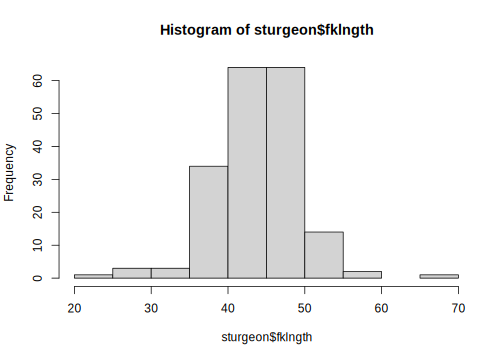
\includegraphics{Labo_BIO4558_files/figure-latex/hist-stur-1.pdf}

Les données semblent suivre approximativement une distribution normale.
C'est bon à savoir.
Cette syntaxe est un peu lourde puisqu'on doit ajouter le préfixe \texttt{sturgeon\$} devant chaque nom de variable.
On pourrait se faciliter la tâche en utilisant la commande \texttt{attach()} \textbf{mais cela est fortement déconseillé} et jamais utilisé dans ce document.

Cet histogramme est la représentation classique.
Mais les histogrammes ne sont pas parfaits.
Leur forme dépend en partie du nombre de catégories utilisées, surtout pour les petits échantillons.
On peut faire mieux, particulièrement si on est intéressé à comparer visuellement la distribution des observations à une distribution normale.
Mais il faut programmer un peu (ou savoir copier-coller\ldots{})

\begin{rmdcode}
Copiez-collez le code suivant dans une nouvelle fenêtre script ( File-\textgreater{}New script, ou Ctrl-n dans Windows), puis exécutez le.
\end{rmdcode}

\begin{Shaded}
\begin{Highlighting}[]
\KeywordTok{library}\NormalTok{(ggplot2)}
\CommentTok{#  use "sturgeon" dataframe to make plot called mygraph}
\CommentTok{#  and define x axis as representing fklngth}
\NormalTok{mygraph <-}\StringTok{ }\KeywordTok{ggplot}\NormalTok{(sturgeon, }\KeywordTok{aes}\NormalTok{(}\DataTypeTok{x =}\NormalTok{ fklngth))}
\CommentTok{#  add data to the mygraph ggplot}
\NormalTok{mygraph <-}\StringTok{ }\NormalTok{mygraph }\OperatorTok{+}
\CommentTok{#  add data density smooth}
\StringTok{    }\KeywordTok{geom_density}\NormalTok{() }\OperatorTok{+}
\CommentTok{#  add rug (bars at the bottom of the plot)}
\StringTok{    }\KeywordTok{geom_rug}\NormalTok{() }\OperatorTok{+}
\CommentTok{#  add black semitransparent histogram}
\StringTok{    }\KeywordTok{geom_histogram}\NormalTok{(}\KeywordTok{aes}\NormalTok{(}\DataTypeTok{y =}\NormalTok{ ..density..), }\DataTypeTok{bins =} \DecValTok{30}\NormalTok{, }\DataTypeTok{color =} \StringTok{"black"}\NormalTok{,   }\DataTypeTok{alpha =} \FloatTok{0.3}\NormalTok{) }\OperatorTok{+}
\CommentTok{#  add normal curve in red, with mean and sd from fklength}
\StringTok{    }\KeywordTok{stat_function}\NormalTok{(}\DataTypeTok{fun =}\NormalTok{ dnorm,}
                   \DataTypeTok{args =} \KeywordTok{list}\NormalTok{(}
                     \DataTypeTok{mean =} \KeywordTok{mean}\NormalTok{(sturgeon}\OperatorTok{$}\NormalTok{fklngth),}
                     \DataTypeTok{sd =} \KeywordTok{sd}\NormalTok{(sturgeon}\OperatorTok{$}\NormalTok{fklngth) ),}
                   \DataTypeTok{color =} \StringTok{"red"}\NormalTok{)}
\CommentTok{# display graph}
\NormalTok{    mygraph}
\end{Highlighting}
\end{Shaded}

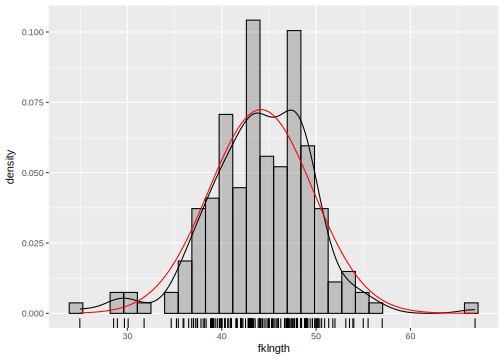
\includegraphics{Labo_BIO4558_files/figure-latex/stur-g1-1.pdf}

Chaque observation est représentée par une barre sous l'axe des x (rug).
En rouge est la distribution normale de données avec la même moyenne et écart-type que les observations.
Et l'autre ligne est la densité de probabilité empirique, « lissée » à partir des observations.
Si vous êtes plus aventureux, vous pouvez examiner la distribution des observations de fklngth par sous-groupes (par exemple sex et year) avec :

\begin{Shaded}
\begin{Highlighting}[]
\NormalTok{mygraph }\OperatorTok{+}\StringTok{ }\KeywordTok{facet_grid}\NormalTok{(year }\OperatorTok{~}\StringTok{ }\NormalTok{sex)}
\end{Highlighting}
\end{Shaded}

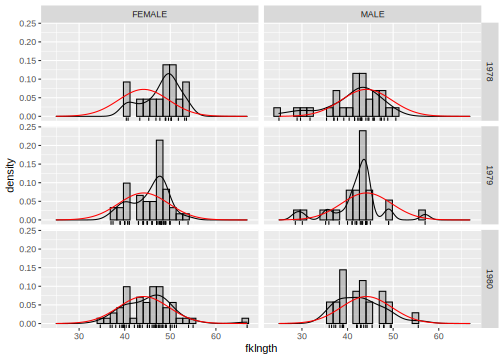
\includegraphics{Labo_BIO4558_files/figure-latex/aventure-1.pdf}

Chaque panneau illustre la distribution pour un sexe cette année-là, et la courbe en rouge récurrente représente la distribution normale pour l'ensemble des données.
Cette courbe peut servir à mieux évaluer visuellement les différences entre les panneaux.
Une autre façon d'évaluer la normalité de données visuellement est de faire un QQ plot avec la paire de commandes \texttt{qqnorm()} et \texttt{qqline()}.

\begin{Shaded}
\begin{Highlighting}[]
\KeywordTok{qqnorm}\NormalTok{(sturgeon}\OperatorTok{$}\NormalTok{fklngth)}
\KeywordTok{qqline}\NormalTok{(sturgeon}\OperatorTok{$}\NormalTok{fklngth)}
\end{Highlighting}
\end{Shaded}

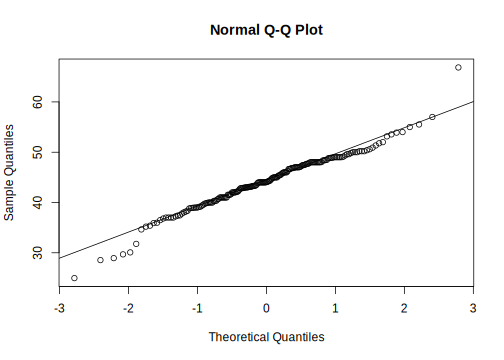
\includegraphics{Labo_BIO4558_files/figure-latex/stur-norm-1.pdf}

Des données parfaitement normales suivraient la ligne droite diagonale.
Ici, il y a des déviations dans les queues de la distribution, et un peu à droite du centre.
Comparez cette représentation à celle des deux graphiques précédents.
Vous conviendrez sans doute avec moi qu'il est plus facile de visualiser comment la distribution dévie de la normalité sur les histogrammes et les graphiques de la densité empirique de probabilité que sur les QQ plots.
Ceci dit, les QQ plots sont souvent utilisés et vous devriez être capable de les interpréter.
De plus, on peut facilement éprouver statistiquement l'hypothèse que les données sont distribuées normalement avec R par la commande \texttt{shapiro.test()} qui calcule une statistique (W) qui est une mesure de la tendance des points d'un QQ plot à former une ligne parfaite.
Si oui, alors W=1.
Si W s'éloigne de 1 (vers 0), alors les données s'éloignent de la normalité.
Ici,

\begin{Shaded}
\begin{Highlighting}[]
\KeywordTok{shapiro.test}\NormalTok{(sturgeon}\OperatorTok{$}\NormalTok{fklngth)}
\end{Highlighting}
\end{Shaded}

\begin{verbatim}
## 
## 	Shapiro-Wilk normality test
## 
## data:  sturgeon$fklngth
## W = 0.97225, p-value = 0.0009285
\end{verbatim}

W n'est pas très loin de 1, mais suffisamment pour que la différence soit significative.
L'examen visuel des grands échantillons est souvent compliqué par le fait que plusieurs points se superposent et qu'il devient plus difficile de bien visualiser la tendance centrale.
Les boxplots avec ``moustaches'' (box and whiskers plots) offrent une alternative intéressante.
La commande \texttt{boxplot()} peut produire un boxplot de fklngth pour chaque niveau de sex, et ajoute les coches.

\begin{Shaded}
\begin{Highlighting}[]
\KeywordTok{boxplot}\NormalTok{(fklngth }\OperatorTok{~}\StringTok{ }\NormalTok{sex, }\DataTypeTok{data =}\NormalTok{ sturgeon, }\DataTypeTok{notch =} \OtherTok{TRUE}\NormalTok{)}
\end{Highlighting}
\end{Shaded}

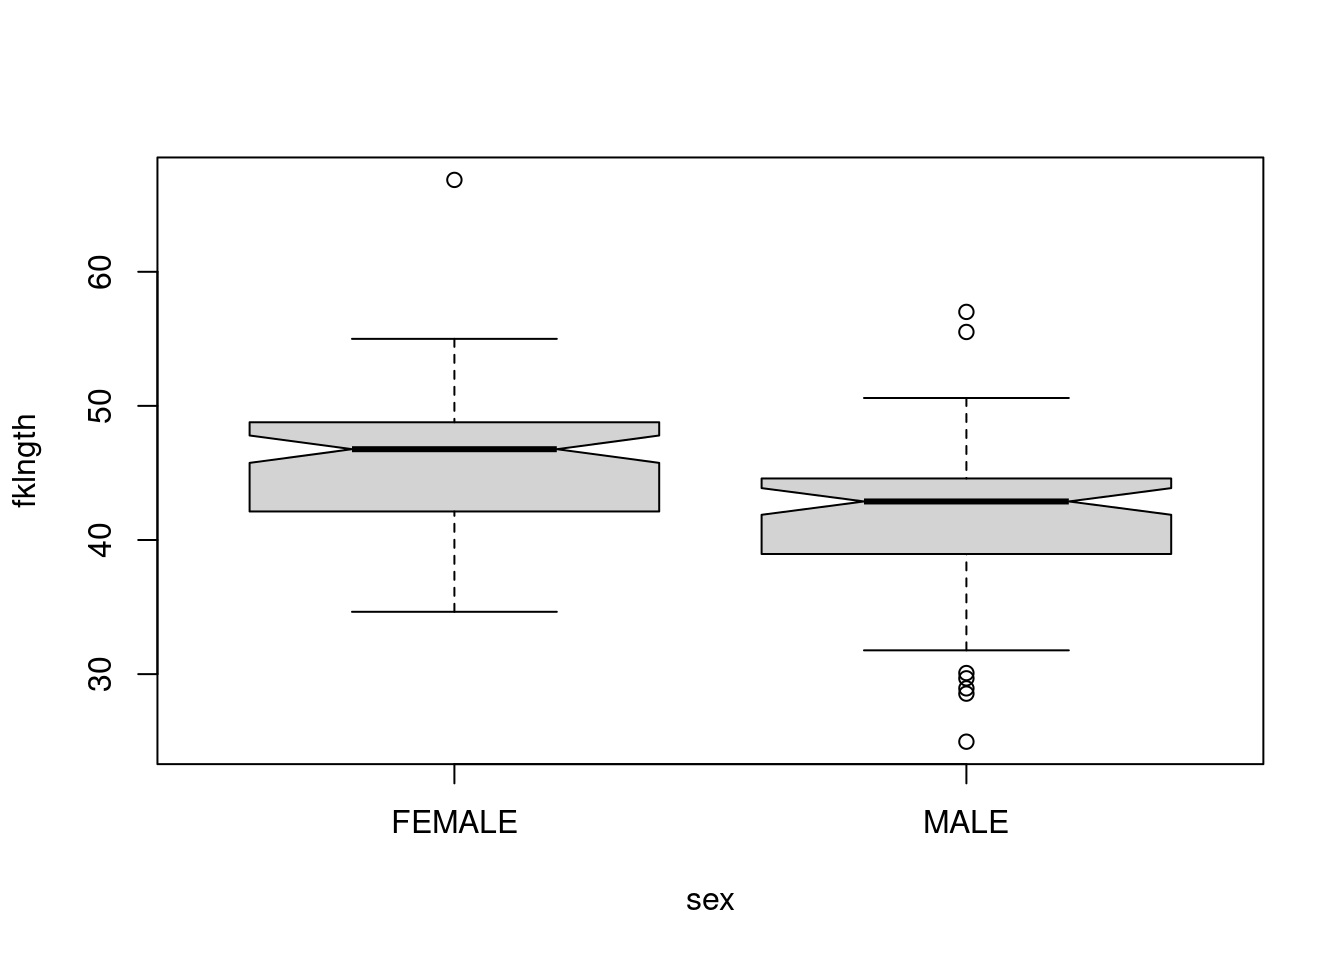
\includegraphics{Labo_BIO4558_files/figure-latex/boxplot-stur-1.pdf}

La ligne un peu plus épaisse dans la boîte de la Fig.7 indique la médiane.
La coche est proportionnelle à l'incertitude quant à la position de la médiane.
On peut visuellement interpréter approximativement les différences entre médianes en examinant si il y a chevauchement entre les coches (ici, il n'y a pas chevauchement, et on conclurait provisoirement que la médiane de fklngth pour les femelles est supérieure à celle des mâles).
Les boîtes s'étendent du premier au troisième quartile (du 25ième au 75ième percentile si vous préférez), Les barres (moustaches ou whiskers) au-dessus et en dessous des boîtes s'étendent soit de la valeur minimum à la valeur maximum, ou, si il y a des valeurs extrêmes, de la plus petite à la plus grande valeur à l'intérieur de 1.5x la largeur de l'étendue interquartile .
Enfin, les observations qui excèdent les limites des moustaches (donc à plus de 1.5x l'étendue interquartile de chaque côté de la médiane) sont indiquées par des symboles.Ce sont des valeurs qui pourraient être considérées comme extrêmes et possiblement aberrantes.

\hypertarget{diagrammes-de-dispersion-bivariuxe9s}{%
\subsection{Diagrammes de dispersion bivariés}\label{diagrammes-de-dispersion-bivariuxe9s}}

En plus des graphiques pour chacune des variables séparément, il est très souvent intéressant de jeter un coup d'oeil aux diagrammes de dispersion .
La commande \texttt{plot(y\textasciitilde{}x)} permet de faire le graphique de y sur l'axe vertical (l'ordonnée) en fonction de x sur l'axe horizontal (l'abscisse).

\begin{rmdcode}
Faites un graphique de fklngth en fonction de age avec la commande plot.
\end{rmdcode}

Vous devriez obtenir:

\begin{Shaded}
\begin{Highlighting}[]
\KeywordTok{plot}\NormalTok{(fklngth }\OperatorTok{~}\StringTok{ }\NormalTok{age, }\DataTypeTok{data =}\NormalTok{ sturgeon)}
\end{Highlighting}
\end{Shaded}

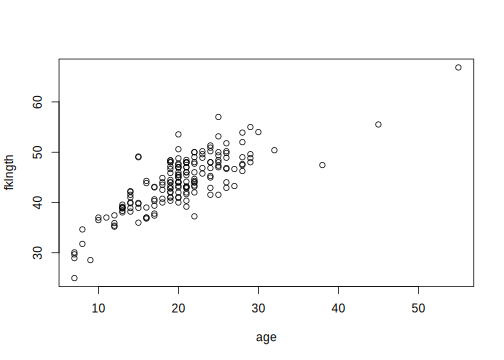
\includegraphics{Labo_BIO4558_files/figure-latex/stur-biv-plot-1.pdf}

R a une fonction qui permet la création des graphiques de dispersion de toutes les paires de variables (\texttt{pairs()}).
Une des option de ¬ est l'ajout d'une trace lowess qui indique la tendance de la relation entre les variables.
Pour obtenir la matrice de ces graphiques avec la trace lowess pour toutes les variable dans sturgeon, entrer la commande \texttt{pairs(sturgeon{[},1:6{]},\ panel=panel.smooth)} et vous devriez obtenir

\begin{Shaded}
\begin{Highlighting}[]
\KeywordTok{pairs}\NormalTok{(sturgeon[,}\DecValTok{1}\OperatorTok{:}\DecValTok{6}\NormalTok{], }\DataTypeTok{panel =}\NormalTok{ panel.smooth)}
\end{Highlighting}
\end{Shaded}

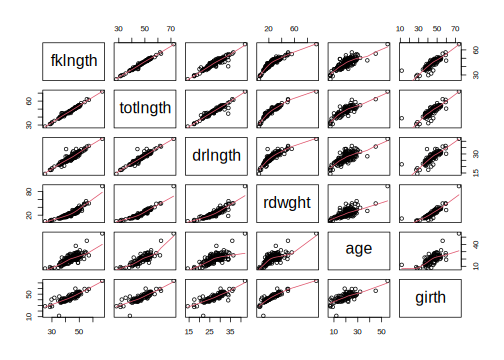
\includegraphics{Labo_BIO4558_files/figure-latex/pairs-stur-1.pdf}

\hypertarget{cruxe9er-des-sous-ensembles-de-cas}{%
\section{Créer des sous-ensembles de cas}\label{cruxe9er-des-sous-ensembles-de-cas}}

Il arrive fréquemment qu'une analyse se concentre sur un sous-ensemble des observations contenues dans un fichier de données.
Les cas sont d'habitude sélectionnés selon un critère en particulier.
Pour utiliser un sous-ensemble de vos données en créant un graphique ou en performant une analyse, on peut utiliser la commande \texttt{subset()}.
Par exemple, pour créer un sous ensemble des données du tableau sturgeon qui ne contient que les femelles capturées en 1978, on peut écrire :

\begin{Shaded}
\begin{Highlighting}[]
\NormalTok{sturgeon.female}\FloatTok{.1978}\NormalTok{ <-}\StringTok{ }\KeywordTok{subset}\NormalTok{(sturgeon, sex }\OperatorTok{==}\StringTok{ "FEMALE"} \OperatorTok{&}\StringTok{ }\NormalTok{year }\OperatorTok{==}\StringTok{ "1978"}\NormalTok{)}
\NormalTok{sturgeon.female}\FloatTok{.1978}
\end{Highlighting}
\end{Shaded}

\begin{verbatim}
##      fklngth totlngth  drlngth rdwght age girth    sex   location year
## 2   50.19685 54.13386 31.49606     NA  24  53.5 FEMALE    THE_PAS 1978
## 4   50.19685 53.14961 32.28346     NA  23  52.5 FEMALE    THE_PAS 1978
## 6   49.60630 53.93701 31.10236  35.86  23  54.2 FEMALE    THE_PAS 1978
## 7   47.71654 51.37795 33.97638  33.88  20  48.0 FEMALE    THE_PAS 1978
## 15  48.89764 53.93701 29.92126  35.86  23  52.5 FEMALE    THE_PAS 1978
## 105 46.85039       NA 28.34646  23.90  24    NA FEMALE CUMBERLAND 1978
## 106 40.74803       NA 24.80315  17.50  18    NA FEMALE CUMBERLAND 1978
## 107 40.35433       NA 25.59055  20.90  21    NA FEMALE CUMBERLAND 1978
## 109 43.30709       NA 27.95276  24.10  19    NA FEMALE CUMBERLAND 1978
## 113 53.54331       NA 33.85827  48.90  20    NA FEMALE CUMBERLAND 1978
## 114 51.77165       NA 31.49606  35.30  26    NA FEMALE CUMBERLAND 1978
## 116 45.27559       NA 26.57480  23.70  24    NA FEMALE CUMBERLAND 1978
## 118 53.14961       NA 32.67717  45.30  25    NA FEMALE CUMBERLAND 1978
## 119 50.19685       NA 32.08661  33.90  26    NA FEMALE CUMBERLAND 1978
## 123 49.01575       NA 29.13386  37.50  22    NA FEMALE CUMBERLAND 1978
\end{verbatim}

\begin{rmdcaution}
Dans ces comparaisons, il faut toujours utiliser \texttt{==} pour égal à.
Dans ce contexte, si vous utilisez \texttt{=} seulement, vous n'obtiendrez pas ce que vous désirez.
Dans le tableau qui suit se trouve une liste de commandes communes que vous allez probablement utiliser pour créer des expressions en R.
\end{rmdcaution}

\begin{longtable}[]{@{}llll@{}}
\toprule
Operateur & Explication & Operateur & Explication\tabularnewline
\midrule
\endhead
== & Égal à & != & Pas égal à\tabularnewline
\textgreater{} & Plus que & \textless{} & Moins que\tabularnewline
\textgreater{}= & Plus que ou égal à & \textless{}= & Moins que ou égal à\tabularnewline
\& & Et vectorisé & \textbar{} & Ou vectorisé\tabularnewline
\&\& & Et contrôle & \textbar{}\textbar{} & Ou contrôle\tabularnewline
! & Pas & &\tabularnewline
\bottomrule
\end{longtable}

\begin{itemize}
\tightlist
\item
  En utilisant les commandes \texttt{subset()} et \texttt{hist()}, essayez de faire un histogramme pour le sous-ensemble de cas correspondant aux femelles capturées en 1979 et 1980 (donc \texttt{sex\ ==\ "FEMALE"\ \&\ (year\ ==\ "1979"\ \textbar{}\ year\ ==\ "1980")})
\end{itemize}

\hypertarget{transformations-de-donnuxe9es}{%
\section{Transformations de données}\label{transformations-de-donnuxe9es}}

Il est très fréquemment nécessaire d'effectuer des transformations mathématiques sur les données brutes pour mieux satisfaire aux conditions d'application de tests statistiques.
R étant aussi un langage de programmation complet, il peut donc effectuer les transformations désirées.
Les fonctions les plus fréquemment utilisées sont:

\begin{itemize}
\tightlist
\item
  \texttt{log()}
\item
  \texttt{sqrt()}
\item
  \texttt{ifelse()}
\end{itemize}

On peut employer ces fonctions directement dans les lignes de commandes, ou encore créer de nouvelles variables orphelines ou faisant partie d'un data.frame.
Par exemple, pour faire un graphique du logarithme décimal de fklngth en fonction de l'âge, on peut écrire

\begin{Shaded}
\begin{Highlighting}[]
\KeywordTok{plot}\NormalTok{(}\KeywordTok{log}\NormalTok{(fklngth)}\OperatorTok{~}\NormalTok{age, }\DataTypeTok{data =}\NormalTok{ sturgeon)}
\end{Highlighting}
\end{Shaded}

Pour créer une variable orpheline (i.e.~non incluse dans le data.frame) appelée logfklngth et contenant le logarithme décimal de fklngth, on peut écrire

\begin{Shaded}
\begin{Highlighting}[]
\NormalTok{logfklngth <-}\StringTok{ }\KeywordTok{log10}\NormalTok{(sturgeon}\OperatorTok{$}\NormalTok{fklngth)}
\end{Highlighting}
\end{Shaded}

Si on veut ajouter cette variable transformée à un tableau de données (data.frame), alors, on doit préfixer le nom de la variable par le nom du base de données et du symbole \texttt{\$}, par exemple, pour ajouter une variable nommée \texttt{lfkl} contenant le log10 de fklngth au tableau sturgeon, on peut écrire:

\begin{Shaded}
\begin{Highlighting}[]
\NormalTok{sturgeon}\OperatorTok{$}\NormalTok{logfkl <-}\StringTok{ }\KeywordTok{log10}\NormalTok{(sturgeonfklngth)}
\end{Highlighting}
\end{Shaded}

N'oubliez pas de sauvegarder ce tableau modifié si vous voulez avoir accès à cette nouvelle variable dans le futur.
Pour les transformations conditionnelles, on peut utiliser la fonction \texttt{ifelse()}.
Par exemple, pour créer une nouvelle variable appelée dummy qui sera égale à 1 pour les mâles et 0 pour les femelles, on peut écrire:

\begin{Shaded}
\begin{Highlighting}[]
\NormalTok{sturgeon}\OperatorTok{$}\NormalTok{dummy <-}\StringTok{ }\KeywordTok{ifelse}\NormalTok{(sturgeon}\OperatorTok{$}\NormalTok{sex }\OperatorTok{==}\StringTok{ "MALE"}\NormalTok{, }\DecValTok{1}\NormalTok{, }\DecValTok{0}\NormalTok{)}
\end{Highlighting}
\end{Shaded}

\hypertarget{exercice-sur-r}{%
\section{Exercice sur R}\label{exercice-sur-r}}

\begin{rmdcode}
Vous trouverez dans le fichier salmonella, des valeurs numériques du ratio pour deux milieux (IN VITRO et IN VIVO) pour trois souches.
Examinez les données pour ratio et faites des graphiques pour évaluer la normalité de la distribution des ratios pour la souche SAUVAGE.
\end{rmdcode}

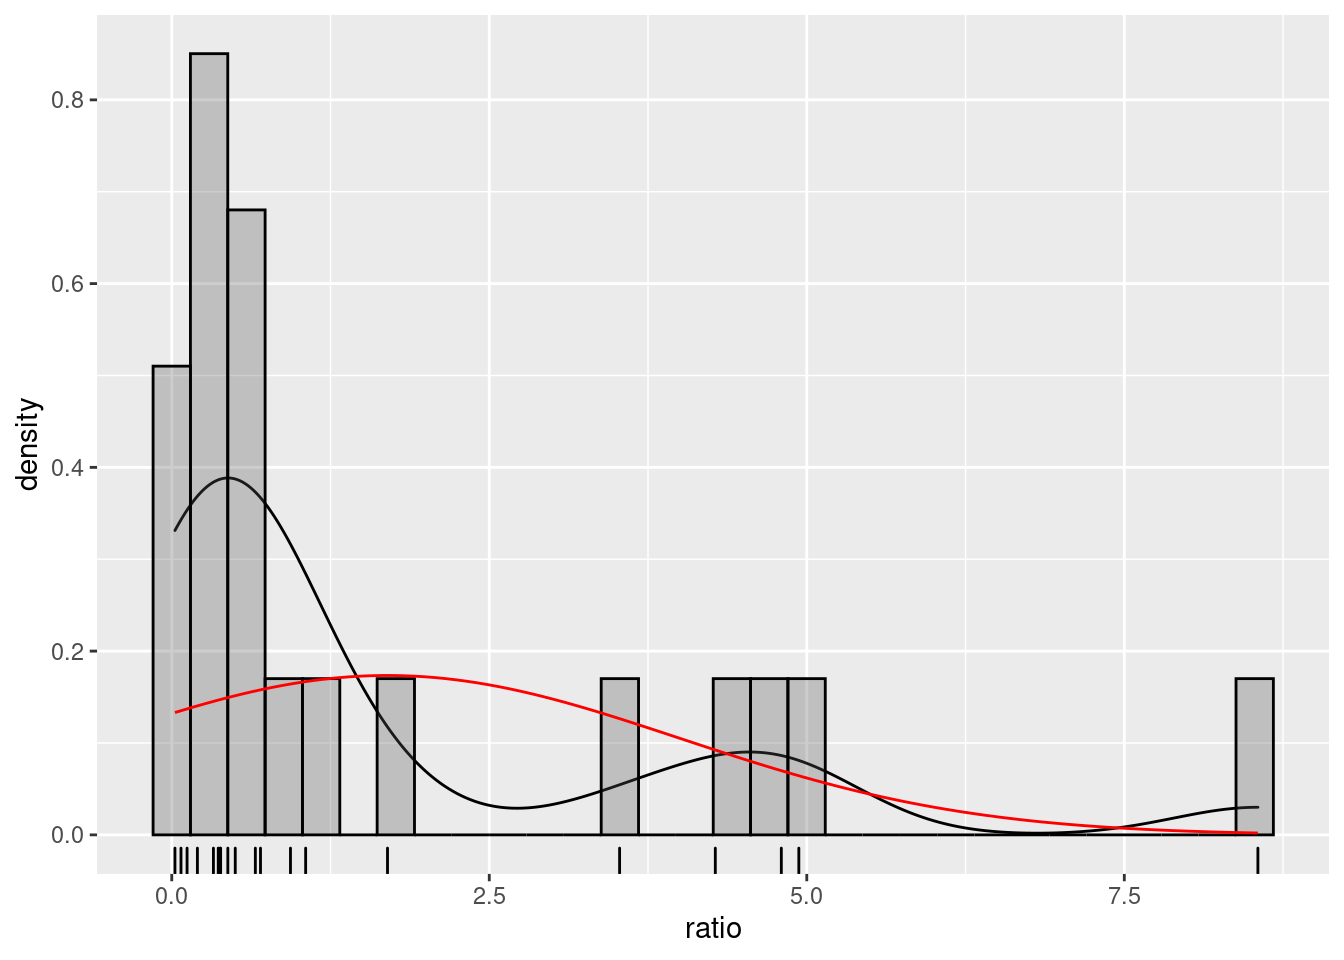
\includegraphics{Labo_BIO4558_files/figure-latex/intror-exer-1.pdf}

\hypertarget{analyse-de-puissance-avec-r-et-gpower}{%
\chapter{Analyse de puissance avec R et G*Power}\label{analyse-de-puissance-avec-r-et-gpower}}

Après avoir complété cet exercice de laboratoire, vous devriez :

\begin{itemize}
\tightlist
\item
  Pouvoir calculer la puissance d'un test de t avec R et G*Power
\item
  Pouvoir calculer l'effectif requis pour obtenir la puissance désirée avec un test de t
\item
  Pouvoir calculer la taille de l'effet détectable par un test de t étant donné l'effectif, la puissance et \(\alpha\)
\item
  Comprendre comment la puissance change lorsque l'effectif augmente, la taille de l'effet change, ou lorsque \(\alpha\) diminue
\item
  Comprendre comment la puissance est affectée lorsque l'on passe d'un test bilatéral à un test unilatéral
\end{itemize}

\hypertarget{la-thuxe9orie}{%
\section{La théorie}\label{la-thuxe9orie}}

\hypertarget{quest-ce-que-la-puissance}{%
\subsection{Qu'est-ce que la puissance?}\label{quest-ce-que-la-puissance}}

\emph{La puissance est la probabilité de rejeter l'hypothèse nulle quand elle est fausse.}

\hypertarget{pourquoi-faire-une-analyse-de-puissance}{%
\subsection{Pourquoi faire une analyse de puissance?}\label{pourquoi-faire-une-analyse-de-puissance}}

\hypertarget{uxe9valuer-luxe9vidence}{%
\subsubsection*{Évaluer l'évidence}\label{uxe9valuer-luxe9vidence}}


L'analyse de puissance effectuée après avoir accepté une hypothèse nulle permet de calculer la probabilité que l'hypothèse nulle soit rejetée si elle était fausse et que la taille de l'effet était d'une valeur donnée.
Ce type d'analyse a posteriori est très commun.

\hypertarget{planifier-de-meilleures-expuxe9riences}{%
\subsubsection*{Planifier de meilleures expériences}\label{planifier-de-meilleures-expuxe9riences}}


L'analyse de puissance effectuée avant de réaliser une expérience (le plus souvent après une expérience préliminaire cependant), permet de déterminer le nombre d'observations nécessaires pour détecter un effet d'une taille donnée à un niveau fixe de probabilité (la puissance).
Ce type d'analyse a priori devrait être réalisé plus souvent.

\hypertarget{estimer-la-limite-de-duxe9tection-statistique}{%
\subsubsection*{Estimer la ``limite de détection'' statistique}\label{estimer-la-limite-de-duxe9tection-statistique}}


L'effort d'échantillonnage est souvent déterminé à l'avance (par exemple lorsque vous héritez de données récoltées par quelqu'un d'autre), ou très sévèrement limité (lorsque les contraintes logistiques prévalent).
Que ce soit a priori ou a posteriori l'analyse de puissance vous permet d'estimer, pour un effort d'échantillonnage donné et un niveau de puissance fixe, quelle est la taille minimale de l'effet qui peut être détecté (comme étant statistiquement significatif).

\hypertarget{facteurs-qui-affectent-la-puissance}{%
\subsection{Facteurs qui affectent la puissance}\label{facteurs-qui-affectent-la-puissance}}

Il y a 3 facteurs qui affectent la puissance d'un test statistique.

\hypertarget{le-crituxe8re-de-duxe9cision}{%
\subsubsection*{Le critère de décision}\label{le-crituxe8re-de-duxe9cision}}


La puissance dépend de \(\alpha\), le seuil de probabilité auquel on rejette l'hypothèse nulle.
Si ce seuil est très strict (\emph{i.e.} si \(\alpha\) est fixé à une valeur très basse, comme 0.1\% ou p = 0.001), alors la puissance sera plus faible que si le seuil était moins strict.

\hypertarget{la-taille-de-luxe9chantillon}{%
\subsubsection*{La taille de l'échantillon}\label{la-taille-de-luxe9chantillon}}


Plus l'échantillon est grand, plus la puissance est élevée.
La capacité d'un test à détecter de petites différences comme étant statistiquement significatives augmente avec une augmentation du nombre d'observations.

\hypertarget{la-taille-de-leffet}{%
\subsubsection*{La taille de l'effet}\label{la-taille-de-leffet}}


Plus la taille de l'effet est grande, plus un test a de puissance.
Pour un échantillon de taille fixe, la capacité d'un test à détecter un effet comme étant statistiquement significatif est plus élevée si l'effet est grand que s'il est petit.
La taille de l'effet est en fait une mesure du degré de fausseté de l'hypothèse nulle.

\hypertarget{quest-ce-que-gpower}{%
\section{Qu'est ce que G*Power?}\label{quest-ce-que-gpower}}

G*Power est un programme gratuit, développé par des psychologues de l'Université de Dusseldorf en Allemagne.
Le programme existe en version Mac et Windows.
Il peut cependant être utilisé sous linux via Wine.
G*Power vous permettra d'effectuer une analyse de puissance pour la majorité des tests que nous verrons au cours de la session sans avoir à effectuer des calculs complexes ou farfouiller dans des tableaux ou des figures décrivant des distributions ou des courbes de puissance.
Il est possible de faire tous les analyses de G*power avec R, mais cela est nettement plus complexes, car il faut tous coder à la main. Dans les cas les plus simple le code R est aussi fourni.
G*power est vraiment un outil très utile que vous devrez maîtriser.

\begin{itemize}
\tightlist
\item
  Téléchargez le programme \textbf{\href{https://www.psychologie.hhu.de/arbeitsgruppen/allgemeine-psychologie-und-arbeitspsychologie/gpower.html}{ici}} et installez-le sur votre ordi et votre station de travail au laboratoire (si ce n'est déjà fait).*
\end{itemize}

\hypertarget{comment-utiliser-gpower}{%
\section{Comment utiliser G*Power}\label{comment-utiliser-gpower}}

\hypertarget{principe-guxe9nuxe9ral}{%
\subsection{Principe général}\label{principe-guxe9nuxe9ral}}

L'utilisation de G*Power implique généralement en trois étapes:

\begin{enumerate}
\def\labelenumi{\arabic{enumi}.}
\tightlist
\item
  Choisir le test approprié
\item
  Choisir l'un des 5 types d'analyses de puissance disponibles
\item
  Inscrire les valeurs des paramètres requis et cliquer sur Calculate
\end{enumerate}

\hypertarget{types-danalyses-de-puissance-disponibles}{%
\subsection{Types d'analyses de puissance disponibles}\label{types-danalyses-de-puissance-disponibles}}

\hypertarget{a-priori}{%
\subsubsection*{A priori}\label{a-priori}}


Calcule l'effectif requis pour une valeur de \(\alpha\), \(\beta\) et de taille d'effet donnée.
Ce type d'analyse est utile à l'étape de planification des expériences.

\hypertarget{compromis}{%
\subsubsection*{Compromis}\label{compromis}}


Calcule \(\alpha\) et \(\beta\) pour un rapport \(\beta / \alpha\) donné, un effectif fixe, et une taille d'effet donnée.
Ce type d'analyse est plus rarement utilisé (je ne l'ai jamais fait), mais peut être utile lorsque le rapport \(\beta / \alpha\) est d'intérêt, par exemple lorsque le coût d'une erreur de type I et de type II peut être quantifié.

\hypertarget{crituxe8re}{%
\subsubsection*{Critère}\label{crituxe8re}}


Calcule \(\alpha\) pour \(\beta\), effectif et taille d'effet donné.
En pratique, je vois peu d'utilité pour ce type de calcul.
Contactez-moi si vous en voyez une!

\hypertarget{post-hoc}{%
\subsubsection*{Post-hoc}\label{post-hoc}}


Calcule la puissance (1 - \(\beta\)) pour \(\alpha\), une taille d'effet et un effectif donné.
Très utilisée pour interpréter les résultats d'une analyse statistique non-significative, mais seulement si l'on utilise une taille d'effet biologiquement significative (et non la taille d'effet observée).
Peu pertinente lorsque le test est significatif.

\hypertarget{sensitivituxe9}{%
\subsubsection*{Sensitivité}\label{sensitivituxe9}}


Calcule la taille d'effet détectable pour une valeur d'\(\alpha\), \(\beta\) et un effectif donné.
Très utile également au stade de planification des expériences.

\hypertarget{comment-calculer-la-taille-de-leffet-gpower-permet-de-faire-une-analyse-de-puissance-pour-de-nombreux-tests-statistiques}{%
\subsection{Comment calculer la taille de l'effet G*Power permet de faire une analyse de puissance pour de nombreux tests statistiques}\label{comment-calculer-la-taille-de-leffet-gpower-permet-de-faire-une-analyse-de-puissance-pour-de-nombreux-tests-statistiques}}

L'indice de la taille de l'effet qui est utilisé par G*Power pour les calculs dépend du test.
Notez que d'autres logiciels peuvent utiliser des indices différents et il est important de vérifier que l'indice que l'on utilise est celui qui convient.
G*Power vous facilite la tâche et permet de calculer la taille de l'effet en inscrivant seulement les valeurs pertinentes dans la fenêtre de calcul.
Le tableau suivant donne les indices utilisés par G*Power pour les différents tests.

\begin{longtable}[]{@{}lcl@{}}
\toprule
\begin{minipage}[b]{0.11\columnwidth}\raggedright
Test\strut
\end{minipage} & \begin{minipage}[b]{0.35\columnwidth}\centering
Taille d'effet\strut
\end{minipage} & \begin{minipage}[b]{0.46\columnwidth}\raggedright
Formule\strut
\end{minipage}\tabularnewline
\midrule
\endhead
\begin{minipage}[t]{0.11\columnwidth}\raggedright
test de t sur des moyennes\strut
\end{minipage} & \begin{minipage}[t]{0.35\columnwidth}\centering
d\strut
\end{minipage} & \begin{minipage}[t]{0.46\columnwidth}\raggedright
\(d = \frac{|\mu_1 - \mu_2|}{\sqrt{({s_1}^2 + {s_2}^2)/2}}\)\strut
\end{minipage}\tabularnewline
\begin{minipage}[t]{0.11\columnwidth}\raggedright
test de t pour des corrélations\strut
\end{minipage} & \begin{minipage}[t]{0.35\columnwidth}\centering
r\strut
\end{minipage} & \begin{minipage}[t]{0.46\columnwidth}\raggedright
\strut
\end{minipage}\tabularnewline
\begin{minipage}[t]{0.11\columnwidth}\raggedright
autres tests de t\strut
\end{minipage} & \begin{minipage}[t]{0.35\columnwidth}\centering
f\strut
\end{minipage} & \begin{minipage}[t]{0.46\columnwidth}\raggedright
\(f = \frac{\mu_1}{\sigma}\)\strut
\end{minipage}\tabularnewline
\begin{minipage}[t]{0.11\columnwidth}\raggedright
test F (ANOVA)\strut
\end{minipage} & \begin{minipage}[t]{0.35\columnwidth}\centering
f\strut
\end{minipage} & \begin{minipage}[t]{0.46\columnwidth}\raggedright
\(f = \frac{\frac{\sqrt{\sum_{i=1}^k (\mu_i - \mu)^2}}{k}}{\sigma}\)\strut
\end{minipage}\tabularnewline
\begin{minipage}[t]{0.11\columnwidth}\raggedright
autres test F\strut
\end{minipage} & \begin{minipage}[t]{0.35\columnwidth}\centering
\(f^2\)\strut
\end{minipage} & \begin{minipage}[t]{0.46\columnwidth}\raggedright
\(f^2 = \frac{{R_p}^2}{1-{R_p}^2}\)\strut
\end{minipage}\tabularnewline
\begin{minipage}[t]{0.11\columnwidth}\raggedright
\strut
\end{minipage} & \begin{minipage}[t]{0.35\columnwidth}\centering
\strut
\end{minipage} & \begin{minipage}[t]{0.46\columnwidth}\raggedright
\({R_p}\) est le coefficient de corrélation partiel\strut
\end{minipage}\tabularnewline
\begin{minipage}[t]{0.11\columnwidth}\raggedright
test Chi-carré\strut
\end{minipage} & \begin{minipage}[t]{0.35\columnwidth}\centering
w\strut
\end{minipage} & \begin{minipage}[t]{0.46\columnwidth}\raggedright
\(w = \sqrt{ \sum_{i=1}^m \frac{(p_{0i} - p_{1i})^2 }{ p_{0i}} }\)\strut
\end{minipage}\tabularnewline
\begin{minipage}[t]{0.11\columnwidth}\raggedright
\strut
\end{minipage} & \begin{minipage}[t]{0.35\columnwidth}\centering
\strut
\end{minipage} & \begin{minipage}[t]{0.46\columnwidth}\raggedright
\(p_{0i}\) \(p_{1i}\) sont les proportions de la catégorie i prédites par l'hypothèse nulle et alternative respectivement\strut
\end{minipage}\tabularnewline
\bottomrule
\end{longtable}

\hypertarget{puissance-pour-un-test-de-t-comparant-deux-moyennes}{%
\section{Puissance pour un test de t comparant deux moyennes}\label{puissance-pour-un-test-de-t-comparant-deux-moyennes}}

L'objectif de cette séance de laboratoire est de vous familiariser avec G*Power et de vous aider à comprendre comment les quatre paramètres des analyses de puissance (\(\alpha\), \(\beta\), effectif et taille de l'effet) sont reliés entre eux.
On examinera seulement un des nombreux tests, le test de t permettant de comparer deux moyennes indépendantes.
C'est le test le plus communément utilisé par les biologistes, vous l'avez tous déjà utilisé, et il conviendra très bien pour les besoins de la cause.
Ce que vous apprendrez aujourd'hui s'appliquera à toutes les autres analyses de puissance que vous effectuerez à l'avenir.

Jaynie Stephenson a étudié la productivité des ruisseaux de la région d'Ottawa.
Elle a, entre autres, quantifié la biomasse des poissons dans 18 ruisseaux sur le Bouclier Canadien d'une part, et dans 18 autres ruisseaux de la vallée de la rivière des Outaouais et de la rivière Rideau d'autre part.
Elle a observé une biomasse plus faible dans les ruisseaux de la vallée (2.64 \(g/m^2\) , écart-type=3.28) que dans ceux du Bouclier (3.31 \(g/m^2\) , écart-type=2.79).
En faisant un test de t pour éprouver l'hypothèse nulle que la biomasse des poissons est la même dans les deux régions, elle obtient:

\begin{verbatim}
Pooled-Variance Two-Sample t-Test
t = -0.5746, df = 34, p-value = 0.5693
\end{verbatim}

Elle accepte l'hypothèse nulle (puisque p est plus élevé que 0.05) conclue donc que la biomasse moyenne des poissons est la même dans ces deux régions.

\hypertarget{analyse-post-hoc}{%
\subsection{Analyse post-hoc}\label{analyse-post-hoc}}

Compte tenu des valeurs des moyennes observées et de leur écart- type, on peut utiliser G*Power pour calculer la puissance du test de t bilatéral pour deux moyennes indépendantes et pour la taille d'effet (i.e.~la différence entre la biomasse entre les deux régions, pondérée par les écarts-type) à \(\alpha\) = 0.05.

Démarrer G*Power.

\begin{enumerate}
\def\labelenumi{\arabic{enumi}.}
\tightlist
\item
  À \textbf{Test family}, choisir: t tests
\item
  À \textbf{Statistical test}, choisir: Means: Difference between two inde- pendent means (two groups)
\item
  À \textbf{Type of power analysis}, choisir: Post hoc: Compute achieved power - given \(\alpha\), sample size, and effect size
\item
  Dans \textbf{Input Parameters},
\end{enumerate}

\begin{itemize}
\tightlist
\item
  à la boîte \textbf{Tail(s)}, choisir: Two,
\item
  vérifier que \(\alpha\) \textbf{err prob} est égal à 0.05
\item
  inscrire 18 pour \textbf{Sample size group} 1 et 2
\item
  pour calculer la taille d'effet (Effect size d), cliquer sur le bouton \textbf{Determine =\textgreater{}}
\end{itemize}

\begin{enumerate}
\def\labelenumi{\arabic{enumi}.}
\setcounter{enumi}{4}
\tightlist
\item
  Dans la fenêtre qui s'ouvre à droite, sélectionner \textbf{n1 = n2}
\end{enumerate}

\begin{itemize}
\tightlist
\item
  entrer les moyennes (\textbf{Mean group} 1 et 2)
\item
  entrer les écarts types (\textbf{SDs group} 1 et 2)
\item
  cliquer sur le bouton \textbf{Calculate and transfer to main window}
\end{itemize}

\begin{enumerate}
\def\labelenumi{\arabic{enumi}.}
\setcounter{enumi}{5}
\tightlist
\item
  Cliquer sur le bouton Calculate dans la fenêtre principale et vous devriez obtenir ceci:
\end{enumerate}

\begin{figure}
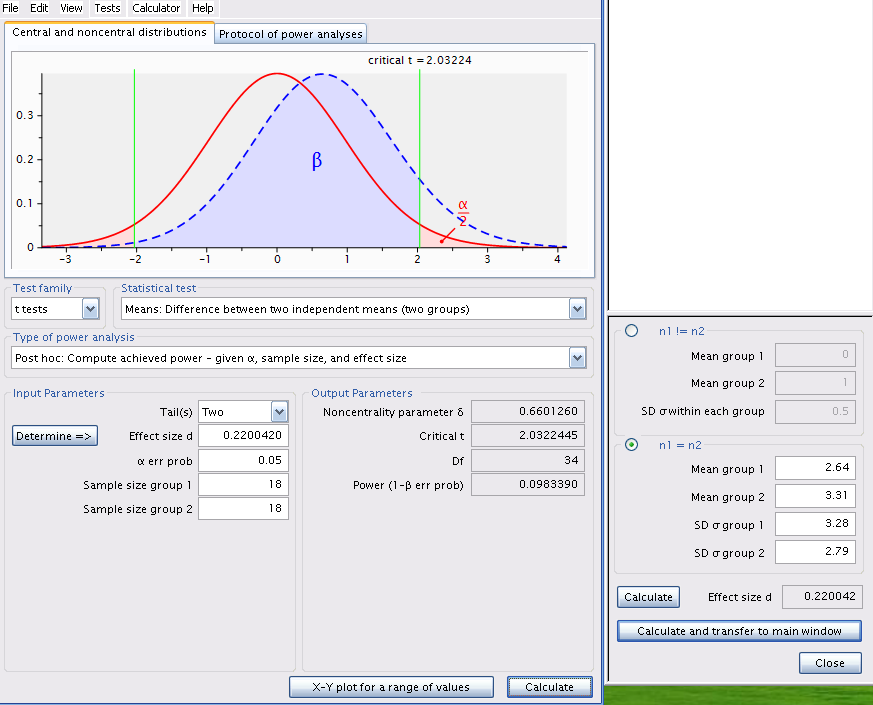
\includegraphics[width=1\linewidth]{images/gpower_1} \caption{Analyse post-hoc avec la taille d'effet estimée}\label{fig:gpower-1}
\end{figure}

Étudions un peu ce graphique.

\begin{itemize}
\tightlist
\item
  La courbe de gauche, en rouge, correspond à la distribution de la statistique t si \(H_0\) est vraie (i.e si les deux moyennes étaient égales) compte tenu de l'effectif (18 dans chaque région) et des écarts- types observés.
\item
  Les lignes verticales vertes correspondent aux valeurs critiques de t pour une valeur \(\alpha = 0.05\) et un effectif total de 36 (2x18).
\item
  Les régions ombrées en rose correspondent aux zones de rejet de \(H_0\).
  Si Jaynie avait obtenu une valeur de t en dehors de l'intervalle délimité par les valeurs critiques allant de -2.03224 à 2.03224, alors elle aurait rejeté \(H_0\) , l'hypothèse nulle d'égalité des deux moyennes.
  En fait, elle a obtenu une valeur de t égale à -0.5746 et conclu que la biomasse est la même dans les deux régions.
\item
  La courbe de droite, en bleu, correspond à la distribution de la sta- tistique t si \(H_1\) est vraie (ici \(H_1\) correspond à une différence de biomasse entre les deux régions de \(3.33-2.64=0.69g/m^2\) , compte tenu des écarts-types observés).
  Cette distribution correspond à ce qu'on devrait s'attendre à observer si \(H_1\) était vraie et que l'on répétait un grand nombre de fois les mesures dans des échantillons aléatoires de 18 ruisseaux des deux régions en calculant la statistique t à chaque fois.
  En moyenne, on observerait une valeur de t d'environ 0.6.
\item
  Notez que la distribution de droite chevauche considérablement celle de gauche, et une bonne partie de la surface sous la courbe de droite se retrouve à l'intérieur de l'intervalle d'acceptation de \(H_0\), délimité par les deux lignes vertes et allant de -2.03224 à 2.03224.
  Cette proportion, correspondant à la partie ombrée en bleu sous la courbe de droite et dénoté par \(\beta\) correspond au risque d'erreur de type II qui est d'accepter \(H_0\) quand \(H_1\) est vraie.
\item
  La puissance est simplement \(1-\beta\), et est ici de 0.098339.
  Donc, si la biomasse différait de 0.69\(g/m^2\) entre les deux régions, Jaynie n'avait que 9.8\% des chances d'être capable de détecter une différence statistiquement significative à \(\alpha=5%
  \) en échantillonnant 18 ruisseaux de chaque région.
\end{itemize}

\textbf{Récapitulons:} La différence de biomasse entre les deux régions n'est pas statistiquement significative d'après le test de t.
C'est donc que cette différence est relativement petite compte tenu de la précision des mesures.
Il n'est donc pas très surprenant que la puissance, i.e.~la probabilité de détecter une différence significative, soit faible.
Toute cette analyse ne nous informe pas beaucoup.

\textbf{Une analyse de puissance post hoc avec la taille de l'effet observé n'est pas très utile.}
On la fera plutôt pour une taille d'effet autre que celle observée quand H 0 est acceptée.
Quelle taille d'effet utiliser? C'est la biologie du système étudié qui peut nous guider.
Par exemple, en ce qui concerne la biomasse des poissons, on pourrait s'attendre à ce qu'une différence de biomasse du simple au double (disons de 2.64 à 5.28 \(g/m^2\) ) ait des conséquences écologiques.
On voudrait s'assurer que Jaynie avait de bonnes chances de détecter une différence aussi grande que celle-là avant d'accepter ses conclusions que la biomasse est la même entre les deux régions.
Quelles étaient les chances de Jaynie de détecter une différence de 2.64 \(g/m^2\) entre les deux régions? G*Power peut nous le dire.

\begin{itemize}
\tightlist
\item
  Changer la moyenne du groupe 2 à 5.28, recalculer la taille d'effet, et cliquer sur Calculate pour obtenir (\ref{fig:gpower-2}):
\end{itemize}

\begin{figure}
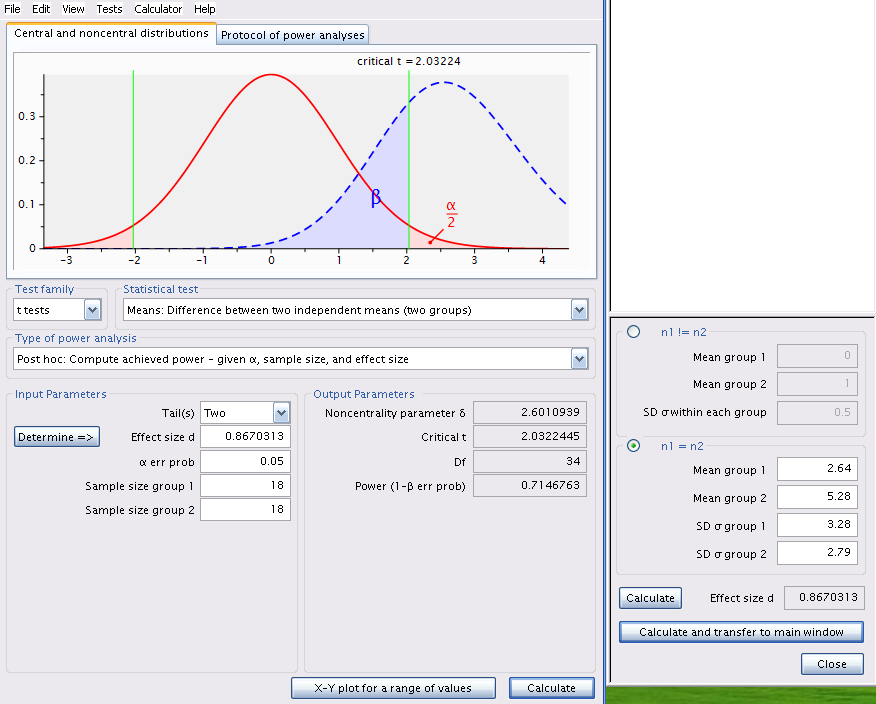
\includegraphics[width=1\linewidth]{images/gpower_2} \caption{Analyse post-hoc avec une taille d'effet différente}\label{fig:gpower-2}
\end{figure}

La puissance est de 0.71, donc Jaynie avait une chance raisonnable de détecter une différence du simple au double avec 18 ruisseaux dans chaque région.

Notez que cette analyse de puissance post hoc pour une taille d'effet jugée biologiquement significative est bien plus informative que l'analyse précédente pour la taille d'effet observée (qui est celle effectuée par défaut par bien des néophytes et de trop nombreux logiciels qui essaient de penser pour nous).
En effet, Jaynie n'a pu détecter de différences significatives entre les deux régions.
Cela pourrait être pour deux raisons: soit qu'il n'y a pas de différences entre les régions, ou soit parce que la précision des mesures est si faible et l'effort d'échantillonnage était si limité qu'il était très peu probable de détecter même d'énormes différences.
La deuxième analyse de puissance permet d'éliminer cette seconde possibilité puisque Jaynie avait 71\% des chances de détecter une différence du simple au double.

\hypertarget{analyse-uxe0-priori}{%
\subsection{Analyse à priori}\label{analyse-uxe0-priori}}

Supposons qu'on puisse défendre la position qu'une différence de biomasse observée par Jaynie entre les deux régions, \(3.31- 2.64=0.67g/m^2\) , soit écologiquement signifiante.
On devrait donc planifier la prochaine saison d'échantillonnage de manière à avoir de bonnes chances de détecter une différence de cette taille.
Combien de ruisseaux Jaynie devrait-elle échantillonner pour avoir 80\% des chances de la détecter (compte tenu de la variabilité observée)?

\begin{itemize}
\tightlist
\item
  Changer le type d'analyse de puissance dans G*Power à \textbf{A priori}: \textbf{Compute sample size - given \(\alpha\) , power, and effect size.}
  Assurez-vous que les valeurs pour les moyennes et les écarts-type soient celles qu'a obtenu Jaynie, recalculez la taille de l'effet, et inscrivez 0.8 pour la puissance et vous obtiendrez:
\end{itemize}

\begin{figure}
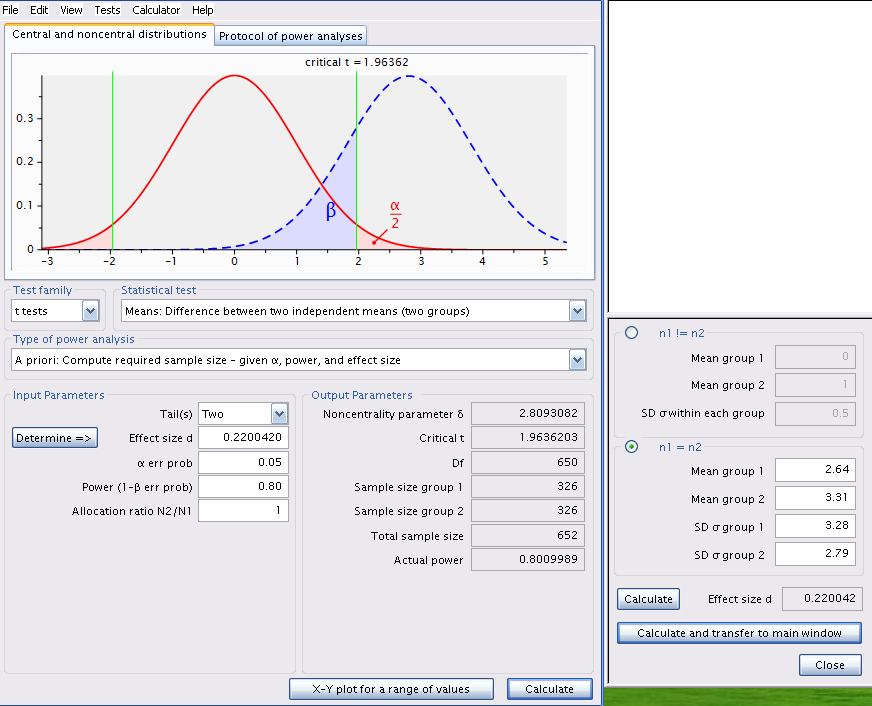
\includegraphics[width=1\linewidth]{images/gpower_3} \caption{Analyse à priori}\label{fig:gpower-3}
\end{figure}

\textbf{Ouch!} Il faudrait échantillonner 326 ruisseaux dans chaque région! Cela coûterait une fortune et exigerait de nombreuses équipes de travail.
Sans cela, on ne pourrait échantillonner que quelques dizaines de ruisseaux, et il serait peu probable que l'on puisse détecter une si faible différence de biomasse entre les deux régions.
Ce serait vraisemblablement en vain et pourrait être considéré comme une perte de temps: pourquoi tant d'efforts et de dépenses si les chances de succès sont si faibles.

Si on refait le même calcul pour une puissance de 95\%, on obtient 538 ruisseaux par région.
Augmenter la puissance ça demande plus d'effort.

\hypertarget{analyse-de-sensitivituxe9---calculer-la-taille-deffet-duxe9tectable}{%
\subsection{Analyse de sensitivité - Calculer la taille d'effet détectable}\label{analyse-de-sensitivituxe9---calculer-la-taille-deffet-duxe9tectable}}

Compte tenu de la variabilité observée, d'un effort d'échantillonnage de 18 ruisseaux par région, et en conservant \(\alpha=0.05\), quelle est la taille d'effet que Jaynie pouvait détecter avec 80\% de chances \(\beta=0.2\))?

\begin{itemize}
\tightlist
\item
  Changez le type d'analyse dans G*Power à \textbf{Sensitivity}: \textbf{Compute required effect size - given \(\alpha\) , power, and sample size} et assurez-vous que la taille des échantillons est de 18 dans chaque région.
  Vous obtiendrez:
\end{itemize}

\begin{figure}

\includegraphics[width=1\linewidth]{images/gpower_4} \caption{Analyse de sensitivité}\label{fig:gpower-4}
\end{figure}

La taille d'effet détectable pour cette taille d'échantillon, \(\alpha=0.05\) et \(\beta=0.2\) (ou une puissance de 80\%) est de 0.961296.
\textbf{Attention}, cette valeur est l'indice \texttt{d} de la taille de l'effet et est pondérée par la variabilité des mesures.
Dans ce cas ci, \texttt{d} est approximativement égal à
\[ d = \frac{| \bar{X_1} \bar{X_2} |} {\sqrt{\frac{{s_1}^2 +{s_2}^2}{2}}}\]
Pour convertir cette valeur de d sans unités en une valeur de différence de biomasse détectable (i.e \(| \bar{X_1} \bar{X_2} |\)), il suffit de multiplier d par le dénominateur de l'équation.
\[
| \bar{X_1} \bar{X_2} | = d * \sqrt{\frac{{s_1}^2 +{s_2}^2}{2}}
\]
Donc, avec 18 ruisseaux dans chaque région, pour \(\alpha=0.05\) et \(\beta=0.2\) (une puissance de 80\%), Jaynie pouvait détecter une différence de biomasse de 2.93\(g/m^2\) entre les régions, un peu plus que du simple au double.

\hypertarget{points-uxe0-retenir}{%
\section{Points à retenir}\label{points-uxe0-retenir}}

\begin{itemize}
\tightlist
\item
  L'analyse de puissance post hoc n'est pertinente que lorsque l'on a accepté l'hypothèse nulle.
  Il est en effet impossible de faire une erreur de type II quand on rejette \(H_0\).
\item
  Avec de très grands échantillons, on a une puissance quasi infinie et on peut détecter statistiquement de très petites différences qui ne sont pas nécessairement biologiquement significatives.
\item
  En utilisant un critère de signification plus strict (\(\alpha\)\textless{}0.05) on diminue notre puissance.
\item
  En voulant maximiser la puissance, on augmente l'effort requis, à moins d'utiliser une valeur critique plus libérale (\(\alpha>0.05\))
\item
  Le choix de \(\beta\) est quelque peu arbitraire.
  On considère que \(\beta=0.2\) (puissance de 80\%) est relativement élevé.
\end{itemize}

\hypertarget{exercice-sur-la-puissance}{%
\section{Exercice sur la puissance}\label{exercice-sur-la-puissance}}

\begin{rmdcode}
Les larves de mouches noires (Diptera: Simuliidae) ont été échantillonnées en février à l'émissaire de deux lacs des Cantons de l'Est (lacs Orford et Lovering).
La longueur de chaque larve a été mesurée.
Les données sont dans le fichier simulies.RData La relation entre la longueur (L, en mm) et la masse (M, en \(\mu\)g) pour l'espèce dominante (\emph{P. mixtum/fuscum}) est:

\[
M = 1.36 L^3.05
\]

\begin{enumerate}
\def\labelenumi{\arabic{enumi}.}
\tightlist
\item
  Calculer la masse moyenne et l'écart-type à chaque site.
\item
  En utilisant la masse moyenne de \emph{P. mixtum/fuscum} à Lovering comme référence et les écarts-types observés aux 2 sites, calculer la puissance d'un test de t bilatéral pour moyennes indépendantes

  \begin{enumerate}
  \def\labelenumii{\alph{enumii})}
  \tightlist
  \item
    si la différence de masse est de 5 \(\mu\)g, \(\alpha\) = 0.05, et qu'on échantillonnait 100 larves à chaque site
  \item
    si la différence de masse est de 20 \(\mu\)g, \(\alpha\) = 0.05, et qu'on échantillonnait 100 larves à chaque site
  \item
    si la différence de masse est de 50\(\mu\)g, \(\alpha\) = 0.05, et qu'on échantillonnait 100 larves à chaque site
  \item
    Comment est-ce que la puissance varie avec la taille de l'effet?
  \end{enumerate}
\item
  Calculer la taille d'échantillon requis pour pouvoir détecter, par un test de t bilatéral pour moyennes indépendantes en tenant compte des écarts-types observés, une différence de 50 \(\mu\)g entre les moyennes

  \begin{enumerate}
  \def\labelenumii{\alph{enumii})}
  \tightlist
  \item
    avec une puissance de 80\% et \(\alpha\) = 0.05
  \item
    avec une puissance de 80\% et \(\alpha\) = 0.001
  \item
    avec une puissance de 95\% et \(\alpha\) = 0.05
  \item
    Comment est-ce que la taille d'échantillon requise varie avec \(\alpha\) et \(\beta\)?
  \end{enumerate}
\item
  Calculer la taille d'effet détectable (d) par un test de t bilatéral pour moyennes indépendantes, compte tenu des écarts-types observés

  \begin{enumerate}
  \def\labelenumii{\alph{enumii})}
  \tightlist
  \item
    avec une puissance de 80\%, \(\alpha\) = 0.05, et des mesures sur 10 larves de chaque site
  \item
    avec une puissance de 80\%, \(\alpha\) = 0.05, et des mesures sur 200 larves à chaque site
  \item
    avec une puissance de 80\%, \(\alpha\) =0.05, et des mesures sur 20 larves d'un site et sur 380 larves au second site
  \item
    Comment est-ce que la taille d'effet détectable dépend de la taille d'échantillon dans les 2 groupes?
  \end{enumerate}
\item
  Calculer la différence de masse, en \(\mu\)g, qui est détectable d'après vos estimés de la taille minimale d'effet détectable à 4a, b, et c.
\end{enumerate}
\end{rmdcode}

\hypertarget{corruxe9lation-et-ruxe9gression-linuxe9aire-simple}{%
\chapter{Corrélation et régression linéaire simple}\label{corruxe9lation-et-ruxe9gression-linuxe9aire-simple}}

Après avoir complété cet exercice de laboratoire, vous devriez être en mesure de :

\begin{itemize}
\tightlist
\item
  Utiliser R pour produire un diagramme de dispersion pour illus-
  trer la relation entre deux variables avec trace lowess
\item
  Utiliser R pour faire des transformations simples
\item
  Utiliser R pour calculer le coefficient de corrélation de Pearson entre deux variables et en évaluer sa signification statistique
\item
  Utiliser R pour calculer la corrélation de rang entre des paires de variables avec le r de Spearman et le tau de Kendall
\item
  Utiliser R pour évaluer la signification de corrélations dans une matrice de corrélation en utilisant les probabilités ajustées par la méthode de Bonferroni.
\item
  Utiliser R pour faire une régression linéaire simple.
\item
  Utiliser R pour évaluer si un ensemble de données remplit les conditions d'application d'une analyse de régression simple.
\item
  Quantifier la taille de l'effet d'une régression simple et effectuer une analyse de puissance avec G*Power.
\end{itemize}

\hypertarget{set-lm}{%
\section{Paquets et données requises pour le labo}\label{set-lm}}

Ce laboratoire nécessite:

\begin{itemize}
\tightlist
\item
  les paquets R:

  \begin{itemize}
  \tightlist
  \item
    car
  \item
    lmtest
  \item
    boot
  \end{itemize}
\item
  les fichiers de données

  \begin{itemize}
  \tightlist
  \item
    sturgeon.csv
  \end{itemize}
\end{itemize}

\hypertarget{diagrammes-de-dispersion}{%
\section{Diagrammes de dispersion}\label{diagrammes-de-dispersion}}

Les analyses de corrélation et de régression devraient toujours commencer par un examen des données.C'est une étape critique qui sert à évaluer si ce type d'analyse est approprié pour un ensemble de données.
Supposons que nous sommes intéressés à évaluer si la longueur d'esturgeons mâles dans la région de \emph{The Pas} covarie avec leur poids.
Pour répondre à cette question, regardons d'abord la corrélation entre
la longueur et le poids.
Souvenez-vous qu'une des conditions d'application de l'analyse de
corrélation est que la relation entre les deux variables est linéaire. Pour
évaluer cela, commençons par faire un diagramme de dispersion.

\begin{itemize}
\tightlist
\item
  Les données sur les esturgeons son disponibles dans le fichier \texttt{sturgeon.csv}.
  Après avoir chargé les données dnas un objet \texttt{sturgeon}, faites un diagramme de dispersion avec une droite de régression et une courbe LOWESS de la longueur en fonction du poids.
\end{itemize}

\begin{Shaded}
\begin{Highlighting}[]
\NormalTok{sturgeon <-}\StringTok{ }\KeywordTok{read.csv}\NormalTok{(}\StringTok{"data/sturgeon.csv"}\NormalTok{)}
\KeywordTok{str}\NormalTok{(sturgeon)}
\end{Highlighting}
\end{Shaded}

\begin{verbatim}
## 'data.frame':	186 obs. of  9 variables:
##  $ fklngth : num  37 50.2 28.9 50.2 45.6 ...
##  $ totlngth: num  40.7 54.1 31.3 53.1 49.5 ...
##  $ drlngth : num  23.6 31.5 17.3 32.3 32.1 ...
##  $ rdwght  : num  15.95 NA 6.49 NA 29.92 ...
##  $ age     : int  11 24 7 23 20 23 20 7 23 19 ...
##  $ girth   : num  40.5 53.5 31 52.5 50 54.2 48 28.5 44 39 ...
##  $ sex     : chr  "MALE" "FEMALE" "MALE" "FEMALE" ...
##  $ location: chr  "THE_PAS" "THE_PAS" "THE_PAS" "THE_PAS" ...
##  $ year    : int  1978 1978 1978 1978 1978 1978 1978 1978 1978 1978 ...
\end{verbatim}

\begin{Shaded}
\begin{Highlighting}[]
\NormalTok{mygraph<-}\KeywordTok{ggplot}\NormalTok{(}
  \DataTypeTok{data =}\NormalTok{ sturgeon[}\OperatorTok{!}\KeywordTok{is.na}\NormalTok{(sturgeon}\OperatorTok{$}\NormalTok{rdwght),], }\CommentTok{# source of data}
  \KeywordTok{aes}\NormalTok{(}\DataTypeTok{x =}\NormalTok{ fklngth, }\DataTypeTok{y =}\NormalTok{ rdwght))}
\CommentTok{# plot data points, regression, loess trace}
\NormalTok{mygraph <-}\StringTok{ }\NormalTok{mygraph }\OperatorTok{+}
\StringTok{  }\KeywordTok{stat_smooth}\NormalTok{(}\DataTypeTok{method=}\NormalTok{lm, }\DataTypeTok{se=}\OtherTok{FALSE}\NormalTok{, }\DataTypeTok{color=}\StringTok{"green"}\NormalTok{) }\OperatorTok{+}\StringTok{ }\CommentTok{# add linear regression, but no SE shading}
\StringTok{  }\KeywordTok{stat_smooth}\NormalTok{(}\DataTypeTok{color=}\StringTok{"red"}\NormalTok{, }\DataTypeTok{se=}\OtherTok{FALSE}\NormalTok{) }\OperatorTok{+}\StringTok{ }\CommentTok{#add loess}
\StringTok{  }\KeywordTok{geom_point}\NormalTok{() }\CommentTok{# add data points}

\NormalTok{mygraph }\CommentTok{# display graph}
\end{Highlighting}
\end{Shaded}

\begin{figure}
\centering
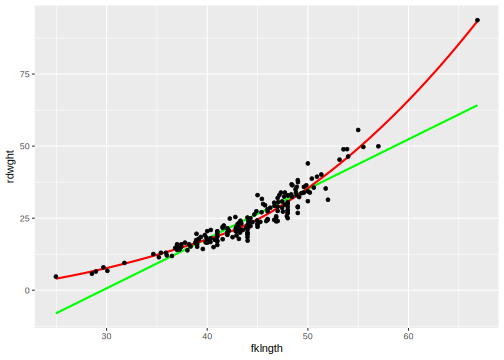
\includegraphics{Labo_BIO4558_files/figure-latex/stur-2-1.pdf}
\caption{\label{fig:stur-2}Graphique du poids en fonction de la longueur des esturgeons}
\end{figure}

\begin{itemize}
\tightlist
\item
  Est-ce que la dispersion des points suggère une bonne corrélation entre les deux variables?
  Est-ce que la relation semble linéaire?
\end{itemize}

Ce graphique suggère une tendance plus curvilinéaire que linéaire.
Malgré tout, il semble y avoir une forte corrélation entre les deux variables.

\begin{itemize}
\tightlist
\item
  Refaites le diagramme de dispersion avec des axes logarithmiques.
\end{itemize}

\begin{Shaded}
\begin{Highlighting}[]
\CommentTok{# apply log transformation on defined graph}
\NormalTok{mygraph }\OperatorTok{+}\StringTok{ }\KeywordTok{scale_x_log10}\NormalTok{() }\OperatorTok{+}\StringTok{ }\KeywordTok{scale_y_log10}\NormalTok{()}
\end{Highlighting}
\end{Shaded}

\begin{figure}
\centering
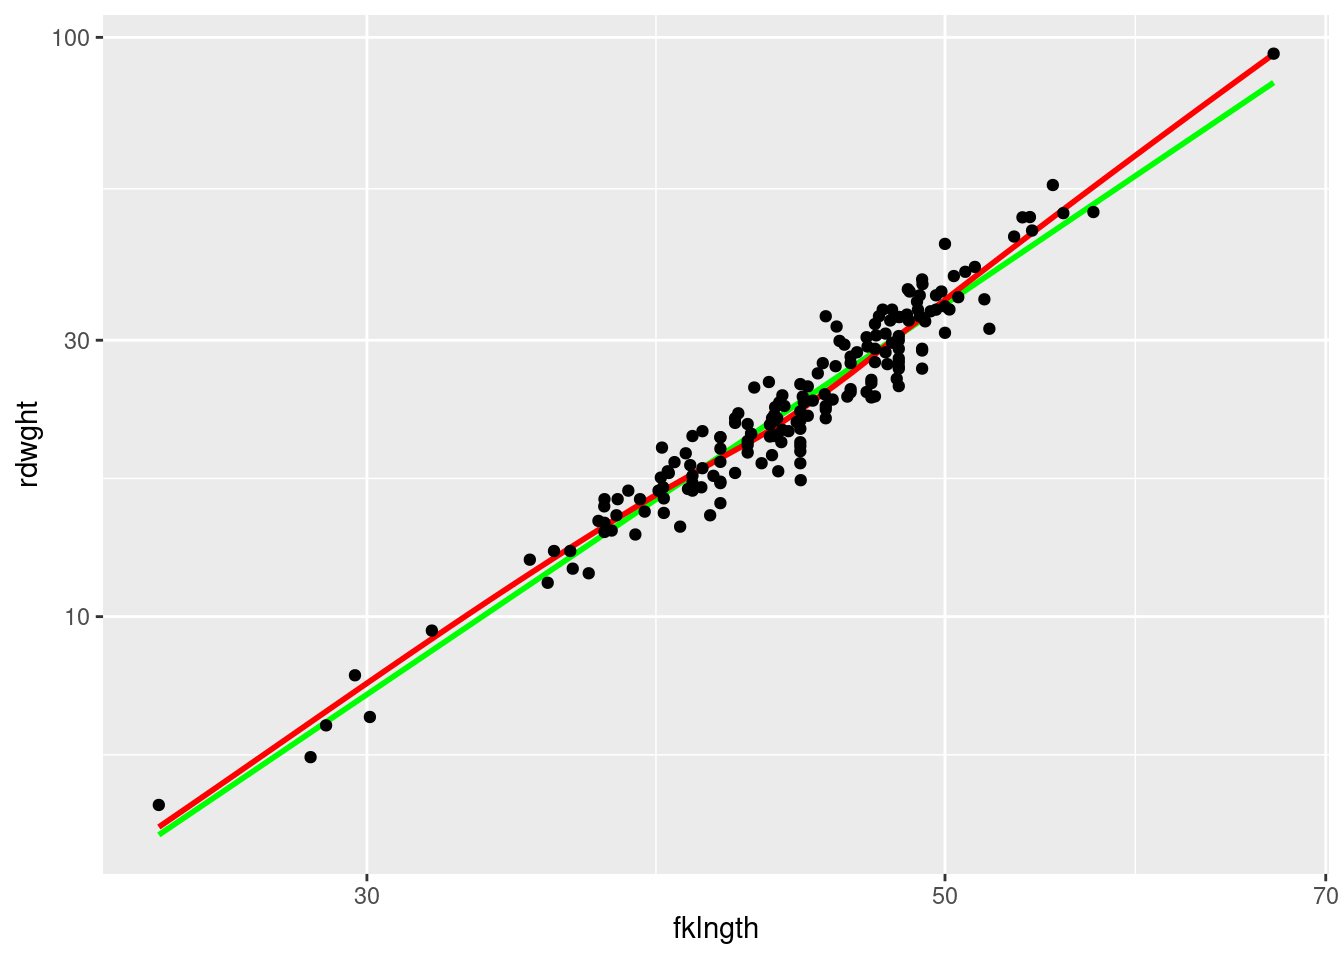
\includegraphics{Labo_BIO4558_files/figure-latex/stur-log-1.pdf}
\caption{\label{fig:stur-log}Graphique poids-longueur avec une échelle log}
\end{figure}

Comparez les diagrammes de dispersion avant et après transformation (Figures \ref{fig:stur-2} et \ref{fig:stur-log}). Comme l'analyse de corrélation présuppose une relation linéaire entre les variables, on devrait donc privilégier l'analyse sur les données log-transformées.

\hypertarget{transformations-et-le-coefficient-de-corruxe9lation}{%
\section{Transformations et le coefficient de corrélation}\label{transformations-et-le-coefficient-de-corruxe9lation}}

Une autre condition préalable à l'analyse de corrélation est que les deux variables concernées suivent une distribution normale bidimensionnelle.
On peut aisément vérifier la normalité de chacune des 2 variables séparément tel que décrit dans le laboratoire précédent.
Si les deux variables sont normalement distribuées, on présume généralement qu'elles suivent une distribution normale bidimensionnelle lorsqu'analysées simultanément (notez que ce n'est pas toujours le cas cependant).

\begin{itemize}
\tightlist
\item
  Examinez la distribution des quatre variables (les deux variables originales et les variables transformées). Que concluez-vous de l'inspection visuelle de ces graphiques ?
\end{itemize}

Les figures ci-dessous sont les diagrammes de probabilité (\texttt{qqplot()}).
Le code pour produire des graphiques multiples sur une page, comme
on voit ci-dessous, est:

\begin{Shaded}
\begin{Highlighting}[]
\KeywordTok{par}\NormalTok{(}\DataTypeTok{mfrow =} \KeywordTok{c}\NormalTok{(}\DecValTok{2}\NormalTok{, }\DecValTok{2}\NormalTok{)) }\CommentTok{# divise le graphique en 4 sections}
\KeywordTok{qqnorm}\NormalTok{(sturgeon}\OperatorTok{$}\NormalTok{fklngth,}\DataTypeTok{ylab=}\StringTok{"fklngth"}\NormalTok{)}
\KeywordTok{qqline}\NormalTok{(sturgeon}\OperatorTok{$}\NormalTok{fklngth)}
\KeywordTok{qqnorm}\NormalTok{(}\KeywordTok{log10}\NormalTok{(sturgeon}\OperatorTok{$}\NormalTok{fklngth),}\DataTypeTok{ylab=}\StringTok{"log10(fklngth)"}\NormalTok{)}
\KeywordTok{qqline}\NormalTok{(}\KeywordTok{log10}\NormalTok{(sturgeon}\OperatorTok{$}\NormalTok{fklngth))}
\KeywordTok{qqnorm}\NormalTok{(sturgeon}\OperatorTok{$}\NormalTok{rdwght,}\DataTypeTok{ylab=}\StringTok{"rdwght"}\NormalTok{)}
\KeywordTok{qqline}\NormalTok{(sturgeon}\OperatorTok{$}\NormalTok{rdwght)}
\KeywordTok{qqnorm}\NormalTok{(}\KeywordTok{log10}\NormalTok{(sturgeon}\OperatorTok{$}\NormalTok{rdwght),}\DataTypeTok{ylab=}\StringTok{"log10(rdwgth)"}\NormalTok{)}
\KeywordTok{qqline}\NormalTok{(}\KeywordTok{log10}\NormalTok{(sturgeon}\OperatorTok{$}\NormalTok{rdwght))}
\end{Highlighting}
\end{Shaded}

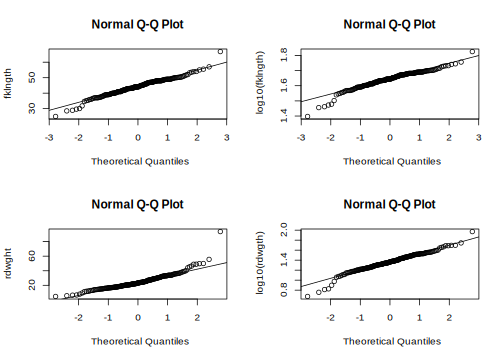
\includegraphics{Labo_BIO4558_files/figure-latex/stur-4hist-1.pdf}

\begin{Shaded}
\begin{Highlighting}[]
\KeywordTok{par}\NormalTok{(}\DataTypeTok{mfrow =} \KeywordTok{c}\NormalTok{(}\DecValTok{1}\NormalTok{, }\DecValTok{1}\NormalTok{)) }\CommentTok{#redéfinie la zone de graphique par défaut}
\end{Highlighting}
\end{Shaded}

Il n'y a pas grand-chose à redire: aucune des distributions n'est
parfaitement normale, mais les déviations semblent mineures.

\begin{itemize}
\tightlist
\item
  Générez une matrice de graphiques de dispersion améliorés en utilisant la commande \texttt{scatterplotMatrix} de la librairie \texttt{car}.
\end{itemize}

\begin{Shaded}
\begin{Highlighting}[]
\KeywordTok{scatterplotMatrix}\NormalTok{(}
  \OperatorTok{~}\NormalTok{fklngth}\OperatorTok{+}\KeywordTok{log10}\NormalTok{(fklngth)}\OperatorTok{+}\NormalTok{rdwght}\OperatorTok{+}\KeywordTok{log10}\NormalTok{(rdwght),}
  \DataTypeTok{data=}\NormalTok{ sturgeon,}
  \DataTypeTok{smooth=}\OtherTok{TRUE}\NormalTok{, }\DataTypeTok{diagonal =} \StringTok{'density'}\NormalTok{)}
\end{Highlighting}
\end{Shaded}

\begin{verbatim}
## Warning in applyDefaults(diagonal, defaults = list(method =
## "adaptiveDensity"), : unnamed diag arguments, will be ignored
\end{verbatim}

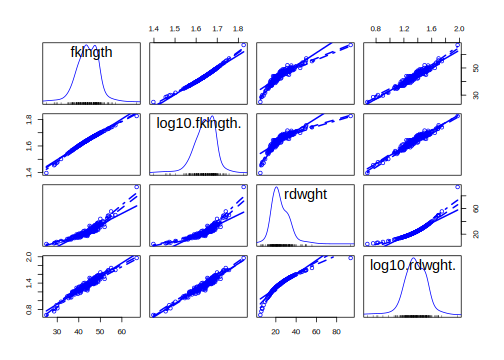
\includegraphics{Labo_BIO4558_files/figure-latex/stur-scatmat-1.pdf}

\begin{itemize}
\tightlist
\item
  Ensuite, calculez le coefficient de corrélation de Pearson entre chaque paire (variables originales et logtransformées ) en utilisant la commande \texttt{cor()}.
  Avant de commencer, on va cependant ajouter les variables transformées au tableau de données sturgeon:
\end{itemize}

\begin{Shaded}
\begin{Highlighting}[]
\NormalTok{sturgeon}\OperatorTok{$}\NormalTok{lfklngth <-}\StringTok{ }\KeywordTok{with}\NormalTok{(sturgeon, }\KeywordTok{log10}\NormalTok{(fklngth))}
\NormalTok{sturgeon}\OperatorTok{$}\NormalTok{lrdwght <-}\StringTok{ }\KeywordTok{log10}\NormalTok{(sturgeon}\OperatorTok{$}\NormalTok{rdwght)}
\end{Highlighting}
\end{Shaded}

Vous pouvez ensuite obtenir la matrice de corrélation par:

\begin{Shaded}
\begin{Highlighting}[]
\KeywordTok{cor}\NormalTok{(sturgeon[,}\KeywordTok{c}\NormalTok{(}\StringTok{"fklngth"}\NormalTok{,}\StringTok{"lfklngth"}\NormalTok{,}\StringTok{"lrdwght"}\NormalTok{,}\StringTok{"rdwght"}\NormalTok{)], }\DataTypeTok{use=}\StringTok{"complete.obs"}\NormalTok{)}
\end{Highlighting}
\end{Shaded}

Fréquemment, il y a des données manquantes dans un échantillon.
En choisissant \texttt{use="complete.obs"}, toutes les lignes du fichier pour lesquelles les variables ne sont pas toutes mesurées sont éliminées.
Dans ce cas, toutes les corrélations seront calculées avec le même nombre de cas.
Par contre, en utilisant \texttt{use="pairwise.complete.obs"} ,
R élimine une observation que lorsqu'un des deux membres de la paire a une valeur manquante.
Dans ce cas, si les données manquantes pour différentes variables se retrouvent dans un groupe différent d'observation, les corrélations ne seront pas nécessairement calculées sur le même nombre de cas ni sur le même sous-ensemble de cas.
En général, vous devriez utiliser l'option \texttt{use="complete.obs"} à moins que vous ayez un très grand nombre de données manquantes et que cette façon de procéder élimine la plus grande partie de vos
observations.

Pourquoi la corrélation entre les variables originales est-elle la plus faible des trois ?

\begin{Shaded}
\begin{Highlighting}[]
\KeywordTok{cor}\NormalTok{(sturgeon[,}\KeywordTok{c}\NormalTok{(}\StringTok{"fklngth"}\NormalTok{,}\StringTok{"lfklngth"}\NormalTok{,}\StringTok{"lrdwght"}\NormalTok{,}\StringTok{"rdwght"}\NormalTok{)], }\DataTypeTok{use=}\StringTok{"complete.obs"}\NormalTok{)}
\end{Highlighting}
\end{Shaded}

\begin{verbatim}
##            fklngth  lfklngth   lrdwght    rdwght
## fklngth  1.0000000 0.9921435 0.9645108 0.9175435
## lfklngth 0.9921435 1.0000000 0.9670139 0.8756203
## lrdwght  0.9645108 0.9670139 1.0000000 0.9265513
## rdwght   0.9175435 0.8756203 0.9265513 1.0000000
\end{verbatim}

Il y a plusieurs choses à noter ici.

\begin{itemize}
\tightlist
\item
  Premièrement, la corrélation entre la longueur à la fourche et le poids rond est élevée, peu importe la transformation: les poissons lourds ont tendance à être longs.
\item
  Deuxièmement, la corrélation est plus forte pour les données
  transformées que pour les données brutes.
\end{itemize}

\textbf{Pourquoi?} Parce que le coefficient de corrélation est inversement proportionnel au bruit autour de la relation linéaire.
Si la relation est curvilinéaire (comme dans le cas des données non transformées), le bruit est plus grand que si la relation est parfaitement linéaire.
Par conséquent, la corrélation est plus faible.

\hypertarget{matrices-de-corruxe9lations-et-correction-de-bonferroni}{%
\section{Matrices de corrélations et correction de Bonferroni}\label{matrices-de-corruxe9lations-et-correction-de-bonferroni}}

Une pratique courante est d'examiner une matrice de corrélation à la recherche des associations significatives.
Comme exemple, essayons de tester si la corrélation entre lfklngth et rdwght est significative (c'est le plus faible coefficient de corrélation de cette matrice).

\begin{itemize}
\tightlist
\item
  Estimer la correlation entre la longueur (fklngth) et le poids (rdwght) des esturgeons:
\end{itemize}

\begin{Shaded}
\begin{Highlighting}[]
\KeywordTok{cor.test}\NormalTok{(}
\NormalTok{  sturgeon}\OperatorTok{$}\NormalTok{lfklngth, sturgeon}\OperatorTok{$}\NormalTok{rdwght,}
  \DataTypeTok{alternative=}\StringTok{"two.sided"}\NormalTok{,}
  \DataTypeTok{method=}\StringTok{"pearson"}\NormalTok{)}
\end{Highlighting}
\end{Shaded}

\begin{verbatim}
## 
## 	Pearson's product-moment correlation
## 
## data:  sturgeon$lfklngth and sturgeon$rdwght
## t = 24.322, df = 180, p-value < 2.2e-16
## alternative hypothesis: true correlation is not equal to 0
## 95 percent confidence interval:
##  0.8367345 0.9057199
## sample estimates:
##       cor 
## 0.8756203
\end{verbatim}

On voit ici que la corrélation est hautement significative (p\textless{} 2.2e-16),ce qui n'est pas surprenant étant donné la valeur du coefficient de corrélation (0.8756).
Il est important de réaliser que si une matrice contient un grand nombre de corrélations, il n'est pas surprenant d'en trouver au moins une qui soit ``significative''.
En effet, on s'attend à en trouver 5\% en moyenne lorsqu'il n'y a en fait aucune corrélation entre les paires de moyennes.
Une façon de corriger pour cette tendance est d'ajuster le niveau \(\alpha\) critique auquel on attribue une signification statistique en divisant \(\alpha\) par le nombre \(k\) de corrélations qui sont examinées : \(\alpha' = \alpha / k\) (ajustement de Bonferroni). Si initialement \(\alpha = 0.05\) et qu'il y a 10 corrélations qui sont examinées, alors \(\alpha'= 0.005\).
Donc, afin de rejeter l'hypothèse nulle, la valeur de p devra être plus petite que \(\alpha'\), en l'occurrence 0.005.
Dans l'exemple qui précède, on devrait donc ajuster \(\alpha\) critique en divisant par le nombre total de corrélations dans la matrice (6 dans ce cas, donc \(\alpha'=0.00833\)).
Cette correction modifie-t-elle votre conclusion quant à la corrélation entre \texttt{lkfl} et \texttt{rdwght}?

\hypertarget{corruxe9lations-non-paramuxe9triques-r-de-spearman-et-tau-de-kendall}{%
\section{Corrélations non paramétriques: r de Spearman et tau de Kendall}\label{corruxe9lations-non-paramuxe9triques-r-de-spearman-et-tau-de-kendall}}

L'analyse faite à la section précédente avec les esturgeons suggère que l'une des conditions préalables à l'analyse de corrélation, soit la distribution normale bidimensionnelle de données, pourrait ne pas être remplie pour \texttt{fklngth} et \texttt{rdwght}, ni pour les paires de variables transformées.
La recherche d'une transformation appropriée peut parfois être difficile.
Pire encore, pour certaines distributions il n'existe pas de transformation qui va normaliser les données.
Dans ces cas-là, la meilleure option est de faire une analyse non
paramétrique qui ne présume ni de la normalité ni de la linéarité.
Ces analyses sont basées sur les rangs.
Les deux plus communes sont le coefficient de rang de Spearman et le tau de Kendall.

\begin{itemize}
\tightlist
\item
  Dans R, testez la corrélation entre \texttt{fklngth} et \texttt{rdwght} en utilisant Spearman et Kendall's .
\end{itemize}

\begin{Shaded}
\begin{Highlighting}[]
\KeywordTok{cor.test}\NormalTok{(}
\NormalTok{  sturgeon}\OperatorTok{$}\NormalTok{lfklngth, sturgeon}\OperatorTok{$}\NormalTok{rdwght,}
  \DataTypeTok{alternative=}\StringTok{"two.sided"}\NormalTok{,}
  \DataTypeTok{method=}\StringTok{"spearman"}\NormalTok{)}
\end{Highlighting}
\end{Shaded}

\begin{verbatim}
## Warning in cor.test.default(sturgeon$lfklngth, sturgeon$rdwght, alternative =
## "two.sided", : Cannot compute exact p-value with ties
\end{verbatim}

\begin{verbatim}
## 
## 	Spearman's rank correlation rho
## 
## data:  sturgeon$lfklngth and sturgeon$rdwght
## S = 47971, p-value < 2.2e-16
## alternative hypothesis: true rho is not equal to 0
## sample estimates:
##       rho 
## 0.9522546
\end{verbatim}

\begin{Shaded}
\begin{Highlighting}[]
\KeywordTok{cor.test}\NormalTok{(}
\NormalTok{  sturgeon}\OperatorTok{$}\NormalTok{lfklngth, sturgeon}\OperatorTok{$}\NormalTok{rdwght,}
  \DataTypeTok{alternative=}\StringTok{"two.sided"}\NormalTok{,}
  \DataTypeTok{method=}\StringTok{"pearson"}\NormalTok{)}
\end{Highlighting}
\end{Shaded}

\begin{verbatim}
## 
## 	Pearson's product-moment correlation
## 
## data:  sturgeon$lfklngth and sturgeon$rdwght
## t = 24.322, df = 180, p-value < 2.2e-16
## alternative hypothesis: true correlation is not equal to 0
## 95 percent confidence interval:
##  0.8367345 0.9057199
## sample estimates:
##       cor 
## 0.8756203
\end{verbatim}

Comparer les résultats de cette analyse à l'analyse paramétrique.
Pourquoi y-a-t'il une différence ?

Calculez les corrélations non paramétriques sur les paires de variables transformées.
Vous devriez voir tout de suite que les corrélations des données transformées et non transformées sont identiques puisque dans les deux cas la corrélation est calculée à partir des rangs qui ne sont pas affectés par la transformation.

Notez que les corrélations obtenues avec le tau de Kendall (0.820) sont plus faibles que celles du coefficient de Spearman (0.952).
Le tau de Kendall pondère un peu plus les grandes différences entre les rangs alors que le coefficient de Spearman donne le même poids à chaque paire d'observations.
En général, on préfère le tau de Kendall lorsqu'il y a plus d'incertitude quant aux rangs qui sont près les uns des autres.

Les esturgeons de cet échantillon ont été capturés à l'aide de filets et d'hameçons d'une taille fixe.
Quel impact cette méthode de capture peut-elle avoir eu sur la forme de la distribution de \texttt{fklngth} et \texttt{rdwght}?
Compte tenu de ces circonstances, l'analyse de corrélation est-elle appropriée ?

Rappelez-vous que l'analyse de corrélation présume aussi que chaque variable est échantillonnée aléatoirement.
Dans le cas de nos esturgeons, ce n'est pas le cas: les hameçons appâtés et les filets ne capturent pas de petits esturgeons (et c'est pourquoi il n'y en a pas dans l'échantillon).
Il faut donc réaliser que les coefficients de corrélation obtenus dans cette analyse ne reflètent pas nécessairement ceux de la population totale des esturgeons.

\hypertarget{ruxe9gression-linuxe9aire-simple}{%
\section{Régression linéaire simple}\label{ruxe9gression-linuxe9aire-simple}}

L'analyse de corrélation vise à décrire comment deux variables covarient.
L'analyse de régression vise plutôt à produire un modèle permettant de prédire une variable (la variable dépendante) par l'autre (la variable indépendante).

Comme pour l'analyse de corrélation, on devrait commencer en examinant des graphiques.
Puisque l'on est intéressé à quantifier la relation entre deux variables, un graphique de la variable dépendante (Y) en fonction de la variable indépendante (X) est tout à fait approprié.

\begin{itemize}
\tightlist
\item
  Le fichier \texttt{sturgeon.csv} contient des données d'un inventaire des esturgeons récoltés en 1978-1980 à Cumberland House en Saskatchewan et à The Pas au Manitoba.
  Faites un diagramme de dispersion de \texttt{fklngth} (la variable dépendante) en fonction de \texttt{age} (la variable indépendante) pour les esturgeons mâles unqiuement et ajoutez-y une régression linéaire et une trace lowess.
  Que concluez-vous de ce diagramme de dispersion ?
\end{itemize}

\begin{Shaded}
\begin{Highlighting}[]
\NormalTok{sturgeon.male <-}\StringTok{ }\KeywordTok{subset}\NormalTok{(sturgeon, }\DataTypeTok{subset =}\NormalTok{ sex }\OperatorTok{==}\StringTok{ "MALE"}\NormalTok{)}
\NormalTok{mygraph <-}\StringTok{ }\KeywordTok{ggplot}\NormalTok{(}
  \DataTypeTok{data=}\NormalTok{sturgeon.male, }\CommentTok{# source of data}
  \KeywordTok{aes}\NormalTok{(}\DataTypeTok{x=}\NormalTok{age, }\DataTypeTok{y=}\NormalTok{fklngth)) }\CommentTok{#aesthetics: y=fklngth, x=rdwght}
\CommentTok{# plot data points, regression, loess trace}
\NormalTok{mygraph <-}\StringTok{ }\NormalTok{mygraph }\OperatorTok{+}
\StringTok{  }\KeywordTok{stat_smooth}\NormalTok{(}\DataTypeTok{method=}\NormalTok{lm, }\DataTypeTok{se=}\OtherTok{FALSE}\NormalTok{, }\DataTypeTok{color=}\StringTok{"green"}\NormalTok{) }\OperatorTok{+}\StringTok{ }\CommentTok{# add linear regression, but no SE shading}
\StringTok{  }\KeywordTok{stat_smooth}\NormalTok{(}\DataTypeTok{color=}\StringTok{"red"}\NormalTok{) }\OperatorTok{+}\StringTok{ }\CommentTok{#add loess}
\StringTok{  }\KeywordTok{geom_point}\NormalTok{() }\CommentTok{# add data points}
\NormalTok{mygraph }\CommentTok{# display graph}
\end{Highlighting}
\end{Shaded}

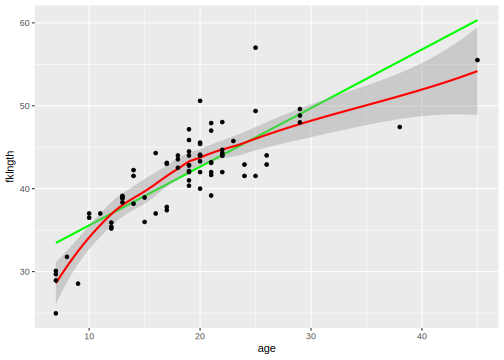
\includegraphics{Labo_BIO4558_files/figure-latex/sturlm-1-1.pdf}

Ce graphique suggère que la relation n'est pas linéaire.

Supposons que nous désirions estimer le taux de croissance des esturgeons mâles.
Un estimé (peut-être pas terrible\ldots{}) du taux de croissance peut être obtenu en calculant la pente de la régression de la longueur à la fourche sur l'âge.

Ajustons d'abord une régression avec la commande lm() et sauvons ces résultats dans un objet appelé \texttt{RegModel.1}.

\begin{Shaded}
\begin{Highlighting}[]
\NormalTok{RegModel}\FloatTok{.1}\NormalTok{ <-}\StringTok{ }\KeywordTok{lm}\NormalTok{(fklngth }\OperatorTok{~}\StringTok{ }\NormalTok{age, }\DataTypeTok{data =}\NormalTok{ sturgeon.male)}
\end{Highlighting}
\end{Shaded}

Rien n'apparait à l'écran, c'est normal ne vous inquiétez pas, tout a été sauvegardé en mémoire.
Pour voir les résultats, tapez:

\begin{Shaded}
\begin{Highlighting}[]
\KeywordTok{summary}\NormalTok{(RegModel}\FloatTok{.1}\NormalTok{)}
\end{Highlighting}
\end{Shaded}

\begin{verbatim}
## 
## Call:
## lm(formula = fklngth ~ age, data = sturgeon.male)
## 
## Residuals:
##     Min      1Q  Median      3Q     Max 
## -8.4936 -2.2263  0.1849  1.7526 10.8234 
## 
## Coefficients:
##             Estimate Std. Error t value Pr(>|t|)    
## (Intercept) 28.50359    1.16873   24.39   <2e-16 ***
## age          0.70724    0.05888   12.01   <2e-16 ***
## ---
## Signif. codes:  0 '***' 0.001 '**' 0.01 '*' 0.05 '.' 0.1 ' ' 1
## 
## Residual standard error: 3.307 on 73 degrees of freedom
##   (5 observations deleted due to missingness)
## Multiple R-squared:  0.664,	Adjusted R-squared:  0.6594 
## F-statistic: 144.3 on 1 and 73 DF,  p-value: < 2.2e-16
\end{verbatim}

\begin{enumerate}
\def\labelenumi{\arabic{enumi}.}
\tightlist
\item
  Le modèle qui a été ajusté et les données utilisées.
\item
  Un sommaire statistique des résidus autour du modèle estimé.
\item
  Valeurs estimées des paramètres du modèle, erreurs-types, statistiques t et probabilités associées.
\item
  Racine carrée de la variance résiduelle.
\item
  Coefficient de détermination. Il correspond à la proportion de la variabilité de la variable dépendante qui peut être expliquée par la régression.
\item
  Le R-carré ajusté tient compte du nombre de paramètres du modèle. Si vous voulez comparer différents modèles qui n'ont pas le même nombre de paramètres, c'est ce qu'il faut utiliser.
\item
  C'est le test de signification omnibus du modèle. Dans le cas de la régression simple, il est équivalent au test sur la pente de la régression.
\end{enumerate}

La régression estimée est donc:

\[ Fklngth = 28.50359 + 0.70724 * age\]

Étant donné la valeur significative du test de F ainsi que pour le test de t pour la pente de la droite, on rejette l'hypothèse nulle qu'il n'y a pas de relation entre la taille et l'âge.

\hypertarget{vuxe9rifier-les-conditions-dapplication-de-la-ruxe9gression}{%
\subsection{Vérifier les conditions d'application de la régression}\label{vuxe9rifier-les-conditions-dapplication-de-la-ruxe9gression}}

La régression simple de type I a quatre conditions préalables :

\begin{enumerate}
\def\labelenumi{\arabic{enumi}.}
\tightlist
\item
  il n'y a pas d'erreur de mesure sur la variable indépendante (X)
\item
  la relation entre Y et X est linéaire
\item
  les résidus sont normalement distribués
\item
  la variance des résidus est constante pour toutes les valeurs de la variable indépendante
\end{enumerate}

Procédons maintenant à l'examen post-mortem. La première
condition est rarement remplie avec des données biologiques ; il y
presque toujours de l'erreur sur X et sur Y. Cela veut dire qu'en
général les pentes estimées sont biaisées, mais que les valeurs prédites
ne le sont pas. Toutefois, si l'erreur de mesure sur X est petite par
rapport à l'étendue des valeurs de X, le résultat de l'analyse n'est pas
dramatiquement influencé. Par contre, si l'erreur de mesure est
relativement grande (toujours par rapport à l'étendue des valeurs de
X), la droite de régression obtenue par la régression de modèle I est
un piètre estimé de la relation fonctionnelle entre X et Y. Dans ce cas,
il est préférable de passer à la régression de modèle II,
malheureusement au-delà du contenu de ce cours.
Les autres conditions préalables à l'analyse de régression de modèle I
peuvent cependant être vérifiées, ou du moins évaluées visuellement.
La commande plot() permet de visualiser des graphiques
diagnostiques pour des modèles linéaires.

\begin{Shaded}
\begin{Highlighting}[]
\KeywordTok{par}\NormalTok{(}\DataTypeTok{mfrow =} \KeywordTok{c}\NormalTok{(}\DecValTok{2}\NormalTok{, }\DecValTok{2}\NormalTok{), }\DataTypeTok{las=}\DecValTok{1}\NormalTok{)}
\KeywordTok{plot}\NormalTok{(RegModel}\FloatTok{.1}\NormalTok{)}
\end{Highlighting}
\end{Shaded}

La commande par() est utilisée pour dire à R de tracer 2 rangées et 2 colonnes de graphiques par page (il y a quatre graphiques diagnostiques qui sont générés automatiquement pour les modèles linéaires), et la commande las indique à R d'effectuer une rotation des légendes de l'axe des Y pour qu'elles soient perpendiculaires à l'axe (oui. Je sais. Rien de tout ça n'est évident.)

Vous obtiendrez:
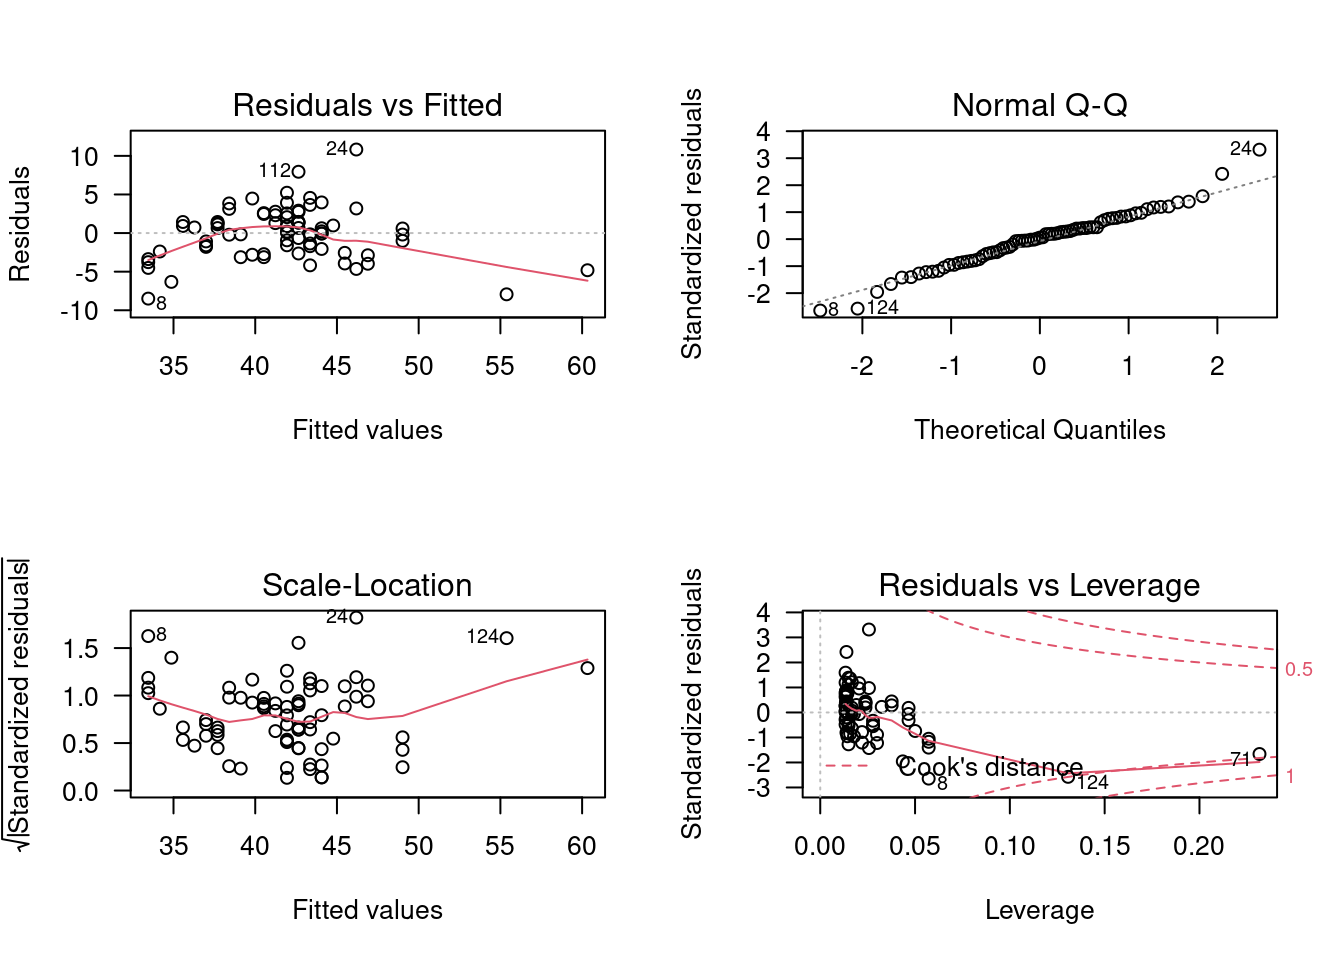
\includegraphics{Labo_BIO4558_files/figure-latex/sturlmv-1eval-1.pdf}

\begin{enumerate}
\def\labelenumi{\arabic{enumi}.}
\tightlist
\item
  En haut à gauche, permet d'évaluer la linéarité, la normalité, et l'homoscédasticité des résidus. Il illustre les déviations autour de la régression en fonction des valeurs prédites. Rappllez-vous que le graphique de fklngth vs age suggère que la relation entre la longueur à la fourche et l'âge n'est pas linéaire. Les très jeunes et très vieux esturgeons sont sous la droite en général, alors que les esturgeons d'âge moyen sont retrouvés généralement au-dessus de la droite de régression. C'est exactement ce que le graphique des résidus en fonction des valeurs prédites illustre. La ligne en rouge est une trace lowess au travers de ce nuage de points. Si la relation était linéaire, la trace lowess serait presque plate et près de 0. La dispersion des résidus permet d'évaluer visuellement leur normalité et hétéroscédasticité; mais ce graphique n'est pas optimal pour évaluer ces propriétés. Les deux graphiques suivants sont supérieurs au premier pour cela.
\item
  En haut à droite permet d'évaluer la normalité des résidus. C'est un graphique QQ des résidus (QQ plot). Des résidus distribués normalement tomberaient exactement sur la diagonale. Ici, on voit que c'est presque le cas, sauf dans les queues de la distribution.
\item
  En bas à gauche, intitulé Scale-Location, permet d'évaluer l'homoscedasticité. On y retrouve sur l'ordonnée (l'axe des y) la racine carrée de la valeur absolue des résidus standardisés (résidus divisés par l'écart-type des résidus) en fonction des valeurs prédites. Le graphique aide à déterminer si la variation des résidus est constante ou non. Si les résidus sont homoscédastiques, la valeur moyenne sur l'axe des y ne va pas changer en fonction de la valeur prédite. Ici, il y a une certaine tendance, mais pas une tendance monotone puisqu' il y a d'abord une baisse puis une hausse..; bref, rien qui soit une forte évidence contre la supposition d'homoscédasticité.
\item
  En bas à droite, montre les résidus en fonction du ``leverage'' et permet de détecter certaines valeurs extrêmes qui ont une grande influence sur la régression. Le leverage d'un point mesure sa distance des autres points, mais seulement en ce qui concerne les variables indépendantes. Dans le cas d'une régression simple, cela revient à la distance entre le point sur l'axe des x et la moyenne de tous les points sur cet axe. Vous devriez porter une attention particulière aux observations qui ont un leverage plus grand que \(2(k+1)/n\), où k est le nombre de variables indépendantes (ici, 1) et n est le nombre d'observations. Dans cet exemple, il y a 75 observations et une variable indépendante et donc les points ayant un leverage plus grand que \(4 / 75 = 0.053\) devrait être considérés avec attention. Le graphique indique également comment la régression changerait si on enlevait un point. Ce changement est mesuré par la distance de Cook, illustrée par les bandes en rouge sur le graphique. Un point ayant une distance de Cook supérieure à 1 a une grande influence.
\end{enumerate}

\begin{rmdwarning}
Notez que R identifie automatiquement les cas les plus extrèmes sur chacun de ces 4 graphiques. Le fait qu'un point soit identifié ne signifie pas nécessairement que c'est une valeur réellement extrème, ou que vous devez vous en préoccuper. Dans tous les ensembles de données il y aura toujours un résidu plus grand que les autres\ldots{}
\end{rmdwarning}

Finalement, quel est le verdict concernant la régression linéaire entre fklngth et age ? Elle viole la condition de linéarité, possiblement celle de normalité, remplit la condition d'homoscédasticité, et ne semble pas influencée outre mesure par des valeurs bizarres ou extrêmes.

\hypertarget{tests-formels-des-conditions-dapplication-pour-la-ruxe9gression}{%
\subsection{Tests formels des conditions d'application pour la régression}\label{tests-formels-des-conditions-dapplication-pour-la-ruxe9gression}}

Personnellement, je n'utilise jamais les tests formels des conditions d'application de la régression et me contente des graphiques des résidus pour guider mes décisions. C'est ce que la plupart des praticiens font. Cependant, lors de mes premières analyses, je n'étais pas toujours certain de bien interpréter les graphiques et j'aurais aimé un indice plus formel ou un test permettant de détecter les violations des conditions d'application de la régression.

Le package \texttt{lmtest} , qui ne fait pas partie de l'installation de base, mais qui est disponible sur CRAN, permet de faire plusieurs tests de linéarité et d'homoscédasticité. Et on peut tester la normalité avec le test Shapiro-Wilk test vu précédemment.

\begin{rmdcode}
Charger le package lmtest de CRAN (et installer le si besoin).
\end{rmdcode}

\begin{Shaded}
\begin{Highlighting}[]
\KeywordTok{library}\NormalTok{(lmtest)}
\end{Highlighting}
\end{Shaded}

\begin{rmdcode}
Exécutez les commandes suivantes
\end{rmdcode}

\begin{Shaded}
\begin{Highlighting}[]
\KeywordTok{bptest}\NormalTok{(RegModel}\FloatTok{.1}\NormalTok{)}
\end{Highlighting}
\end{Shaded}

\begin{verbatim}
## 
## 	studentized Breusch-Pagan test
## 
## data:  RegModel.1
## BP = 1.1765, df = 1, p-value = 0.2781
\end{verbatim}

Le test Breusch-Pagan test examine si la variabilité des résidus est constantes lorsque les valeurs prédites changent. Une faible valeur de p suggère de l'hétéroscédasticité. Ici, la valeur p est élevée et suggère que la condition d'application d'homoscédasticité est remplie avec ces données.

\begin{Shaded}
\begin{Highlighting}[]
\KeywordTok{dwtest}\NormalTok{(RegModel}\FloatTok{.1}\NormalTok{)}
\end{Highlighting}
\end{Shaded}

\begin{verbatim}
## 
## 	Durbin-Watson test
## 
## data:  RegModel.1
## DW = 2.242, p-value = 0.8489
## alternative hypothesis: true autocorrelation is greater than 0
\end{verbatim}

Le test Durbin-Watson permet de détecter l'autocorrélation sérielle des résidus. En l'absence d'autocorrélation (i.e.~d'indépendance des résidus) la valeur attendue de la statistique D est 2. Ce test permet d'éprouver l'hypothèse d'indépendance des résidus, mais ne permet de détecter qu'un type particulier de dépendance. Ici, le test ne permet pas de rejeter l'hypothèse d'indépendance.

\begin{Shaded}
\begin{Highlighting}[]
\KeywordTok{resettest}\NormalTok{(RegModel}\FloatTok{.1}\NormalTok{)}
\end{Highlighting}
\end{Shaded}

\begin{verbatim}
## 
## 	RESET test
## 
## data:  RegModel.1
## RESET = 14.544, df1 = 2, df2 = 71, p-value = 5.082e-06
\end{verbatim}

Le test RESET permet d'éprouver la linéarité. Si la relation est linéaire, alors la statistique RESET sera d'environ 1. Ici, la statistique est beaucoup plus élevée (14.54) et hautement significative. Le test confirme la tendance que nous avons détectée visuellement plus haut: la relation n'est pas linéaire.

\begin{Shaded}
\begin{Highlighting}[]
\KeywordTok{shapiro.test}\NormalTok{(}\KeywordTok{residuals}\NormalTok{(RegModel}\FloatTok{.1}\NormalTok{))}
\end{Highlighting}
\end{Shaded}

\begin{verbatim}
## 
## 	Shapiro-Wilk normality test
## 
## data:  residuals(RegModel.1)
## W = 0.98037, p-value = 0.2961
\end{verbatim}

Le test de normalité Shapiro-Wilk sur les résidus confirme que la déviation par rapport à une distribution normale des résidus n'est pas grande.

\hypertarget{transformation-des-donnuxe9es-en-ruxe9gression}{%
\section{Transformation des données en régression}\label{transformation-des-donnuxe9es-en-ruxe9gression}}

La relation entre \texttt{fklngth} et \texttt{age} n'étant pas linéaire, on devrait donc essayer de transformer les données pour tenter de les linéariser :

\begin{itemize}
\tightlist
\item
  Voyons ce qu'une transformation log donne:
\end{itemize}

\begin{Shaded}
\begin{Highlighting}[]
\KeywordTok{par}\NormalTok{(}\DataTypeTok{mfrow =} \KeywordTok{c}\NormalTok{(}\DecValTok{1}\NormalTok{, }\DecValTok{1}\NormalTok{), }\DataTypeTok{las=}\DecValTok{1}\NormalTok{)}
\KeywordTok{ggplot}\NormalTok{(}
  \DataTypeTok{data =}\NormalTok{ sturgeon.male,}
  \KeywordTok{aes}\NormalTok{(}\DataTypeTok{x=}\KeywordTok{log10}\NormalTok{(age), }\DataTypeTok{y=}\KeywordTok{log10}\NormalTok{(fklngth))) }\OperatorTok{+}
\StringTok{  }\KeywordTok{geom_smooth}\NormalTok{(}\DataTypeTok{color=}\StringTok{"red"}\NormalTok{)}\OperatorTok{+}
\StringTok{  }\KeywordTok{geom_smooth}\NormalTok{(}\DataTypeTok{method=}\StringTok{"lm"}\NormalTok{, }\DataTypeTok{se=}\OtherTok{FALSE}\NormalTok{, }\DataTypeTok{color=}\StringTok{"green"}\NormalTok{)}\OperatorTok{+}
\StringTok{  }\KeywordTok{geom_point}\NormalTok{()}
\end{Highlighting}
\end{Shaded}

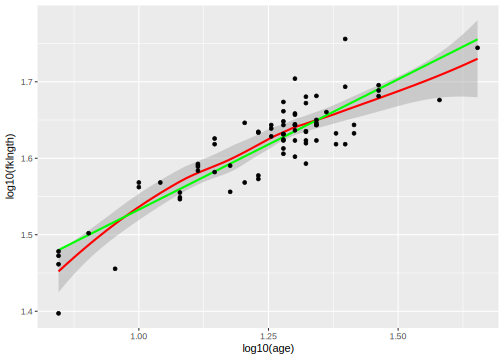
\includegraphics{Labo_BIO4558_files/figure-latex/sturtr-1-1.pdf}

Ajustons maintenant une régression simple sur ces données transformées.

\begin{Shaded}
\begin{Highlighting}[]
\NormalTok{RegModel}\FloatTok{.2}\NormalTok{ <-}\StringTok{ }\KeywordTok{lm}\NormalTok{(}\KeywordTok{log10}\NormalTok{(fklngth)}\OperatorTok{~}\KeywordTok{log10}\NormalTok{(age), }\DataTypeTok{data=}\NormalTok{sturgeon.male)}
\KeywordTok{summary}\NormalTok{(RegModel}\FloatTok{.2}\NormalTok{)}
\end{Highlighting}
\end{Shaded}

\begin{verbatim}
## 
## Call:
## lm(formula = log10(fklngth) ~ log10(age), data = sturgeon.male)
## 
## Residuals:
##       Min        1Q    Median        3Q       Max 
## -0.082794 -0.016837 -0.000719  0.021102  0.087446 
## 
## Coefficients:
##             Estimate Std. Error t value Pr(>|t|)    
## (Intercept)  1.19199    0.02723   43.77   <2e-16 ***
## log10(age)   0.34086    0.02168   15.72   <2e-16 ***
## ---
## Signif. codes:  0 '***' 0.001 '**' 0.01 '*' 0.05 '.' 0.1 ' ' 1
## 
## Residual standard error: 0.03015 on 73 degrees of freedom
##   (5 observations deleted due to missingness)
## Multiple R-squared:  0.772,	Adjusted R-squared:  0.7688 
## F-statistic: 247.1 on 1 and 73 DF,  p-value: < 2.2e-16
\end{verbatim}

Examinons maintenant les graphiques diagnostiques:

\begin{Shaded}
\begin{Highlighting}[]
\KeywordTok{par}\NormalTok{(}\DataTypeTok{mfrow =} \KeywordTok{c}\NormalTok{(}\DecValTok{2}\NormalTok{, }\DecValTok{2}\NormalTok{), }\DataTypeTok{las=}\DecValTok{1}\NormalTok{)}
\KeywordTok{plot}\NormalTok{(RegModel}\FloatTok{.2}\NormalTok{)}
\end{Highlighting}
\end{Shaded}

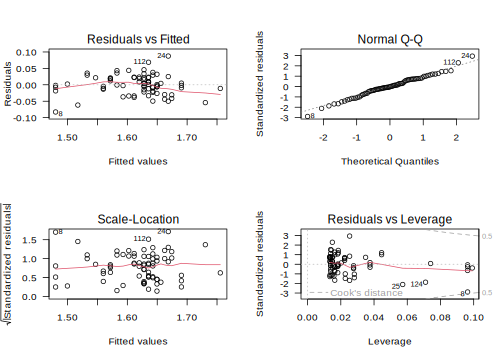
\includegraphics{Labo_BIO4558_files/figure-latex/sturtr-3-1.pdf}

Il y a une certaine amélioration, mais ce n'est pas encore parfait (la perfection n'est pas de ce monde\ldots{}.). Le graphique des résidus en fonction des valeurs prédites suggère encore une certaine non linéarité. Sur le graphique Q-Q les points se retrouvent plus près de la droite diagonale qu'avant, indiquant que les résidus sont encore plus près de la normalité après la transformation log-log. Il n'y a pas d'indice d'hétéroscédasticité. Finalement, même si il reste quelques points avec plus d'influence (leverage) que les autres, aucun n'a une distance de Cook au-delà de 0.5. En résumé, la transformation log a amélioré les choses: relation est plus linéaire, les résidus sont plus normaux, et il y a moins de points avec une influence relativement élevée.Est-ce que les tests formels supportent cette évaluation?

\begin{Shaded}
\begin{Highlighting}[]
\KeywordTok{bptest}\NormalTok{(RegModel}\FloatTok{.2}\NormalTok{)}
\end{Highlighting}
\end{Shaded}

\begin{verbatim}
## 
## 	studentized Breusch-Pagan test
## 
## data:  RegModel.2
## BP = 0.14282, df = 1, p-value = 0.7055
\end{verbatim}

\begin{Shaded}
\begin{Highlighting}[]
\KeywordTok{dwtest}\NormalTok{(RegModel}\FloatTok{.2}\NormalTok{)}
\end{Highlighting}
\end{Shaded}

\begin{verbatim}
## 
## 	Durbin-Watson test
## 
## data:  RegModel.2
## DW = 2.1777, p-value = 0.6134
## alternative hypothesis: true autocorrelation is greater than 0
\end{verbatim}

\begin{Shaded}
\begin{Highlighting}[]
\KeywordTok{resettest}\NormalTok{(RegModel}\FloatTok{.2}\NormalTok{)}
\end{Highlighting}
\end{Shaded}

\begin{verbatim}
## 
## 	RESET test
## 
## data:  RegModel.2
## RESET = 4.4413, df1 = 2, df2 = 71, p-value = 0.01523
\end{verbatim}

\begin{Shaded}
\begin{Highlighting}[]
\KeywordTok{shapiro.test}\NormalTok{(}\KeywordTok{residuals}\NormalTok{(RegModel}\FloatTok{.2}\NormalTok{))}
\end{Highlighting}
\end{Shaded}

\begin{verbatim}
## 
## 	Shapiro-Wilk normality test
## 
## data:  residuals(RegModel.2)
## W = 0.98998, p-value = 0.8246
\end{verbatim}

Oui, les conclusions sont les mêmes: les résidus sont encore homoscédastiques (test Breusch-Pagan), ne sont pas autocorrélés (test Durbin-Watson), sont normaux (test Shapiro-Wilk ), et sont plus linéaires (la valeur de P du test RESET est maintenant 0.015, au lieu de 0.000005). Donc la linéarité a augmenté, mais cette condition d'application semble encore légèrement violée.

\hypertarget{traitement-des-valeurs-extruxe8mes}{%
\section{Traitement des valeurs extrèmes}\label{traitement-des-valeurs-extruxe8mes}}

Dans cet exemple, il n'y a pas de valeur vraiment extrème. Oui, je sais, R a quand même identifié les observations 8, 24, et 112 dans le dernier graphique diagnostique. Mais ces valeurs sont encore dans la fourchette de valeurs que je juge ``acceptables''. Mais comment déterminer objectivement ce qui est acceptable? À quel moment juge t'on qu'une valeur extrême est vraiment trop invraisemblable pour ne pas l'exclure? Il n'y a malheureusement pas de règle absolue là-dessus. Les opinions varient, mais je penche vers le conservatisme sur cette question.

Ma position est que, à moins que la valeur soit biologiquement impossible ou clairement une erreur d'entrée de données, je n'élimine pas les valeurs extrêmes et j'utilise toutes mes données dans leur analyse. Pourquoi?

Parce que je veux que mes données reflètent bien la variabilité naturelle ou réelle. C'est d'ailleurs parfois cette variabilité qui est intéressante.

L'approche conservatrice qui consiste à conserver toutes les valeurs extrêmes possibles est possiblement la plus honnête, mais elle peut causer certains problèmes. Ces valeurs extrêmes sont souvent la cause des violations des conditions d'application des tests statistiques. La solution suggérée à ce dilemme est de faire l'analyse avec et sans les valeurs extrêmes et de comparer les conclusions. Dans bien des cas, les conclusions seront qualitativement les mêmes et les tailles d'effet ne seront pas très différentes. Toutefois, dans certains cas, la présence des valeurs extrêmes change complètement les conclusions. Dans ces cas, il faut simplement accepter que les conclusions dépendent entièrement de la présence des valeurs extrêmes et sont donc peu concluantes.

Suivant cette approche comparative, refaisons donc l'analyse après
avoir enlevé les observations 8, 24, et 112.

\begin{Shaded}
\begin{Highlighting}[]
\NormalTok{RegModel}\FloatTok{.3}\NormalTok{ <-}\StringTok{ }\KeywordTok{lm}\NormalTok{(}\KeywordTok{log10}\NormalTok{(fklngth)}\OperatorTok{~}\KeywordTok{log10}\NormalTok{(age), }\DataTypeTok{data=}\NormalTok{sturgeon.male, }\DataTypeTok{subset =} \OperatorTok{!}\NormalTok{(}\KeywordTok{rownames}\NormalTok{(sturgeon.male) }\OperatorTok\StringTok{ }\KeywordTok{c}\NormalTok{(}\StringTok{'8'}\NormalTok{,}\StringTok{'24'}\NormalTok{,}\StringTok{'112'}\NormalTok{)))}
\KeywordTok{summary}\NormalTok{(RegModel}\FloatTok{.3}\NormalTok{)}
\end{Highlighting}
\end{Shaded}

\begin{verbatim}
## 
## Call:
## lm(formula = log10(fklngth) ~ log10(age), data = sturgeon.male, 
##     subset = !(rownames(sturgeon.male) %in% c("8", "24", "112")))
## 
## Residuals:
##       Min        1Q    Median        3Q       Max 
## -0.069163 -0.017390  0.000986  0.018590  0.047647 
## 
## Coefficients:
##             Estimate Std. Error t value Pr(>|t|)    
## (Intercept)  1.22676    0.02431   50.46   <2e-16 ***
## log10(age)   0.31219    0.01932   16.16   <2e-16 ***
## ---
## Signif. codes:  0 '***' 0.001 '**' 0.01 '*' 0.05 '.' 0.1 ' ' 1
## 
## Residual standard error: 0.02554 on 70 degrees of freedom
##   (5 observations deleted due to missingness)
## Multiple R-squared:  0.7885,	Adjusted R-squared:  0.7855 
## F-statistic:   261 on 1 and 70 DF,  p-value: < 2.2e-16
\end{verbatim}

L'ordonnée à l'origine (Intercept), la pente, et le R carré sont presque les mêmes, et la valeur de p est encore astronomiquement petite. Enlever les valeurs extrêmes a peu d'effet dans ce cas.

Les graphiques diagnostiques des résidus et les tests formels des conditions d'application sur ce sous-ensemble de données donnent:

\begin{Shaded}
\begin{Highlighting}[]
\KeywordTok{par}\NormalTok{(}\DataTypeTok{mfrow =} \KeywordTok{c}\NormalTok{(}\DecValTok{2}\NormalTok{,}\DecValTok{2}\NormalTok{))}
\KeywordTok{plot}\NormalTok{(RegModel}\FloatTok{.3}\NormalTok{)}
\end{Highlighting}
\end{Shaded}

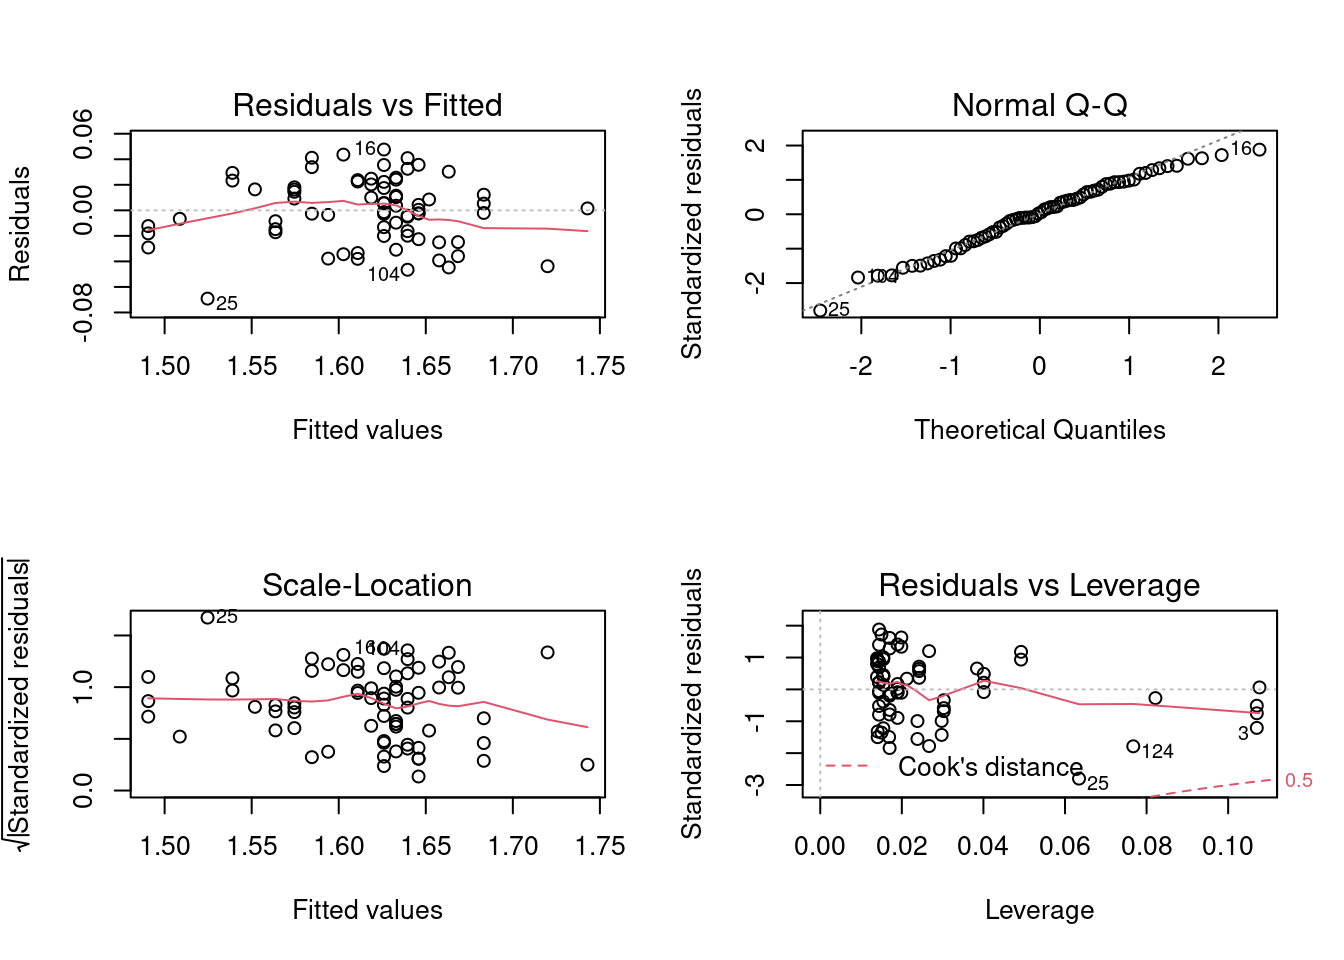
\includegraphics{Labo_BIO4558_files/figure-latex/sturtr-6-1.pdf}

\begin{Shaded}
\begin{Highlighting}[]
\NormalTok{sturgeon.male.subset <-}\StringTok{ }\KeywordTok{subset}\NormalTok{(sturgeon, }\DataTypeTok{subset=}\OperatorTok{!}\NormalTok{(}\KeywordTok{rownames}\NormalTok{(sturgeon.male) }\OperatorTok\StringTok{ }\KeywordTok{c}\NormalTok{(}\StringTok{'8'}\NormalTok{,}\StringTok{'24'}\NormalTok{,}\StringTok{'112'}\NormalTok{)))}
\KeywordTok{bptest}\NormalTok{(RegModel}\FloatTok{.3}\NormalTok{)}
\end{Highlighting}
\end{Shaded}

\begin{verbatim}
## 
## 	studentized Breusch-Pagan test
## 
## data:  RegModel.3
## BP = 0.3001, df = 1, p-value = 0.5838
\end{verbatim}

\begin{Shaded}
\begin{Highlighting}[]
\KeywordTok{dwtest}\NormalTok{(RegModel}\FloatTok{.3}\NormalTok{)}
\end{Highlighting}
\end{Shaded}

\begin{verbatim}
## 
## 	Durbin-Watson test
## 
## data:  RegModel.3
## DW = 2.0171, p-value = 0.5074
## alternative hypothesis: true autocorrelation is greater than 0
\end{verbatim}

\begin{Shaded}
\begin{Highlighting}[]
\KeywordTok{resettest}\NormalTok{(RegModel}\FloatTok{.3}\NormalTok{)}
\end{Highlighting}
\end{Shaded}

\begin{verbatim}
## 
## 	RESET test
## 
## data:  RegModel.3
## RESET = 3.407, df1 = 2, df2 = 68, p-value = 0.0389
\end{verbatim}

\begin{Shaded}
\begin{Highlighting}[]
\KeywordTok{shapiro.test}\NormalTok{(}\KeywordTok{residuals}\NormalTok{(RegModel}\FloatTok{.3}\NormalTok{))}
\end{Highlighting}
\end{Shaded}

\begin{verbatim}
## 
## 	Shapiro-Wilk normality test
## 
## data:  residuals(RegModel.3)
## W = 0.98318, p-value = 0.4502
\end{verbatim}

Il n'y a pas vraiment de différence ici non plus avec l'analyse des données en entier. Bref, tout pointe vers la conclusion que les valeurs les plus extrêmes de cet ensemble de donnée n'influencent pas indûment les résultats statistiques.

\hypertarget{quantifier-la-taille-deffet-et-analyse-de-puissance-en-ruxe9gression}{%
\section{Quantifier la taille d'effet et analyse de puissance en régression}\label{quantifier-la-taille-deffet-et-analyse-de-puissance-en-ruxe9gression}}

L'interprétation biologique des résultats n'est pas la même chose que l'interprétation statistique. Dans l'analyse qui précède, on conclue statistiquement que la taille augmente avec l'âge (puisque la pente est positive et et p\textless{}0.05). Mais cette augmentation ``statistique'' de la taille avec l'âge ne donne pas d'information sur la différence de taille entre les jeunes et vieux individus. La pente et un graphique sont plus informatifs à ce sujet que la valeur p.~La pente (dans l'espace log-log) est 0.34. Cela veut dire que pour chaque unité d'accroissement de X (log10(age)), il y a une augmentation de 0.34 unités de log10(fklngth). En d'autres mots, quand l'âge est multiplié par 10, la longueur à la fourche est multipliée environ par 2. Donc la longueur des esturgeons augmente plus lentement que leur âge (contrairement à mon tour de taille, semble-t-il\ldots{}.). La valeur de la pente (0.34) est un estimé de la taille de l'effet de l'âge sur la longueur.

\hypertarget{puissance-de-duxe9tecter-une-pente-donnuxe9e}{%
\subsection{Puissance de détecter une pente donnée}\label{puissance-de-duxe9tecter-une-pente-donnuxe9e}}

Pour les calculs de puissance avec G*Power vous devrez cependant utiliser une autre métrique de la taille de l'effet, calculée à partir de la pente, de son erreur-type, et de la taille de l'échantillon (ce qui facilite les calculs pour G*Power, mais malheureusement pas pour vous ;-) La métrique (d) est calculée comme:
\[ d = \frac{b}{s_b\sqrt{n-k-1}} \]
où \(b\) est l'estimé de la pente, \(s_b\) est l'erreur type de la pente, \(n\) est le nombre d'observations, et \(k\) est le nombre de variables indépendantes (1 pour la régression linéaire simple).

Vous pouvez calculer approximativement la puissance avec G*Power pour une valeur de pente que vous jugez assez grande pour mériter d'être détectée. Allez à \textbf{Tests: Means: One group: difference from constant}, là, vous devrez remplacer la valeur de \(b\) dans l'équation pour la taille d'effet (d) par la pente que vous voudriez détecter, mais utiliser l'erreur type calculée à partir de vos données.

Par exemple, supposons que les ichthyologues considèrent qu'une pente de 0.1 pour la relation entre log10(fklngth) et log10(age) est signifiante biologiquement, et qu'ils désirent estimer la puissance de détecter une telle pente à partir d'un échantillon de 20 esturgeons. Les résultats de la régression log-log nous fournissent ce dont on a besoin:

\begin{Shaded}
\begin{Highlighting}[]
\KeywordTok{summary}\NormalTok{(RegModel}\FloatTok{.2}\NormalTok{)}
\end{Highlighting}
\end{Shaded}

\begin{verbatim}
## 
## Call:
## lm(formula = log10(fklngth) ~ log10(age), data = sturgeon.male)
## 
## Residuals:
##       Min        1Q    Median        3Q       Max 
## -0.082794 -0.016837 -0.000719  0.021102  0.087446 
## 
## Coefficients:
##             Estimate Std. Error t value Pr(>|t|)    
## (Intercept)  1.19199    0.02723   43.77   <2e-16 ***
## log10(age)   0.34086    0.02168   15.72   <2e-16 ***
## ---
## Signif. codes:  0 '***' 0.001 '**' 0.01 '*' 0.05 '.' 0.1 ' ' 1
## 
## Residual standard error: 0.03015 on 73 degrees of freedom
##   (5 observations deleted due to missingness)
## Multiple R-squared:  0.772,	Adjusted R-squared:  0.7688 
## F-statistic: 247.1 on 1 and 73 DF,  p-value: < 2.2e-16
\end{verbatim}

L'erreur-type de la pente est 0.02168. Il y avait 75 poissons (n=75) dans l'échantillon de départ. On peut donc calculer la métrique de taille d'effet pour G*Power
\[ d = \frac{b}{s_b\sqrt{n-k-1}} = \frac{0.1}{0.02168\sqrt{74-1-1}}=0.54\]

Armés de cette taille d'effet (une pente présumée de 0.1 et une variabilité autour de la régression similaire à la régression de fklngth vs age), aller à \textbf{Tests: Means: One group: difference from constant}, et entrez la valeur calculée de d, alpha, et l'effectif de l'échantillon pour calculer la puissance.

\begin{figure}

\includegraphics[width=1\linewidth]{images/lm_pow_1} \caption{Analyse de puissance pour N = 20 et pente = 0.1}\label{fig:lm-pow-fig-1}
\end{figure}

La puissance de détecter une pente comme étant statistiquement significative (au niveau alpha), si la pente est 0.1, que la variabilité résiduelle autour de la régression est semblable à celle de notre échantillon (ce qui revient à une taille d'effet de 0.54, pour un échantillon de 20 esturgeons et alpha=0.05) est de 0.629. Seulement environ 2/3 des échantillons de cette taille détecteraient un effet significatif de l'âge sur \texttt{fklngth}.

\hypertarget{effectif-requis-pour-atteindre-une-puissance-duxe9siruxe9e-test-a-priori}{%
\subsection{Effectif requis pour atteindre une puissance désirée (test A-priori)}\label{effectif-requis-pour-atteindre-une-puissance-duxe9siruxe9e-test-a-priori}}

Pour estimer la taille d'échantillon (effectif) requis pour avoir une puissance de 99\% de détecter un effet de l'âge si la pente est 0.1 (sur une échelle log-log ), avec alpha=0.05, on utilise la même valeur de d (0.54):

\begin{figure}

\includegraphics[width=1\linewidth]{images/lm_pow_2} \caption{Analyse à priori pour déterminer la taille d'échantillon pour une puissance de 0.99}\label{fig:lm-pow-fig-2}
\end{figure}

En augmentant la taille de l'échantillon à 65, selon le même scénario que précédemment, la puissance augmente à 99\%.

\hypertarget{bootstrap-en-ruxe9gression-simple-avec-r}{%
\section{Bootstrap en régression simple avec R}\label{bootstrap-en-ruxe9gression-simple-avec-r}}

Un test non paramétrique pour l'ordonnée à l'origine et la pente d'une régression simple peut être effectué par bootstrap.

\begin{Shaded}
\begin{Highlighting}[]
\CommentTok{#charger le paquet boot}
\KeywordTok{library}\NormalTok{(boot)}
\CommentTok{# obtenir les poids de régression}
\NormalTok{bs <-}\StringTok{ }\ControlFlowTok{function}\NormalTok{(formula, data, indices) \{}
\NormalTok{  d <-}\StringTok{ }\NormalTok{data[indices,] }\CommentTok{# allows boot to select sample}
\NormalTok{  fit <-}\StringTok{ }\KeywordTok{lm}\NormalTok{(formula, }\DataTypeTok{data =}\NormalTok{ d)}
  \KeywordTok{return}\NormalTok{(}\KeywordTok{coef}\NormalTok{(fit))}
\NormalTok{\}}
\CommentTok{# bootstrapping with 1000 replications}
\NormalTok{results <-}\StringTok{ }\KeywordTok{boot}\NormalTok{(}
  \DataTypeTok{data =}\NormalTok{ sturgeon.male,}
  \DataTypeTok{statistic =}\NormalTok{ bs,}
  \DataTypeTok{R=}\DecValTok{1000}\NormalTok{, }\DataTypeTok{formula=}\KeywordTok{log10}\NormalTok{(fklngth)}\OperatorTok{~}\KeywordTok{log10}\NormalTok{(age))}
\CommentTok{# view results}
\NormalTok{results}
\end{Highlighting}
\end{Shaded}

\begin{verbatim}
## 
## ORDINARY NONPARAMETRIC BOOTSTRAP
## 
## 
## Call:
## boot(data = sturgeon.male, statistic = bs, R = 1000, formula = log10(fklngth) ~ 
##     log10(age))
## 
## 
## Bootstrap Statistics :
##      original       bias    std. error
## t1* 1.1919926  0.001817578  0.03382908
## t2* 0.3408557 -0.001411900  0.02680257
\end{verbatim}

Pour chaque paramètre du modèle (ici l'ordonnée à l'origine est
appelée t1* et la pente de la régression t2*), R imprime :

\begin{enumerate}
\def\labelenumi{\arabic{enumi}.}
\tightlist
\item
  \texttt{original} la valeur estimée sur tout l'échantillon
\item
  \texttt{bias} la différence entre la valeur moyenne des estimés par bootstrap et la valeur originale sur tout l'échantillon
\item
  \texttt{std.\ error} l'erreur-type de l'estimé bootstrap
\end{enumerate}

\begin{Shaded}
\begin{Highlighting}[]
\KeywordTok{par}\NormalTok{(}\DataTypeTok{mfrow =} \KeywordTok{c}\NormalTok{(}\DecValTok{2}\NormalTok{,}\DecValTok{2}\NormalTok{))}
\KeywordTok{plot}\NormalTok{(results, }\DataTypeTok{index=}\DecValTok{1}\NormalTok{) }\CommentTok{# intercept}
\end{Highlighting}
\end{Shaded}

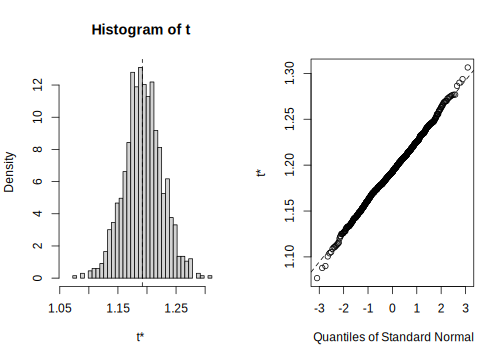
\includegraphics{Labo_BIO4558_files/figure-latex/lm-boot-2-1.pdf}

\begin{Shaded}
\begin{Highlighting}[]
\KeywordTok{plot}\NormalTok{(results, }\DataTypeTok{index=}\DecValTok{2}\NormalTok{) }\CommentTok{# log10(age)}
\end{Highlighting}
\end{Shaded}

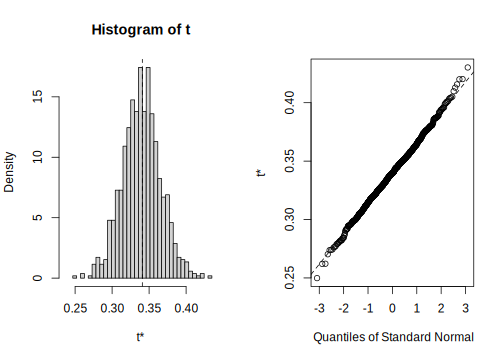
\includegraphics{Labo_BIO4558_files/figure-latex/lm-boot-2-2.pdf}

La distribution des estimés obtenus par bootstrap est assez normale dans cet exemple, avec de petites déviations dans les queuee de la distribution (là où ça compte pour les intervalles de confiance\ldots{}). On pourrait utiliser l'erreur-type des estimés bootstrap pour calculer un intervalle de confiance symétrique (moyenne +- t ET). Cependant, comme R peut facilement calculer des intervalles de confiance qui corrigent pour le biais (BCa) ou encore des intervalle empiriques à partir des distributions simulées (méthode Percentile) il peut être aussi simple de les calculer selon les 3 méthodes:

\begin{Shaded}
\begin{Highlighting}[]
\CommentTok{# interval de confiance pour l'ordonnée à l'origine}
\KeywordTok{boot.ci}\NormalTok{(results, }\DataTypeTok{type =} \StringTok{"all"}\NormalTok{, }\DataTypeTok{index =} \DecValTok{1}\NormalTok{)}
\end{Highlighting}
\end{Shaded}

\begin{verbatim}
## Warning in boot.ci(results, type = "all", index = 1): bootstrap variances needed
## for studentized intervals
\end{verbatim}

\begin{verbatim}
## BOOTSTRAP CONFIDENCE INTERVAL CALCULATIONS
## Based on 1000 bootstrap replicates
## 
## CALL : 
## boot.ci(boot.out = results, type = "all", index = 1)
## 
## Intervals : 
## Level      Normal              Basic         
## 95%   ( 1.124,  1.256 )   ( 1.124,  1.259 )  
## 
## Level     Percentile            BCa          
## 95%   ( 1.125,  1.260 )   ( 1.115,  1.250 )  
## Calculations and Intervals on Original Scale
## Some BCa intervals may be unstable
\end{verbatim}

\begin{Shaded}
\begin{Highlighting}[]
\CommentTok{#intervalle de confiance pour la pente}
\KeywordTok{boot.ci}\NormalTok{(results, }\DataTypeTok{type =} \StringTok{"all"}\NormalTok{, }\DataTypeTok{index =} \DecValTok{2}\NormalTok{)}
\end{Highlighting}
\end{Shaded}

\begin{verbatim}
## Warning in boot.ci(results, type = "all", index = 2): bootstrap variances needed
## for studentized intervals
\end{verbatim}

\begin{verbatim}
## BOOTSTRAP CONFIDENCE INTERVAL CALCULATIONS
## Based on 1000 bootstrap replicates
## 
## CALL : 
## boot.ci(boot.out = results, type = "all", index = 2)
## 
## Intervals : 
## Level      Normal              Basic         
## 95%   ( 0.2897,  0.3948 )   ( 0.2908,  0.3938 )  
## 
## Level     Percentile            BCa          
## 95%   ( 0.2879,  0.3909 )   ( 0.2953,  0.4051 )  
## Calculations and Intervals on Original Scale
\end{verbatim}

Ici, les 4 types d'intervalles de confiance que R a calculé sont essentiellement semblables. Si les données avaient violé plus sévèrement les conditions d'application de la régression (normalité, homoscedasticité), alors les différentes méthodes (Normal, Basic, Percentile, et BCa) auraient divergé un peu plus. Lequel choisir alors? BCa est celui qui est préféré de la majorité des praticiens, présentement.

\hypertarget{comparaison-de-deux-uxe9chantillons}{%
\chapter{Comparaison de deux échantillons}\label{comparaison-de-deux-uxe9chantillons}}

Après avoir complété cet exercice de laboratoire, vous devriez pouvoir:

\begin{itemize}
\tightlist
\item
  Utiliser R pour examiner visuellement vos données
\item
  Utiliser R pour comparer les moyennes de deux échantillons tirés de populations normales
\item
  Utiliser R pour comparer les moyennes de deux échantillons tirés de populations qui ne sont pas normales
\item
  Utiliser R pour comparer les moyennes de deux échantillons appariés.
\end{itemize}

\hypertarget{set-t}{%
\section{Paquets et données requises pour le labo}\label{set-t}}

Ce laboratoire nécessite:

\begin{itemize}
\tightlist
\item
  les paquets R:

  \begin{itemize}
  \tightlist
  \item
    car
  \item
    lmtest
  \item
    boot
  \item
    lmPerm
  \end{itemize}
\item
  les fichiers de données

  \begin{itemize}
  \tightlist
  \item
    sturgeon.csv
  \item
    skulldat.csv
  \end{itemize}
\end{itemize}

\hypertarget{examen-visuel-des-donnuxe9es}{%
\section{Examen visuel des données}\label{examen-visuel-des-donnuxe9es}}

Une des premières étapes dans toute analyse de données est l'examen visuel des données par des graphiques et statistiques sommaires pour détecter les distributions sous-jacentes, les valeurs extrêmes et les tendances dans vos données. Cela commence souvent avec des graphiques de vos données (histogrammes, diagrammes de probabilité, Box plots, etc.) qui vous permettent d'évaluer si vos données sont normales, si elles sont corrélées les unes aux autres, ou s'il y a des valeurs suspectes dans le fichier.

Supposons que l'on veuille comparer la distribution en taille des esturgeons de The Pas et Cumberland House. La variable \texttt{fklngth} dans le fichier \texttt{sturgeon.csv} représente la longueur (en cm) à la fourche de chaque poisson mesurée de l'extrémité de la tête à la base de la fourche de la nageoire caudale. Pour commencer, examinons si cette variable est normalement distribuée. On ne va pas tester pour la normalité à ce stade-ci; la présomption de normalité dans les analyses paramétriques s'applique aux résidus et non aux données brutes. Cependant, si les données brutes ne sont pas normales, vous avez d'habitude une très bonne raison de soupçonner que les résidus vont aussi ne pas avoir une distribution normale.

Une excellente façon de comparer visuellement une distribution à la distribution normale est de superposer un histogramme des données observées à une courbe normale. Pour ce faire, il faut procéder en deux étapes :

\begin{enumerate}
\def\labelenumi{\arabic{enumi}.}
\tightlist
\item
  indiquer à R que nous voulons créer un histogramme superposé à une courbe normale
\item
  spécifier qu'on veut que les graphiques soient faits pour les deux sites
\end{enumerate}

\begin{itemize}
\tightlist
\item
  En utilisant les données du fichier \texttt{sturgeon.csv}, générez les histogrammes et les approximations des distributions normales ajustées aux données de \texttt{fklngth} à \texttt{The\ Pas} et \texttt{Cumberland\ House}.
\end{itemize}

\begin{Shaded}
\begin{Highlighting}[]
\CommentTok{# use "sturgeon" dataframe to make plot called mygraph}
\CommentTok{# and define x axis as representing fklngth}
\NormalTok{mygraph <-}\StringTok{ }\KeywordTok{ggplot}\NormalTok{(}
  \DataTypeTok{data =}\NormalTok{ sturgeon,}
  \KeywordTok{aes}\NormalTok{(}\DataTypeTok{x =}\NormalTok{ fklngth)) }\OperatorTok{+}
\StringTok{  }\KeywordTok{xlab}\NormalTok{(}\StringTok{"Fork length (cm)"}\NormalTok{)}
\CommentTok{# add data to the mygraph ggplot}
\NormalTok{mygraph <-}\StringTok{ }\NormalTok{mygraph }\OperatorTok{+}
\StringTok{  }\KeywordTok{geom_density}\NormalTok{() }\OperatorTok{+}\StringTok{ }\CommentTok{# add data density smooth}
\StringTok{  }\KeywordTok{geom_rug}\NormalTok{() }\OperatorTok{+}\StringTok{ }\CommentTok{# add rug (bars at the bottom of the plot)}
\StringTok{  }\KeywordTok{geom_histogram}\NormalTok{( }\CommentTok{# add black semitransparent histogram}
    \KeywordTok{aes}\NormalTok{(}\DataTypeTok{y =}\NormalTok{ ..density..), }\DataTypeTok{color =} \StringTok{"black"}\NormalTok{, }\DataTypeTok{alpha =} \FloatTok{0.3}\NormalTok{) }\OperatorTok{+}
\StringTok{  }\CommentTok{# add normal curve in red, with mean and sd from fklength}
\StringTok{  }\KeywordTok{stat_function}\NormalTok{(}\DataTypeTok{fun =}\NormalTok{ dnorm,}
    \DataTypeTok{args =} \KeywordTok{list}\NormalTok{(}
      \DataTypeTok{mean =} \KeywordTok{mean}\NormalTok{(sturgeon}\OperatorTok{$}\NormalTok{fklngth),}
      \DataTypeTok{sd =} \KeywordTok{sd}\NormalTok{(sturgeon}\OperatorTok{$}\NormalTok{fklngth)}
\NormalTok{    ),}
    \DataTypeTok{color =} \StringTok{"red"}\NormalTok{)}
\CommentTok{#display graph, by location}
\NormalTok{mygraph}\OperatorTok{+}\KeywordTok{facet_grid}\NormalTok{(.}\OperatorTok{~}\NormalTok{location)}
\end{Highlighting}
\end{Shaded}

\begin{figure}
\centering
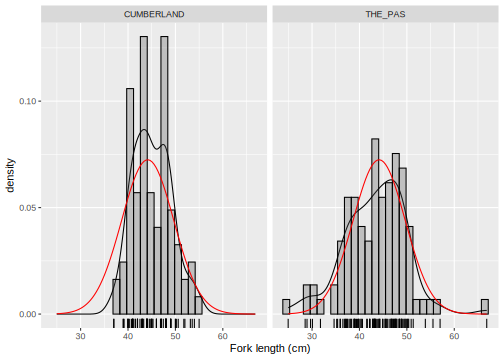
\includegraphics{Labo_BIO4558_files/figure-latex/t-1-1.pdf}
\caption{\label{fig:t-1}Distribution de la longueur des esturgeons}
\end{figure}

Examinez ce graphique et essayez de déterminer si ces deux échantillons sont normalement distribués. À mon avis, cette variable est approximativement normalement distribuée dans les deux échantillons. Puisque ce qui nous intéresse est de comparer la taille des poissons de deux sites différents, c'est probablement une bonne idée de créer un graphique qui compare les deux groupes de données. Un Box plot convient très bien pour cette tâche.

\begin{itemize}
\tightlist
\item
  Tracez un boxplot de \texttt{fklngth} groupé par \texttt{location}. Que concluez-vous quant à la différence entre les deux sites?
\end{itemize}

\begin{Shaded}
\begin{Highlighting}[]
\KeywordTok{ggplot}\NormalTok{(}\DataTypeTok{data=}\NormalTok{sturgeon, }\KeywordTok{aes}\NormalTok{(}\DataTypeTok{x=}\NormalTok{location,}
\DataTypeTok{y=}\NormalTok{fklngth))}\OperatorTok{+}\KeywordTok{geom_boxplot}\NormalTok{(}\DataTypeTok{notch=}\OtherTok{TRUE}\NormalTok{)}
\end{Highlighting}
\end{Shaded}

\begin{figure}
\centering
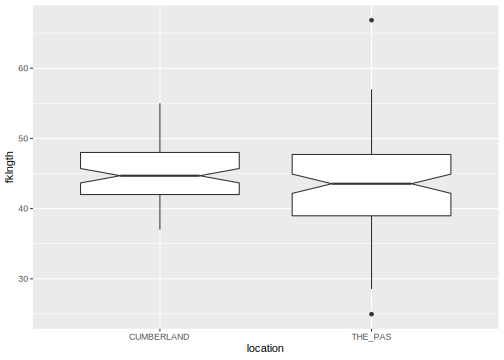
\includegraphics{Labo_BIO4558_files/figure-latex/t-2-1.pdf}
\caption{\label{fig:t-2}Boxplot de la longueur des esturgeons}
\end{figure}

Il n'y a pas de grande différence de taille entre les deux sites, mais la taille des poissons à The Pas est plus variable ayant une plus large étendue de taille et des valeurs extrêmes (définies par les valeurs qui sont \textgreater{} 1.5*l'étendue interquartile) à chaque bout de la distribution.

\hypertarget{comparer-les-moyennes-de-deux-uxe9chantillons-induxe9pendants}{%
\section{Comparer les moyennes de deux échantillons indépendants}\label{comparer-les-moyennes-de-deux-uxe9chantillons-induxe9pendants}}

Éprouvez l'hypothèse nulle d'égalité de la longueur à la fourche à The Pas et Cumberland House de 3 manières différentes:

\begin{enumerate}
\def\labelenumi{\arabic{enumi}.}
\tightlist
\item
  paramétriques supposant des variances égales
\item
  paramétriques supposant des variances différentes
\item
  non-paramétriques
\end{enumerate}

Que concluez-vous?

\begin{Shaded}
\begin{Highlighting}[]
\CommentTok{# t-test assuming equal variances}
 \KeywordTok{t.test}\NormalTok{(}
\NormalTok{   fklngth}\OperatorTok{~}\NormalTok{location, }\DataTypeTok{data =}\NormalTok{ sturgeon,}
   \DataTypeTok{alternative =}\StringTok{'two.sided'}\NormalTok{,}
   \DataTypeTok{var.equal =} \OtherTok{TRUE}\NormalTok{)}
\end{Highlighting}
\end{Shaded}

\begin{verbatim}
## 
## 	Two Sample t-test
## 
## data:  fklngth by location
## t = 2.1359, df = 184, p-value = 0.03401
## alternative hypothesis: true difference in means is not equal to 0
## 95 percent confidence interval:
##  0.1308307 3.2982615
## sample estimates:
## mean in group CUMBERLAND    mean in group THE_PAS 
##                 45.08439                 43.36984
\end{verbatim}

\begin{Shaded}
\begin{Highlighting}[]
\CommentTok{# t-test assuming unequal variances}
 \KeywordTok{t.test}\NormalTok{(}
\NormalTok{   fklngth }\OperatorTok{~}\StringTok{ }\NormalTok{location, }\DataTypeTok{data =}\NormalTok{ sturgeon,}
   \DataTypeTok{alternative =}\StringTok{'two.sided'}\NormalTok{,}
   \DataTypeTok{var.equal =} \OtherTok{FALSE}\NormalTok{)}
\end{Highlighting}
\end{Shaded}

\begin{verbatim}
## 
## 	Welch Two Sample t-test
## 
## data:  fklngth by location
## t = 2.2201, df = 169.8, p-value = 0.02774
## alternative hypothesis: true difference in means is not equal to 0
## 95 percent confidence interval:
##  0.1900117 3.2390804
## sample estimates:
## mean in group CUMBERLAND    mean in group THE_PAS 
##                 45.08439                 43.36984
\end{verbatim}

\begin{Shaded}
\begin{Highlighting}[]
\CommentTok{# test non paramétrique}
 \KeywordTok{wilcox.test}\NormalTok{(}
\NormalTok{   fklngth }\OperatorTok{~}\StringTok{ }\NormalTok{location, }\DataTypeTok{data =}\NormalTok{ sturgeon,}
   \DataTypeTok{alternative =}\StringTok{'two.sided'}\NormalTok{)}
\end{Highlighting}
\end{Shaded}

\begin{verbatim}
## 
## 	Wilcoxon rank sum test with continuity correction
## 
## data:  fklngth by location
## W = 4973, p-value = 0.06296
## alternative hypothesis: true location shift is not equal to 0
\end{verbatim}

En se fiant au test de t, on rejette donc l'hypothèse nulle. Il y a une différence significative entre les deux moyennes des longueurs à la fourche.

Notez que si l'on se fie au test de \emph{Wilcoxon}, il faut accepter l'hypothèse nulle. Les deux tests mènent donc à des conclusions contradictoires. La différence significative obtenue par le test de t peut provenir en partie d'une violation des conditions d'application du test (normalité et homoscédasticité). D'un autre côté, l'absence de différence significative selon le test de Wilcoxon pourrait être due au fait que, pour un effectif donné, la puissance du test non paramétrique est inférieure à celle du test paramétrique correspondant. Compte tenu 1) des valeurs de p obtenues pour les deux tests, et 2) le fait que pour des grands échantillons (des effectifs de 84 et 101 sont considérés grands) le test de t est considéré robuste, il est raisonnable de rejeter l'hypothèse nulle.

Avant d'accepter les résultats du test de t et de rejeter l'hypothèse nulle qu'il n'y a pas de différences de taille entre les deux sites, il est important de déterminer si les données remplissent les conditions de normalité des résidus et d'égalité des variances. L'examen préliminaire suggérait que les données sont à peu près normales mais qu'il y avait peut-être des problèmes avec les variances (puisque l'étendue des données pour The Pas était beaucoup plus grande que celle pour Cumberland). On peut examiner ces conditions d'application plus en détail en examinant les résidus d'un modèle linéaire et en utilisant les graphiques diagnostiques:

\begin{Shaded}
\begin{Highlighting}[]
\NormalTok{m1 <-}\StringTok{ }\KeywordTok{lm}\NormalTok{(fklngth }\OperatorTok{~}\StringTok{ }\NormalTok{location, }\DataTypeTok{data=}\NormalTok{sturgeon)}
\KeywordTok{par}\NormalTok{(}\DataTypeTok{mfrow =} \KeywordTok{c}\NormalTok{(}\DecValTok{2}\NormalTok{, }\DecValTok{2}\NormalTok{))}
\KeywordTok{plot}\NormalTok{(m1)}
\end{Highlighting}
\end{Shaded}

\begin{figure}
\centering
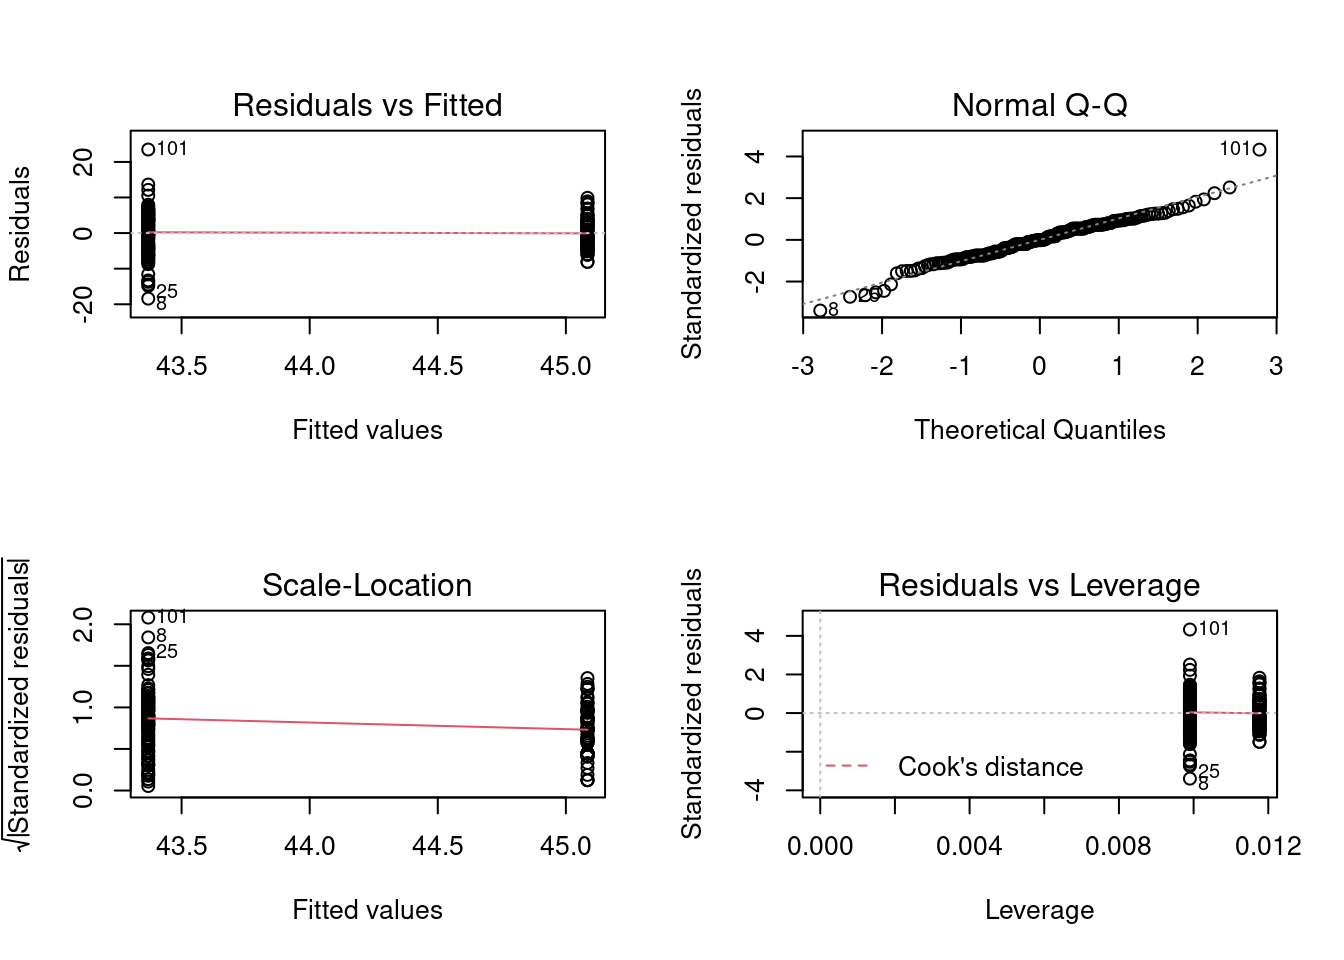
\includegraphics{Labo_BIO4558_files/figure-latex/t-6-1.pdf}
\caption{\label{fig:t-6}Condition d'application du modèle linéaire}
\end{figure}

Le premier graphique ci-dessus montre comment les résidus se distribuent autour des valeurs prédites (les moyennes) pour chaque site et permette de juger si il semble y avoir un problème de normalité ou d'homoscédasticité. Si les variances étaient égales dans les deux sites, l'étendue verticale des résidus tendrait à être la même. Sur le graphique, on voit que l'étendue des résidus est plus grande à gauche (le site où la taille moyenne est la plus faible), ce qui suggère un possible problème d'homogénéité des variances. On peut tester cela plus formellement en comparant la moyenne de la valeur absolue des résidus.(on y reviendra; c'est le test de Levene).

Le second graphique est un graphique de probabilité (graphique Q-Q) des résidus. Comme ici, les points tombent près de la diagonale, il ne semble pas y avoir de problème important avec la normalité. On peut faire un test formel de la condition de normalité par le test de Shapiro- Wilk:

\begin{Shaded}
\begin{Highlighting}[]
\KeywordTok{shapiro.test}\NormalTok{(}\KeywordTok{residuals}\NormalTok{(m1))}
\end{Highlighting}
\end{Shaded}

\begin{verbatim}
## 
## 	Shapiro-Wilk normality test
## 
## data:  residuals(m1)
## W = 0.97469, p-value = 0.001857
\end{verbatim}

Hummm. Ce test indique que les résidus ne sont pas normaux, ce qui contredit notre évaluation visuelle. Cependant, puisque (a) la distribution des résidus ne s'éloigne pas beaucoup de la normalité et (b) le nombre d'observations à chaque site est raisonnablement grand (i.e.~\textgreater{}30), on n'a pas à être trop inquiet quant à l'impact de cette violation de normalité sur la fiabilité du test.

Qu'en est-il de l'égalité des variances?

\begin{Shaded}
\begin{Highlighting}[]
 \KeywordTok{leveneTest}\NormalTok{(m1)}
\end{Highlighting}
\end{Shaded}

\begin{verbatim}
## Warning in leveneTest.default(y = y, group = group, ...): group coerced to
## factor.
\end{verbatim}

\begin{verbatim}
## Levene's Test for Homogeneity of Variance (center = median)
##        Df F value    Pr(>F)    
## group   1  11.514 0.0008456 ***
##       184                      
## ---
## Signif. codes:  0 '***' 0.001 '**' 0.01 '*' 0.05 '.' 0.1 ' ' 1
\end{verbatim}

\begin{Shaded}
\begin{Highlighting}[]
\KeywordTok{bptest}\NormalTok{(m1)}
\end{Highlighting}
\end{Shaded}

\begin{verbatim}
## 
## 	studentized Breusch-Pagan test
## 
## data:  m1
## BP = 8.8015, df = 1, p-value = 0.00301
\end{verbatim}

Les résultats qui précédents proviennent de 3 des tests disponibles en R (dans les package car et lmtest) qui éprouvent l'hypothèse de l'égalité des variances dans des tests de t ou des modèles linéaires ayant uniquement des variables indépendantes discontinues ou catégoriques. Il est redondant de faire les 2 tests. Si ils sont présentés ici, c'est que ces 2 tests sont usuels et qu'il n'y a pas consensus quant au meilleur des deux. Le test de Levene est le plus connu et utilisé. Il compare la moyenne des valeurs absolues des résidus dans les deux groupes. Le test Breusch-Pagan a l'avantage d'être applicable à une plus large gamme de modèles linéaires (il peut être utilisé également avec des variables indépendantes continues, comme en régression). Ici, les deux tests mènent à la même conclusion: la variance diffère entre les deux sites.

Sur la base de ces résultats, on peut conclure qu'il y a évidence (mais faible) pour rejeter l'hypothèse nulle qu'il n'y a pas de différence dans la taille de poissons entre les deux sites. On a utilisé une modification du test de t pour tenir compte du fait que les variances ne sont pas égales et nous sommes satisfaits que la condition de normalité des résidus a été remplie. Alors, fklngth à Cumberland est plus grande que fklngth à The Pas.

\hypertarget{bootstrap-et-tests-de-permutation-pour-comparer-deux-moyennes}{%
\section{Bootstrap et tests de permutation pour comparer deux moyennes}\label{bootstrap-et-tests-de-permutation-pour-comparer-deux-moyennes}}

\hypertarget{bootstrap}{%
\subsection{Bootstrap}\label{bootstrap}}

Le bootstrap et les tests de permutation peuvent être utilisés pour comparer les moyennes (ou d'autres statistiques). Le principe général est simple et peut être effectué de diverses façons. Ici j'utilise certains des outils disponibles et le fait qu'une comparaison de moyenne peut être représentée par un modèle linéaire. On pourra utiliser un programme similaire plus tard quand on ajustera des modèles plus complexes.

\texttt{library(boot)}

La première section sert à définir une fonction (ici appelée bs) qui extraie les coefficients d'un modèle ajusté :

\begin{Shaded}
\begin{Highlighting}[]
\CommentTok{# function to obtain model coefficients for each iteration}
\NormalTok{bs <-}\StringTok{ }\ControlFlowTok{function}\NormalTok{(formula, data, indices) \{}
\NormalTok{  d <-}\StringTok{ }\NormalTok{data[indices, ]}
\NormalTok{  fit <-}\StringTok{ }\KeywordTok{lm}\NormalTok{(formula, }\DataTypeTok{data =}\NormalTok{ d)}
  \KeywordTok{return}\NormalTok{(}\KeywordTok{coef}\NormalTok{(fit))}
\NormalTok{\}}
\end{Highlighting}
\end{Shaded}

La deuxième section avec la commande boot() fait le gros du travail: on prend les données dans sturgeon, on les bootstrap \(R = 1000\) fois, et chaque fois on ajuste le modèle \texttt{fklngth} vs \texttt{location} et on garde les valeurs calculées par la fonction \texttt{bs}.

\begin{Shaded}
\begin{Highlighting}[]
\CommentTok{# bootstrapping with 1000 replications}
\NormalTok{results <-}\StringTok{ }\KeywordTok{boot}\NormalTok{(}\DataTypeTok{data =}\NormalTok{ sturgeon, }\DataTypeTok{statistic =}\NormalTok{ bs, }\DataTypeTok{R =} \DecValTok{1000}\NormalTok{,}
\DataTypeTok{formula =}\NormalTok{ fklngth }\OperatorTok{~}\StringTok{ }\NormalTok{location)}
\CommentTok{# view results}
\NormalTok{results}
\end{Highlighting}
\end{Shaded}

\begin{verbatim}
## 
## ORDINARY NONPARAMETRIC BOOTSTRAP
## 
## 
## Call:
## boot(data = sturgeon, statistic = bs, R = 1000, formula = fklngth ~ 
##     location)
## 
## 
## Bootstrap Statistics :
##      original      bias    std. error
## t1* 45.084391 -0.01071599   0.4219215
## t2* -1.714546  0.03221483   0.7613399
\end{verbatim}

On obtient les estimés originaux pour les deux coefficients du modèle: la moyenne pour le premier (alphabétiquement) site soit Cumberland, et la différence entre les deux moyennes à Cumberland et The Pas. C'est ce second paramètre, la différence entre les moyennes, qui nous intéresse.

\begin{Shaded}
\begin{Highlighting}[]
\KeywordTok{plot}\NormalTok{(results, }\DataTypeTok{index =} \DecValTok{2}\NormalTok{)}
\end{Highlighting}
\end{Shaded}

\begin{figure}
\centering
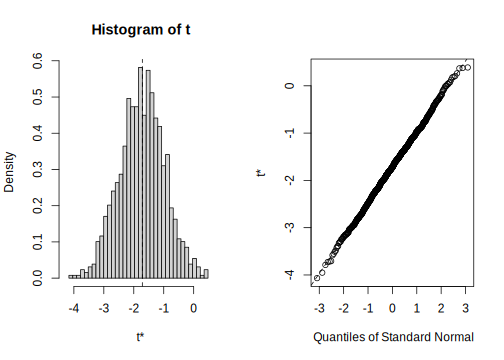
\includegraphics{Labo_BIO4558_files/figure-latex/tb-3-1.pdf}
\caption{\label{fig:tb-3}Normalité des estimés de la différence des moyennes par bootstrap}
\end{figure}

\begin{Shaded}
\begin{Highlighting}[]
\CommentTok{# get 95% confidence intervals}
\KeywordTok{boot.ci}\NormalTok{(results, }\DataTypeTok{type =} \StringTok{"bca"}\NormalTok{, }\DataTypeTok{index =} \DecValTok{2}\NormalTok{)}
\end{Highlighting}
\end{Shaded}

\begin{verbatim}
## BOOTSTRAP CONFIDENCE INTERVAL CALCULATIONS
## Based on 1000 bootstrap replicates
## 
## CALL : 
## boot.ci(boot.out = results, type = "bca", index = 2)
## 
## Intervals : 
## Level       BCa          
## 95%   (-3.289, -0.255 )  
## Calculations and Intervals on Original Scale
\end{verbatim}

Comme l'intervalle de confiance n'inclue pas 0, on conclue que les moyennes ne sont pas les mêmes.

\hypertarget{permutation}{%
\subsection{Permutation}\label{permutation}}

Les tests de permutation pour les modèles linéaires peuvent être effectués à l'aide du package \texttt{lmPerm}:

\begin{Shaded}
\begin{Highlighting}[]
\NormalTok{m1Perm <-}\StringTok{ }\KeywordTok{lmp}\NormalTok{(}
\NormalTok{  fklngth }\OperatorTok{~}\StringTok{ }\NormalTok{location, }\DataTypeTok{data =}\NormalTok{ sturgeon,}
  \DataTypeTok{perm =} \StringTok{"Prob"}\NormalTok{)}
\end{Highlighting}
\end{Shaded}

\begin{verbatim}
## [1] "Settings:  unique SS "
\end{verbatim}

La fonction \texttt{lmp()} fait tout le travail pour nous. Ici, cette fonction est effectuée avec l'option perm pour choisir la règle utilisée pour stopper les calculs. L'option Probs arrête les permutations quand la déviation standard estimée pour la p-valeur tombe sous un seuil déterminé. C'est l'une des nombreuses règles qui peuvent possiblement être utilisées pour ne faire les permutations que sur un sous-ensemble des permutations possibles (ce qui prendrait souvent trrrrrès longthemps).

\begin{Shaded}
\begin{Highlighting}[]
\KeywordTok{summary}\NormalTok{(m1Perm)}
\end{Highlighting}
\end{Shaded}

\begin{verbatim}
## 
## Call:
## lmp(formula = fklngth ~ location, data = sturgeon, perm = "Prob")
## 
## Residuals:
##       Min        1Q    Median        3Q       Max 
## -18.40921  -3.75370  -0.08439   3.76598  23.48055 
## 
## Coefficients:
##           Estimate Iter Pr(Prob)  
## location1   0.8573 1966   0.0488 *
## ---
## Signif. codes:  0 '***' 0.001 '**' 0.01 '*' 0.05 '.' 0.1 ' ' 1
## 
## Residual standard error: 5.454 on 184 degrees of freedom
## Multiple R-Squared: 0.02419,	Adjusted R-squared: 0.01889 
## F-statistic: 4.562 on 1 and 184 DF,  p-value: 0.03401
\end{verbatim}

\begin{enumerate}
\def\labelenumi{\arabic{enumi}.}
\tightlist
\item
  Ici, la règle a limité à 1117 permutations le calcul. Notez que ce nombre va varier à chaque fois que vous tournerez cet petit bout de code. Ce sont des résultats obtenus par permutations aléatoires, donc vous devez vous attendre à de la variabilité. .
\item
  La p-valeur estimée pour H0 est 0.0824. La différence observée pour fklngth between entre les deux sites était plus grande que les valeurs permutées environ (1-0.0824=presque 92\%) des 1117 permutations. Notez que 1117 permutations ce n'est pas un si grand nombre de permutations que ça, et donc les faibles valeurs de p ne sont pas très précises. Si vous voulez des valeurs précises de p, vous devrez faire plus de permutations.. Vous pouvez ajuster 2 paramètres: maxIter, le nombre maximal de permutations (défaut 5000) et Ca, le seuil de précision désiré qui arrête les permutations quand l'erreur- type de p est plus petite que Ca*p (défaut=0.1)
\item
  Le reste est la sortie standard pour un modèle ajusté à des
  données, avec le test paramétrique. Ici, la p-valeur, présumant que toutes les conditions d'application sont remplies, est 0.34.
\end{enumerate}

\hypertarget{comparer-les-moyennes-de-deux-uxe9chantillons-appariuxe9s}{%
\section{Comparer les moyennes de deux échantillons appariés}\label{comparer-les-moyennes-de-deux-uxe9chantillons-appariuxe9s}}

Dans certaines expériences les mêmes individus sont mesurés deux fois, par exemple avant et après un traitement ou encore à deux moments au cours de leur développement. Les mesures obtenues lors de ces deux événements ne sont pas indépendantes, et des comparaisons de ces mesures appariées doivent être faites.

Le fichier \texttt{skulldat.csv} contient des mesures de la partie inférieure du visage de jeunes filles d'Amérique du Nord prises à 5 ans, puis à 6 ans (données de Newman and Meredith, 1956).

\begin{itemize}
\tightlist
\item
  Pour débuter, éprouvons l'hypothèse que la largeur de la figure est la même à 5 ans et à 6 ans en assumant que les mesures viennent d'échantillons indépendants.
\end{itemize}

\begin{Shaded}
\begin{Highlighting}[]
\NormalTok{skull <-}\StringTok{ }\KeywordTok{read.csv}\NormalTok{(}\StringTok{"data/skulldat.csv"}\NormalTok{)}
\KeywordTok{t.test}\NormalTok{(width}\OperatorTok{~}\NormalTok{age, }\DataTypeTok{data =}\NormalTok{ skull,}
  \DataTypeTok{alternative=}\StringTok{'two.sided'}\NormalTok{,}
  \DataTypeTok{paired =} \OtherTok{FALSE}\NormalTok{)}
\end{Highlighting}
\end{Shaded}

\begin{verbatim}
## 
## 	Welch Two Sample t-test
## 
## data:  width by age
## t = -1.7812, df = 27.93, p-value = 0.08576
## alternative hypothesis: true difference in means is not equal to 0
## 95 percent confidence interval:
##  -0.43002624  0.03002624
## sample estimates:
## mean in group 5 mean in group 6 
##        7.461333        7.661333
\end{verbatim}

Maintenant, effectuons le test apparié qui est approprié: Que conclure? Com- ment les résultats diffèrent-ils de la première analyse? Pourquoi?

\begin{Shaded}
\begin{Highlighting}[]
\KeywordTok{t.test}\NormalTok{(width}\OperatorTok{~}\NormalTok{age, }\DataTypeTok{data =}\NormalTok{ skull,}
  \DataTypeTok{alternative=}\StringTok{'two.sided'}\NormalTok{,}
  \DataTypeTok{paired =} \OtherTok{TRUE}\NormalTok{)}
\end{Highlighting}
\end{Shaded}

\begin{verbatim}
## 
## 	Paired t-test
## 
## data:  width by age
## t = -19.72, df = 14, p-value = 1.301e-11
## alternative hypothesis: true difference in means is not equal to 0
## 95 percent confidence interval:
##  -0.2217521 -0.1782479
## sample estimates:
## mean of the differences 
##                    -0.2
\end{verbatim}

La première analyse a comme supposition que les deux échantillons de filles de 5 et 6 ans sont indépendants, alors que la deuxième analyse a comme supposition que la même fille a été mesurée deux fois, une fois à 5 ans, et la deuxième fois à 6 ans.

Notez que, dans le premier cas, on accepte l'hypothèse nulle, mais que le test apparié rejette l'hypothèse nulle. Donc, le test qui est approprié (le test apparié) indique un effet très significatif de l'âge, mais le test inapproprié suggère que l'âge n'importe pas. C'est parce qu'il y a une très forte corrélation entre la largeur du visage à 5 et 6 ans:

\begin{Shaded}
\begin{Highlighting}[]
\NormalTok{graphskull <-}\StringTok{ }\KeywordTok{ggplot}\NormalTok{(}\DataTypeTok{data =}\NormalTok{ skull, }\KeywordTok{aes}\NormalTok{(}\DataTypeTok{x =}\NormalTok{ width5, }\DataTypeTok{y =}\NormalTok{ width6)) }\OperatorTok{+}
\StringTok{  }\KeywordTok{geom_point}\NormalTok{() }\OperatorTok{+}
\StringTok{  }\KeywordTok{labs}\NormalTok{(}\DataTypeTok{x =} \StringTok{"Skull width at age 5"}\NormalTok{, }\DataTypeTok{y =} \StringTok{"Skull width at age 6"}\NormalTok{) }\OperatorTok{+}
\StringTok{  }\KeywordTok{geom_smooth}\NormalTok{() }\OperatorTok{+}
\StringTok{  }\KeywordTok{scale_fill_continuous}\NormalTok{(}\DataTypeTok{low=}\StringTok{"lavenderblush"}\NormalTok{, }\DataTypeTok{high=}\StringTok{"red"}\NormalTok{)}
\NormalTok{graphskull}
\end{Highlighting}
\end{Shaded}

\begin{verbatim}
## `geom_smooth()` using method = 'loess' and formula 'y ~ x'
\end{verbatim}

\begin{figure}
\centering
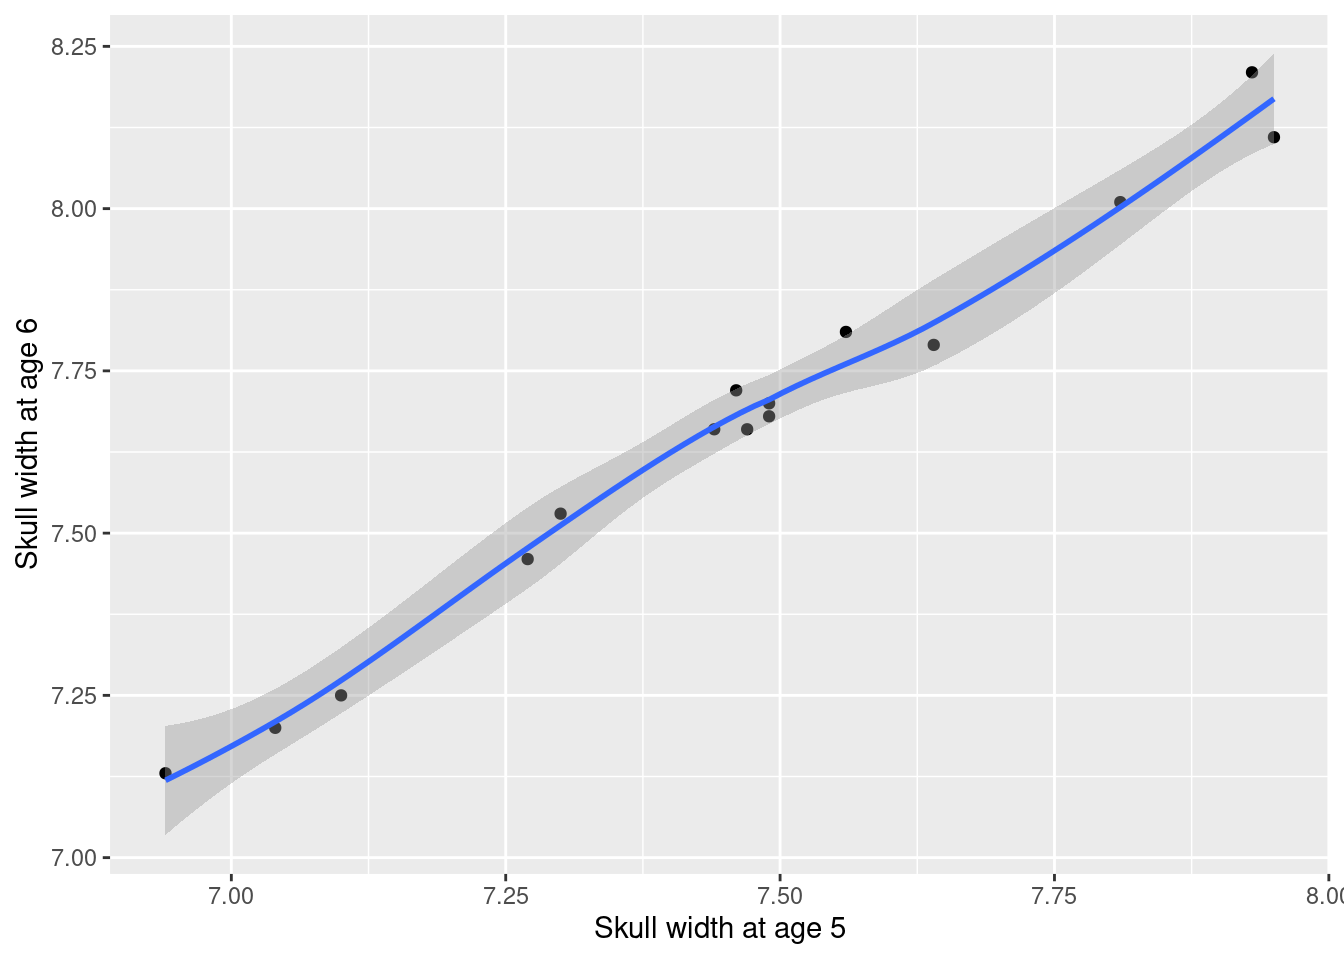
\includegraphics{Labo_BIO4558_files/figure-latex/tpaired-3-1.pdf}
\caption{\label{fig:tpaired-3}Relation entre la taille de la tête à 5 et 6 ans}
\end{figure}

Avec \emph{r} = NA. En présence d'une si forte corrélation, l'erreur-type de la différence appariée de largeur du visage entre 5 et 6 ans est beaucoup plus petit que l'erreur-type de la différence entre la largeur moyenne à 5 ans et la largeur moyenne à 6 ans. Par conséquent, la statistique t associée est beaucoup plus élevée pour le test apparié, la puissance du test est plus grande, et la valeur de p plus petite.

\begin{itemize}
\tightlist
\item
  Répétez l'analyse en utilisant l'alternative nonparamétrique, le test Wil-coxon signed-rank. ( Que concluez-vous?
\end{itemize}

\begin{Shaded}
\begin{Highlighting}[]
\KeywordTok{wilcox.test}\NormalTok{(width}\OperatorTok{~}\NormalTok{age, }\DataTypeTok{data =}\NormalTok{ skull,}
  \DataTypeTok{alternative=}\StringTok{'two.sided'}\NormalTok{,}
  \DataTypeTok{paired =} \OtherTok{TRUE}\NormalTok{)}
\end{Highlighting}
\end{Shaded}

\begin{verbatim}
## Warning in wilcox.test.default(x = c(7.33, 7.49, 7.27, 7.93, 7.56, 7.81, :
## cannot compute exact p-value with ties
\end{verbatim}

\begin{verbatim}
## 
## 	Wilcoxon signed rank test with continuity correction
## 
## data:  width by age
## V = 0, p-value = 0.0007193
## alternative hypothesis: true location shift is not equal to 0
\end{verbatim}

Donc on tire la même conclusion qu'avec le test de t apparié et conclue qu'il y a des différences significatives entre la taille des crânes de filles âgées de 5 et 6 ans (quelle surprise!).

Mais, attendez une minute! On a utilisé des tests bilatéraux ici mais, compte tenu de s connaissances sur la croissance des enfants, une hypothèse unilatérale serait préférable. Ceci peut être accommodé en modifiant l'option ``alternative''. On utilise l'hypothèse alternative pour décider entre ``less'' ou ``greater''. Ici on s'attends que si il y a une différence, width5 va être inférieur à width6, donc on utiliserait ``less''.

\begin{Shaded}
\begin{Highlighting}[]
\KeywordTok{t.test}\NormalTok{(width}\OperatorTok{~}\NormalTok{age, }\DataTypeTok{data =}\NormalTok{ skull,}
  \DataTypeTok{alternative=}\StringTok{'less'}\NormalTok{,}
  \DataTypeTok{paired =} \OtherTok{TRUE}\NormalTok{)}
\end{Highlighting}
\end{Shaded}

\begin{verbatim}
## 
## 	Paired t-test
## 
## data:  width by age
## t = -19.72, df = 14, p-value = 6.507e-12
## alternative hypothesis: true difference in means is less than 0
## 95 percent confidence interval:
##        -Inf -0.1821371
## sample estimates:
## mean of the differences 
##                    -0.2
\end{verbatim}

\begin{Shaded}
\begin{Highlighting}[]
\KeywordTok{wilcox.test}\NormalTok{(width}\OperatorTok{~}\NormalTok{age, }\DataTypeTok{data =}\NormalTok{ skull,}
  \DataTypeTok{alternative=}\StringTok{'less'}\NormalTok{,}
  \DataTypeTok{paired =} \OtherTok{TRUE}\NormalTok{)}
\end{Highlighting}
\end{Shaded}

\begin{verbatim}
## Warning in wilcox.test.default(x = c(7.33, 7.49, 7.27, 7.93, 7.56, 7.81, :
## cannot compute exact p-value with ties
\end{verbatim}

\begin{verbatim}
## 
## 	Wilcoxon signed rank test with continuity correction
## 
## data:  width by age
## V = 0, p-value = 0.0003597
## alternative hypothesis: true location shift is less than 0
\end{verbatim}

\hypertarget{ruxe9fuxe9rences}{%
\section{Références}\label{ruxe9fuxe9rences}}

Bumpus, H.C. (1898) The elimination of the unfit as illustrated by the introduced sparrow, Passer domesticus. Biological Lectures, Woods Hole Biology Laboratory, Woods Hole, 11 th Lecture: 209 - 226.

Newman, K.J. and H.V. Meredith. (1956) Individual growth in skele- tal bigonial diameter during the childhood period from 5 to 11 years of age. Amer. J. Anat. 99: 157 - 187.

\hypertarget{anova-uxe0-un-crituxe8re-de-classification}{%
\chapter{ANOVA à un critère de classification}\label{anova-uxe0-un-crituxe8re-de-classification}}

Après avoir complété cet exercice de laboratoire, vous devriez être capable de :

\begin{itemize}
\tightlist
\item
  Utiliser R pour effectuer une analyse de variance paramétrique à un critère de classification, suivie de comparaisons multiples * Utiliser R pour vérifier si les conditions d'application de l'ANOVA paramétrique sont remplies * Utiliser R pour faire une ANOVA à un critère de classification non-paramétrique * Utiliser R pour transformer des données de manière à mieux rem- plir les conditions d'application de l'ANOVA paramétrique.
\end{itemize}

\hypertarget{set-ano}{%
\section{Paquets et données requises pour le labo}\label{set-ano}}

Ce laboratoire nécessite:

\begin{itemize}
\tightlist
\item
  les paquets R:

  \begin{itemize}
  \tightlist
  \item
    multicomp
  \item
    car
  \end{itemize}
\item
  les fichiers de données

  \begin{itemize}
  \tightlist
  \item
    Dam10dat.csv
  \end{itemize}
\end{itemize}

\hypertarget{anova-uxe0-un-crituxe8re-de-classification-et-comparaisons-multiples}{%
\section{ANOVA à un critère de classification et comparaisons multiples}\label{anova-uxe0-un-crituxe8re-de-classification-et-comparaisons-multiples}}

L'ANOVA à un critère de classification est l'analogue du test de t pour des comparaisons de moyennes de plus de deux échantillons. Les conditions d'application du test sont essentiellement les mêmes, et lorsque appliqué à deux échantillons ce test est mathématiquement équivalent au test de t.

En 1961-1962, le barrage Grand Rapids était construit sur la rivière Saskatchewan en amont de Cumberland House. On croit que durant la construction plusieurs gros esturgeons restèrent prisonniers dans des sections peu profondes et moururent. Des inventaires de la population d'esturgeons furent faits en 1954, 1958, 1965 et 1966. Au cours de ces inventaires, la longueur à la fourche ( frklngth ) et la masse ( rndwght ) furent mesurées (pas nécessairement sur chaque poisson cependant). Ces données sont dans le fichier \texttt{Dam10dat.csv}.

\hypertarget{visualiser-les-donnuxe9es}{%
\subsection{Visualiser les données}\label{visualiser-les-donnuxe9es}}

\begin{itemize}
\tightlist
\item
  À partir des données, vous devez d'abord changer le type de donnée de la variable \texttt{year}, pour que R traite \texttt{year} comme une variable discontinue (factor) plutôt que continue.
\end{itemize}

\begin{Shaded}
\begin{Highlighting}[]
\NormalTok{Dam10dat <-}\StringTok{ }\KeywordTok{read.csv}\NormalTok{(}\StringTok{"data/Dam10dat.csv"}\NormalTok{)}
\NormalTok{Dam10dat}\OperatorTok{$}\NormalTok{year <-}\StringTok{ }\KeywordTok{as.factor}\NormalTok{(Dam10dat}\OperatorTok{$}\NormalTok{year)}
\KeywordTok{str}\NormalTok{(Dam10dat)}
\end{Highlighting}
\end{Shaded}

\begin{verbatim}
## 'data.frame':	118 obs. of  21 variables:
##  $ year    : Factor w/ 4 levels "1954","1958",..: 1 1 1 1 1 1 1 1 1 1 ...
##  $ fklngth : num  45 50 39 46 54.5 49 42.5 49 56 54 ...
##  $ totlngth: num  49 NA 43 50.5 NA 51.7 45.5 52 60.2 58.5 ...
##  $ drlngth : logi  NA NA NA NA NA NA ...
##  $ drwght  : num  16 20.5 10 17.5 19.7 21.3 9.5 23.7 31 27.3 ...
##  $ rdwght  : num  24.5 33 15.5 28.5 32.5 35.5 15.3 40.5 51.5 43 ...
##  $ sex     : int  1 1 1 2 1 2 1 1 1 1 ...
##  $ age     : int  24 33 17 31 37 44 23 34 33 47 ...
##  $ lfkl    : num  1.65 1.7 1.59 1.66 1.74 ...
##  $ ltotl   : num  1.69 NA 1.63 1.7 NA ...
##  $ ldrl    : logi  NA NA NA NA NA NA ...
##  $ ldrwght : num  1.2 1.31 1 1.24 1.29 ...
##  $ lrdwght : num  1.39 1.52 1.19 1.45 1.51 ...
##  $ lage    : num  1.38 1.52 1.23 1.49 1.57 ...
##  $ rage    : int  4 6 3 6 7 7 4 6 6 7 ...
##  $ ryear   : int  1954 1954 1954 1954 1954 1954 1954 1954 1954 1954 ...
##  $ ryear2  : int  1958 1958 1958 1958 1958 1958 1958 1958 1958 1958 ...
##  $ ryear3  : int  1966 1966 1966 1966 1966 1966 1966 1966 1966 1966 ...
##  $ location: int  1 1 1 1 1 1 1 1 1 1 ...
##  $ girth   : logi  NA NA NA NA NA NA ...
##  $ lgirth  : logi  NA NA NA NA NA NA ...
\end{verbatim}

\begin{itemize}
\tightlist
\item
  Ensuite, visualisez les données comme dans le labo pour les tests de t. Créez un histogramme avec ligne de densité, un diagramme de probabilité, et un Box plot par année. Que vous révèlent ces données?
\end{itemize}

\begin{Shaded}
\begin{Highlighting}[]
\NormalTok{mygraph <-}\StringTok{ }\KeywordTok{ggplot}\NormalTok{(Dam10dat, }\KeywordTok{aes}\NormalTok{(}\DataTypeTok{x =}\NormalTok{ fklngth)) }\OperatorTok{+}
\StringTok{  }\KeywordTok{labs}\NormalTok{ (}\DataTypeTok{x =} \StringTok{"Fork length (cm)"}\NormalTok{) }\OperatorTok{+}
\StringTok{  }\KeywordTok{geom_density}\NormalTok{() }\OperatorTok{+}
\StringTok{  }\KeywordTok{geom_rug}\NormalTok{() }\OperatorTok{+}
\StringTok{  }\KeywordTok{geom_histogram}\NormalTok{(}\KeywordTok{aes}\NormalTok{(}\DataTypeTok{y =}\NormalTok{ ..density..),}
    \DataTypeTok{color =} \StringTok{"black"}\NormalTok{,}
    \DataTypeTok{alpha =} \FloatTok{0.3}\NormalTok{) }\OperatorTok{+}
\StringTok{  }\KeywordTok{stat_function}\NormalTok{(}\DataTypeTok{fun =}\NormalTok{ dnorm,}
    \DataTypeTok{args =} \KeywordTok{list}\NormalTok{(}
      \DataTypeTok{mean =} \KeywordTok{mean}\NormalTok{(Dam10dat}\OperatorTok{$}\NormalTok{fklngth),}
      \DataTypeTok{sd =} \KeywordTok{sd}\NormalTok{(Dam10dat}\OperatorTok{$}\NormalTok{fklngth)),}
    \DataTypeTok{color =} \StringTok{"red"}\NormalTok{)}

\CommentTok{#display graph, by year}
\NormalTok{mygraph}\OperatorTok{+}\KeywordTok{facet_wrap}\NormalTok{(}\OperatorTok{~}\NormalTok{year,}\DataTypeTok{ncol=}\DecValTok{2}\NormalTok{)}
\end{Highlighting}
\end{Shaded}

\begin{figure}
\centering
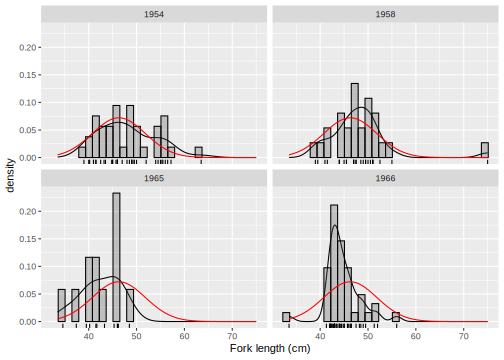
\includegraphics{Labo_BIO4558_files/figure-latex/ano-2-1.pdf}
\caption{\label{fig:ano-2}Distribution de la longueur des esturgeons par année}
\end{figure}

Il semble que la taille des esturgeons est un peu plus petite après la construction du barrage, mais les données sont très variables et les effets ne sont pas parfaitement clairs. Il y a peut-être des problèmes de normalité avec les échantillons de 1954 et 1966, et il y a probablement des valeurs extrêmes dans les échantillons de 1958 et 1966. On va continuer en testant les conditions d'application de l'ANOVA. Il faut d'abord faire l'analyse et examiner les résidus.

\hypertarget{vuxe9rifier-les-conditions-dapplication-de-lanova-paramuxe9trique}{%
\subsection{Vérifier les conditions d'application de l'ANOVA paramétrique}\label{vuxe9rifier-les-conditions-dapplication-de-lanova-paramuxe9trique}}

L'ANOVA paramétrique a trois conditions principales d'application : 1) les résidus sont normalement distribués, 2) la variance des résidus est égale dans tous les traitements (homoscédasticité) et 3) les résidus sont indépendants les uns des autres. Ces conditions doivent être remplies avant qu'on puisse se fier aux résultats de l'ANOVA paramétrique.

\begin{itemize}
\tightlist
\item
  Faites une ANOVA à un critère de classification sur fklngth par année et produisez les graphiques diagnostiques
\end{itemize}

\begin{Shaded}
\begin{Highlighting}[]
\CommentTok{# Fit anova model and plot residual diagnostics}
\NormalTok{anova.model1 <-}\StringTok{ }\KeywordTok{lm}\NormalTok{(fklngth }\OperatorTok{~}\StringTok{ }\NormalTok{year, }\DataTypeTok{data=}\NormalTok{Dam10dat)}
\KeywordTok{par}\NormalTok{(}\DataTypeTok{mfrow =} \KeywordTok{c}\NormalTok{(}\DecValTok{2}\NormalTok{, }\DecValTok{2}\NormalTok{))}
\KeywordTok{plot}\NormalTok{(anova.model1)}
\end{Highlighting}
\end{Shaded}

\begin{figure}
\centering
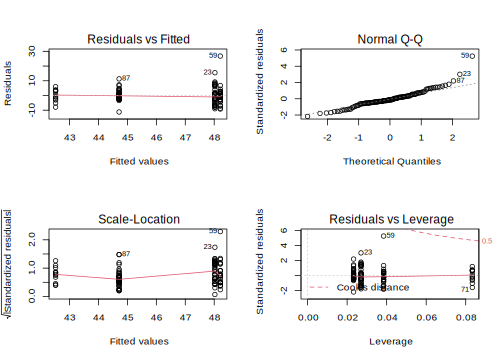
\includegraphics{Labo_BIO4558_files/figure-latex/ano-3-1.pdf}
\caption{\label{fig:ano-3}Conditions d'applications de l'ANOVA}
\end{figure}

D'après les graphiques, on peut douter de la normalité et de l'homogénéité des variances. Notez qu'il y a un point qui ressort vraiment avec une forte valeur résiduelle (cas numéro 59) et qu'il ne s'aligne pas bien avec les autres valeurs: c'est la valeur extrême qui avait été détectée plus tôt. Ce point fera sans doute gonfler la variance résiduelle du groupe auquel il appartient.

Des tests formels nous confirmeront ou infirmeront nos conclusions faites à partir de ces graphiques.

\begin{itemize}
\tightlist
\item
  Faites un test de normalité sur les résidus de l'ANOVA.
\end{itemize}

\begin{Shaded}
\begin{Highlighting}[]
\KeywordTok{shapiro.test}\NormalTok{(}\KeywordTok{residuals}\NormalTok{(anova.model1))}
\end{Highlighting}
\end{Shaded}

\begin{verbatim}
## 
## 	Shapiro-Wilk normality test
## 
## data:  residuals(anova.model1)
## W = 0.91571, p-value = 1.63e-06
\end{verbatim}

Ce test confirme nos soupçons: les résidus ne sont pas distribués normalement. Il faut cependant garder à l'esprit que la puissance est grande et que même de petites déviations de la normalité sont suffisantes pour rejeter l'hypothèse nulle.

\begin{itemize}
\tightlist
\item
  Ensuite, éprouvez l'hypothèse d'égalité des variances (homoscedasticité):
\end{itemize}

\begin{Shaded}
\begin{Highlighting}[]
\KeywordTok{leveneTest}\NormalTok{(fklngth }\OperatorTok{~}\StringTok{ }\NormalTok{year, }\DataTypeTok{data=}\NormalTok{Dam10dat)}
\end{Highlighting}
\end{Shaded}

\begin{verbatim}
## Levene's Test for Homogeneity of Variance (center = median)
##        Df F value  Pr(>F)  
## group   3  2.8159 0.04234 *
##       114                  
## ---
## Signif. codes:  0 '***' 0.001 '**' 0.01 '*' 0.05 '.' 0.1 ' ' 1
\end{verbatim}

La valeur de p vous dit que vous pouvez rejeter l'hypothèse nulle qu'il n'y a aucune différence dans les variances entre les années. Alors, nous concluons que les variances ne sont pas homogènes.

\hypertarget{faire-lanova}{%
\subsection{Faire l'ANOVA}\label{faire-lanova}}

\begin{itemize}
\tightlist
\item
  Faites une ANOVA de fklnght en choisissant / en présumant pour l'instant que les conditions d'application sont suffisamment remplies. Que concluez-vous?
\end{itemize}

\begin{Shaded}
\begin{Highlighting}[]
\KeywordTok{summary}\NormalTok{(anova.model1)}
\end{Highlighting}
\end{Shaded}

\begin{verbatim}
## 
## Call:
## lm(formula = fklngth ~ year, data = Dam10dat)
## 
## Residuals:
##      Min       1Q   Median       3Q      Max 
## -11.2116  -2.6866  -0.7116   2.2103  26.7885 
## 
## Coefficients:
##             Estimate Std. Error t value Pr(>|t|)    
## (Intercept)  48.0243     0.8566  56.061  < 2e-16 ***
## year1958      0.1872     1.3335   0.140  0.88859    
## year1965     -5.5077     1.7310  -3.182  0.00189 ** 
## year1966     -3.3127     1.1684  -2.835  0.00542 ** 
## ---
## Signif. codes:  0 '***' 0.001 '**' 0.01 '*' 0.05 '.' 0.1 ' ' 1
## 
## Residual standard error: 5.211 on 114 degrees of freedom
## Multiple R-squared:  0.1355,	Adjusted R-squared:  0.1128 
## F-statistic: 5.957 on 3 and 114 DF,  p-value: 0.0008246
\end{verbatim}

\begin{enumerate}
\def\labelenumi{\arabic{enumi}.}
\tightlist
\item
  Les 4 coefficients peuvent être utilisés pour obtenir les valeurs prédites par le modèle (i.e.~les moyennes de chaque groupe). La fklngth moyenne de la première année (1954) est 48.0243. Les coefficients pour les 3 autres années sont la différence entre la moyenne de l'année en question et la moyenne de 1954. La moyenne pour 1965 est 48.0243-5.5077=42.5166. Pour chaque coefficient, on a également accès à l'erreur-type, une valeur de t et la probabilité qui lui est associée (H0 que le coefficient est 0). Les poissons étaient plus petits après la construction du barrage qu'en 1954. Vous devez prendre ces p-valeurs avec un grain de sel, car elles ne sont pas corrigées pour les comparaisons multiples et. En général, je porte peu d'attention à cette partie des résultats imprimés et me concentre sur ce qui suit.
\item
  La racine carrée de la variance des résidus (valeurs observées moins valeurs prédites) qui correspond à la variabilité inexpliquée par le modèle (variation de la taille des poissons capturés la même année).
\item
  Le R-carré est la proportion de la variabilité de la variable dépendante qui peut être expliquée par le modèle. Ici, le modèle explique 13.5\% de la variabilité. Les différences de taille d'une année à l'autre sont relativement petites lorsqu'on les compare à la variation de taille entre les poissons capturés la même année.
\item
  La p-valeur associée au test ``omnibus'' que toutes les moyennes sont égales. Ici, p est beaucoup plus petit que 0.05 et on rejetterait H0 pour conclure que fklngth varie selon les années.
\end{enumerate}

La commande \texttt{anova()} produit le tableau d'ANOVA standard qui contient la plupart de cette information:

\begin{Shaded}
\begin{Highlighting}[]
\KeywordTok{anova}\NormalTok{(anova.model1)}
\end{Highlighting}
\end{Shaded}

\begin{verbatim}
## Analysis of Variance Table
## 
## Response: fklngth
##            Df  Sum Sq Mean Sq F value    Pr(>F)    
## year        3  485.26 161.755  5.9574 0.0008246 ***
## Residuals 114 3095.30  27.152                      
## ---
## Signif. codes:  0 '***' 0.001 '**' 0.01 '*' 0.05 '.' 0.1 ' ' 1
\end{verbatim}

La variabilité totale de \texttt{fklngth}, mesurée par la somme des carrés des écarts (Sum sq) est partitionnée en ce qui peut être expliqué par l'année (485.26) et la variabilité résiduelle inexpliquée (3095.30). L'année explique bien (485.26/(3095.30+485.26)=.1355 or 13.55\% de la variabilité). Le carré moyen des résidus (Residual Mean Sq) est leur variance.

\hypertarget{les-comparaisons-multiples}{%
\subsection{Les comparaisons multiples}\label{les-comparaisons-multiples}}

\begin{itemize}
\tightlist
\item
  La fonction \texttt{pairwise.t.test()} peut être utilisée pour comparer des moyennes et ajuster (ou non, si désiré) les probabilités pour le nombre de comparaisons en utilisant l'une des options pour p.adj:
\end{itemize}

Compare toutes les moyennes sans ajuster les probabilités

\begin{Shaded}
\begin{Highlighting}[]
\KeywordTok{pairwise.t.test}\NormalTok{(Dam10dat}\OperatorTok{$}\NormalTok{fklngth, Dam10dat}\OperatorTok{$}\NormalTok{year,}
  \DataTypeTok{p.adj =} \StringTok{"none"}\NormalTok{)}
\end{Highlighting}
\end{Shaded}

\begin{verbatim}
## 
## 	Pairwise comparisons using t tests with pooled SD 
## 
## data:  Dam10dat$fklngth and Dam10dat$year 
## 
##      1954   1958   1965  
## 1958 0.8886 -      -     
## 1965 0.0019 0.0022 -     
## 1966 0.0054 0.0079 0.1996
## 
## P value adjustment method: none
\end{verbatim}

Option \texttt{bonf} ajuste les p-valeurs avec la correction de Bonferroni. Ici, il y a 6 p-valeurs calculées, et la correction de Bonferroni revient à simplement multiplier la p-valeur par 6 (sauf si le résultat est supérieur à 1. Si tel est le cas, la p-valeur ajustée est 1).

\begin{Shaded}
\begin{Highlighting}[]
\KeywordTok{pairwise.t.test}\NormalTok{(Dam10dat}\OperatorTok{$}\NormalTok{fklngth, Dam10dat}\OperatorTok{$}\NormalTok{year,}
  \DataTypeTok{p.adj =} \StringTok{"bonf"}\NormalTok{)}
\end{Highlighting}
\end{Shaded}

\begin{verbatim}
## 
## 	Pairwise comparisons using t tests with pooled SD 
## 
## data:  Dam10dat$fklngth and Dam10dat$year 
## 
##      1954  1958  1965 
## 1958 1.000 -     -    
## 1965 0.011 0.013 -    
## 1966 0.033 0.047 1.000
## 
## P value adjustment method: bonferroni
\end{verbatim}

Option ``holm'' is est la correction séquentielle de Bonferroni dans laquelle les p-valeurs sont ordonnées de (i=1) la plus faible à (N) la plus grande. La correction pour les p-valeurs est (N-i+1). Ici, il y a N=6 paires de moyennes qui sont comparées. La plus petite valeur de p non corrigée est 0.0019 pour 1954 vs 1965. La p-valeur corrigée est donc \(0.0019*(6-1+1)=0.011\). La seconde plus petite p-valeur est 0.0022. Sa p-valeur corrigée est 0.0022*(6-2+1)=0.011. Pour la p- valeur la plus élevée, la correction est (N-N+1)=1, donc la p-valeur corrigée est égale à la p-valeur brute.

\begin{Shaded}
\begin{Highlighting}[]
\KeywordTok{pairwise.t.test}\NormalTok{(Dam10dat}\OperatorTok{$}\NormalTok{fklngth, Dam10dat}\OperatorTok{$}\NormalTok{year,}
  \DataTypeTok{p.adj =} \StringTok{"holm"}\NormalTok{)}
\end{Highlighting}
\end{Shaded}

\begin{verbatim}
## 
## 	Pairwise comparisons using t tests with pooled SD 
## 
## data:  Dam10dat$fklngth and Dam10dat$year 
## 
##      1954  1958  1965 
## 1958 0.889 -     -    
## 1965 0.011 0.011 -    
## 1966 0.022 0.024 0.399
## 
## P value adjustment method: holm
\end{verbatim}

L'option ``fdr'' sert à contrôler le ``false discovery rate''.

\begin{Shaded}
\begin{Highlighting}[]
\KeywordTok{pairwise.t.test}\NormalTok{(Dam10dat}\OperatorTok{$}\NormalTok{fklngth, Dam10dat}\OperatorTok{$}\NormalTok{year,}
  \DataTypeTok{p.adj =} \StringTok{"fdr"}\NormalTok{)}
\end{Highlighting}
\end{Shaded}

\begin{verbatim}
## 
## 	Pairwise comparisons using t tests with pooled SD 
## 
## data:  Dam10dat$fklngth and Dam10dat$year 
## 
##      1954   1958   1965  
## 1958 0.8886 -      -     
## 1965 0.0066 0.0066 -     
## 1966 0.0108 0.0119 0.2395
## 
## P value adjustment method: fdr
\end{verbatim}

Les quatre méthodes mènent ici à la même conclusion: les poissons sont plus gros après la construction du barrage et toutes les comparaisons entre les années 50 et 60 sont significatives alors que les différences entre 54 et 58 ou 65 et 66 ne le sont pas. La conclusion ne dépend pas du choix de méthode.

Dans d'autres situations, vous pourriez obtenir des résultats contradictoires. Alors, quelle méthode choisir? Les p-valeurs qui ne sont pas corrigées sont certainement suspectes lorsqu'il y a plusieurs comparaisons. D'un autre coté, la correction de Bonferroni est conservatrice et le devient encore plus lorsqu'il y a de très nombreuses comparaisons. Des travaux récents suggèrent que la correction fdr est un bon compromis lorsqu'il y a beaucoup de comparaisons.

La méthode de Tukey est l'une des plus populaires et est facile à utiliser en R (notez cependant qu'il y a une sale petit bogue qui se manifeste quand la variable indépendante peut ressemble à un nombre plutôt qu'un facteur, ce qui explique la petite pirouette avec paste dans mon code):

\begin{Shaded}
\begin{Highlighting}[]
\NormalTok{Dam10dat}\OperatorTok{$}\NormalTok{myyear <-}\StringTok{ }\KeywordTok{as.factor}\NormalTok{(}\KeywordTok{paste}\NormalTok{(}\StringTok{""}\NormalTok{, Dam10dat}\OperatorTok{$}\NormalTok{year))}
\KeywordTok{TukeyHSD}\NormalTok{(}\KeywordTok{aov}\NormalTok{(fklngth }\OperatorTok{~}\StringTok{ }\NormalTok{myyear, }\DataTypeTok{data =}\NormalTok{ Dam10dat))}
\end{Highlighting}
\end{Shaded}

\begin{verbatim}
##   Tukey multiple comparisons of means
##     95% family-wise confidence level
## 
## Fit: aov(formula = fklngth ~ myyear, data = Dam10dat)
## 
## $myyear
##                   diff        lwr        upr     p adj
##  1958- 1954  0.1872141  -3.289570  3.6639986 0.9990071
##  1965- 1954 -5.5076577 -10.021034 -0.9942809 0.0100528
##  1966- 1954 -3.3126964  -6.359223 -0.2661701 0.0274077
##  1965- 1958 -5.6948718 -10.436304 -0.9534397 0.0116943
##  1966- 1958 -3.4999106  -6.875104 -0.1247171 0.0390011
##  1966- 1965  2.1949612  -2.240630  6.6305526 0.5710111
\end{verbatim}

\begin{Shaded}
\begin{Highlighting}[]
\KeywordTok{plot}\NormalTok{(}\KeywordTok{TukeyHSD}\NormalTok{(}\KeywordTok{aov}\NormalTok{(fklngth }\OperatorTok{~}\StringTok{ }\NormalTok{myyear, }\DataTypeTok{data =}\NormalTok{ Dam10dat)))}
\end{Highlighting}
\end{Shaded}

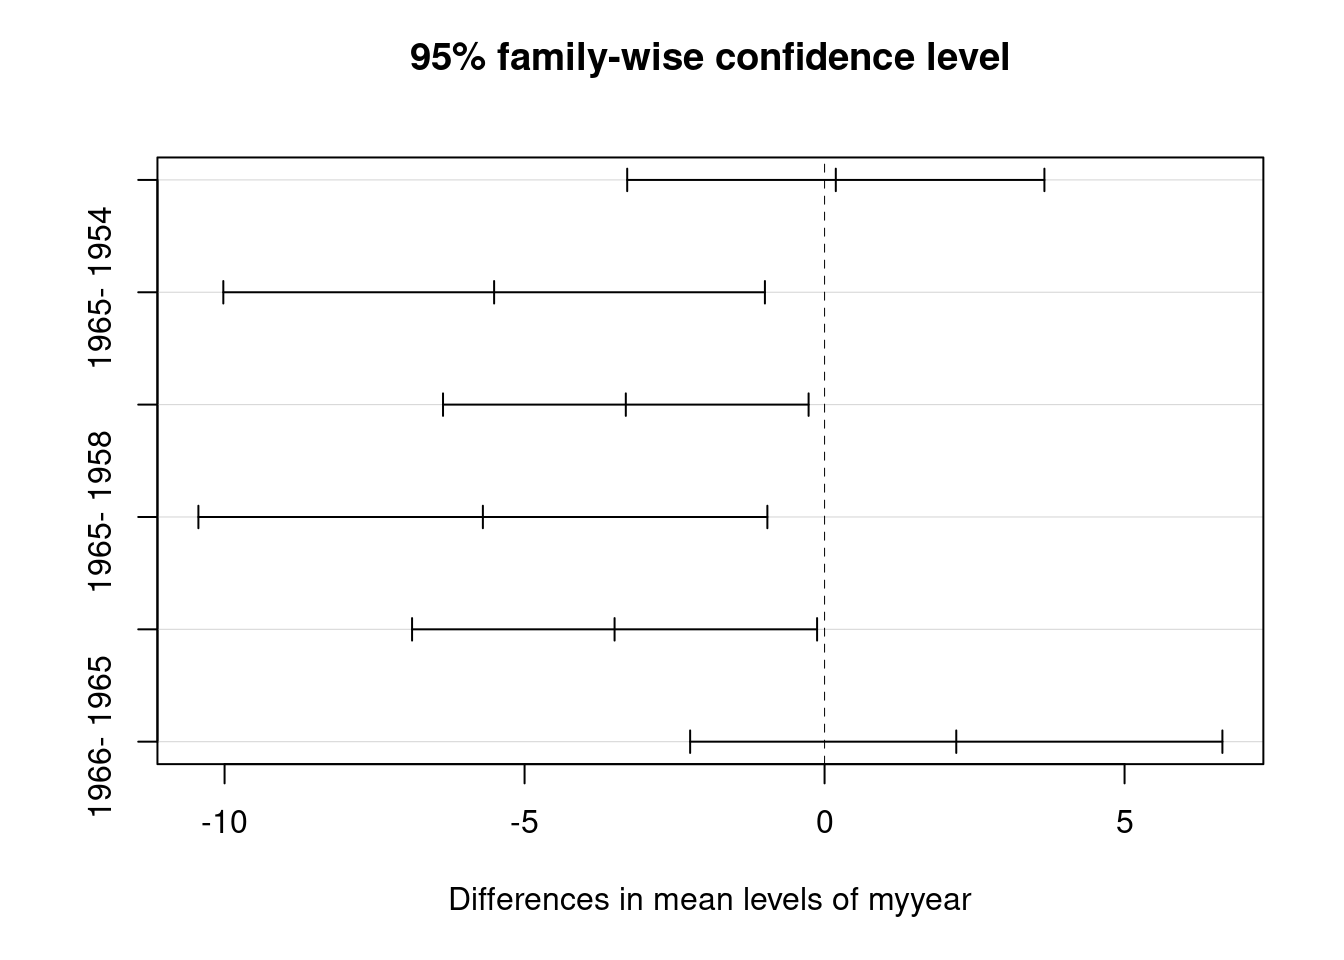
\includegraphics{Labo_BIO4558_files/figure-latex/ano-13-1.pdf}
Les intervalles de confiance, corrigés pour les comparaisons multiples par la méthode de Tukey, sont illustrés pour les différences entre années. Malheureusement les légendes ne sont pas complètes, mais l'ordre est le même que dans le tableau précédent.

Le package multcomp peut produire de meilleurs graphiques, mais requiert un peu plus de code:

\begin{Shaded}
\begin{Highlighting}[]
\CommentTok{# Alternative way to compute Tukey multiple comparisons}
\CommentTok{# set up a one-way ANOVA}
\NormalTok{anova.fkl.vs.year <-}\StringTok{ }\KeywordTok{aov}\NormalTok{(}\KeywordTok{aov}\NormalTok{(fklngth }\OperatorTok{~}\StringTok{ }\NormalTok{myyear, }\DataTypeTok{data =}\NormalTok{ Dam10dat))}
\CommentTok{# set up all-pairs comparisons for factor `year'}

\NormalTok{meandiff <-}\StringTok{ }\KeywordTok{glht}\NormalTok{(anova.fkl.vs.year, }\DataTypeTok{linfct =} \KeywordTok{mcp}\NormalTok{(}\DataTypeTok{myyear =}
\StringTok{"Tukey"}\NormalTok{))}
\KeywordTok{confint}\NormalTok{(meandiff)}
\end{Highlighting}
\end{Shaded}

\begin{verbatim}
## 
## 	 Simultaneous Confidence Intervals
## 
## Multiple Comparisons of Means: Tukey Contrasts
## 
## 
## Fit: aov(formula = aov(fklngth ~ myyear, data = Dam10dat))
## 
## Quantile = 2.5955
## 95% family-wise confidence level
##  
## 
## Linear Hypotheses:
##                    Estimate lwr      upr     
##  1958 -  1954 == 0   0.1872  -3.2738   3.6482
##  1965 -  1954 == 0  -5.5077 -10.0006  -1.0148
##  1966 -  1954 == 0  -3.3127  -6.3454  -0.2800
##  1965 -  1958 == 0  -5.6949 -10.4148  -0.9749
##  1966 -  1958 == 0  -3.4999  -6.8598  -0.1400
##  1966 -  1965 == 0   2.1950  -2.2205   6.6104
\end{verbatim}

\begin{Shaded}
\begin{Highlighting}[]
\NormalTok{old.par <-}\StringTok{ }\KeywordTok{par}\NormalTok{(}\DataTypeTok{mai =} \KeywordTok{c}\NormalTok{(}\DecValTok{1}\NormalTok{, }\FloatTok{1.25}\NormalTok{, }\DecValTok{1}\NormalTok{, }\DecValTok{1}\NormalTok{))}
\KeywordTok{plot}\NormalTok{(meandiff)}
\end{Highlighting}
\end{Shaded}

\begin{figure}
\centering
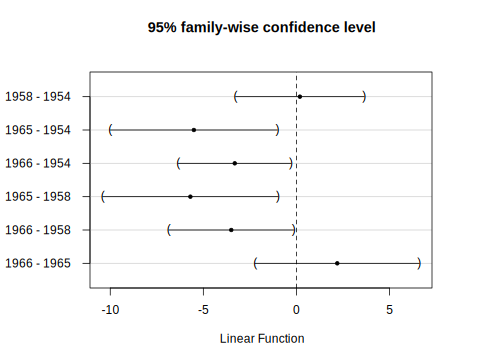
\includegraphics{Labo_BIO4558_files/figure-latex/ano-14-1.pdf}
\caption{\label{fig:ano-14}Différence anuelles dans la longueur des esturgeons}
\end{figure}

\begin{Shaded}
\begin{Highlighting}[]
\KeywordTok{par}\NormalTok{(old.par)}
\end{Highlighting}
\end{Shaded}

C'est un peu mieux, mais ce qui le serait encore plus c'est un graphique des moyennes, avec leurs intervalles de confiance ajustés pour les comparaisons multiples:

\begin{Shaded}
\begin{Highlighting}[]
\CommentTok{# Compute and plot means and Tukey CI}
\NormalTok{means <-}\StringTok{ }\KeywordTok{glht}\NormalTok{(anova.fkl.vs.year, }\DataTypeTok{linfct =} \KeywordTok{mcp}\NormalTok{(}\DataTypeTok{myyear =}
\StringTok{"Tukey"}\NormalTok{))}
\NormalTok{cimeans <-}\StringTok{ }\KeywordTok{cld}\NormalTok{(means)}
\CommentTok{# use sufficiently large upper margin}
\NormalTok{old.par <-}\StringTok{ }\KeywordTok{par}\NormalTok{(}\DataTypeTok{mai =} \KeywordTok{c}\NormalTok{(}\DecValTok{1}\NormalTok{, }\DecValTok{1}\NormalTok{, }\FloatTok{1.25}\NormalTok{, }\DecValTok{1}\NormalTok{))}
\CommentTok{# plot}
\KeywordTok{plot}\NormalTok{(cimeans)}
\end{Highlighting}
\end{Shaded}

\begin{figure}
\centering
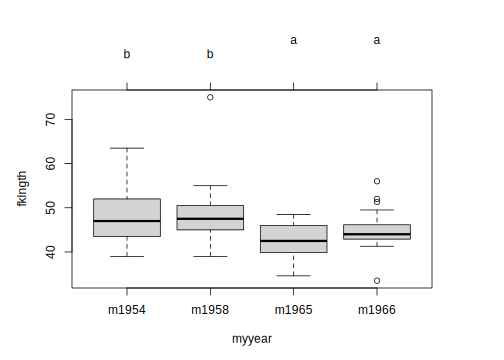
\includegraphics{Labo_BIO4558_files/figure-latex/ano-15-1.pdf}
\caption{\label{fig:ano-15}Différence anuelles dans la longueur des esturgeons}
\end{figure}

\begin{Shaded}
\begin{Highlighting}[]
\KeywordTok{par}\NormalTok{(old.par)}
\end{Highlighting}
\end{Shaded}

Notez les lettres au dessus du graphique: les années étiquetées avec la même lettre ne diffèrent pas significativement l'une de l'autre.

\hypertarget{transformations-de-donnuxe9es-et-anova-non-paramuxe9trique}{%
\section{Transformations de données et ANOVA non-paramétrique}\label{transformations-de-donnuxe9es-et-anova-non-paramuxe9trique}}

Dans l'exemple précédent sur les différences annuelles de la variable fklgnth, on a noté que les conditions d'application de l'ANOVA n'étaient pas remplies. Si les données ne remplissent pas les conditions de l'ANOVA paramétrique, il y a 3 options : 1) Ne rien faire. Si les effectifs dans chaque groupe sont grands, on peut relaxer les conditions d'application car l'ANOVA est alors assez robuste aux violations de normalité (mais moins aux violations d'homoscedasticité), 2) on peut transformer les données, ou 3) on peut faire une analyse non-paramétrique.

\begin{itemize}
\tightlist
\item
  Refaites l'ANOVA de la section précédente après avoir transformé en faisant le logarithme à la base de 10. Avec les données transformées, est-ce que les problèmes qui avaient été identifiés dis- paraissent ?
\end{itemize}

\begin{Shaded}
\begin{Highlighting}[]
\CommentTok{# Fit anova model on log10 of fklngth and plot residual diagnostics}
\KeywordTok{par}\NormalTok{(}\DataTypeTok{mfrow =} \KeywordTok{c}\NormalTok{(}\DecValTok{2}\NormalTok{, }\DecValTok{2}\NormalTok{))}
\NormalTok{anova.model2 <-}\StringTok{ }\KeywordTok{lm}\NormalTok{(}\KeywordTok{log10}\NormalTok{(fklngth) }\OperatorTok{~}\StringTok{ }\NormalTok{year, }\DataTypeTok{data=}\NormalTok{Dam10dat)}
\KeywordTok{plot}\NormalTok{(anova.model2)}
\end{Highlighting}
\end{Shaded}

\begin{figure}
\centering
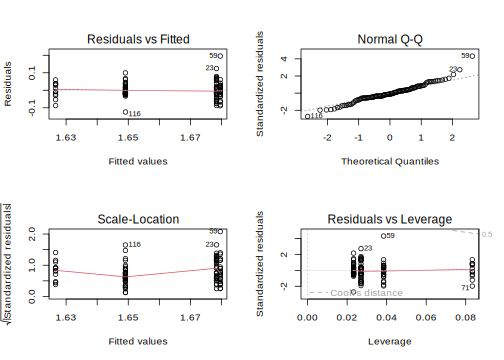
\includegraphics{Labo_BIO4558_files/figure-latex/ano-16-1.pdf}
\caption{\label{fig:ano-16}Conditions d'application de l'ANOVA}
\end{figure}

Les graphiques diagnostiques des résidus donnent:

Les graphiques sont à peine mieux ici. Si on fait le test Wilk-Shapiro sur les résidus, on obtient:

\begin{Shaded}
\begin{Highlighting}[]
\KeywordTok{shapiro.test}\NormalTok{(}\KeywordTok{residuals}\NormalTok{(anova.model2))}
\end{Highlighting}
\end{Shaded}

\begin{verbatim}
## 
## 	Shapiro-Wilk normality test
## 
## data:  residuals(anova.model2)
## W = 0.96199, p-value = 0.002048
\end{verbatim}

Alors, on a toujours des problèmes avec la normalité et on est juste sur le seuil de décision pour l'égalité des variances. Vous avez le choix à ce point: 1) essayer de trouver une autre transformation pour mieux rencontrer les conditions d'application, 2) assumer que les données sont rencontrent suffisamment les conditions d'application, ou 3) faire une ANOVA non-paramétrique.

\begin{itemize}
\tightlist
\item
  L'analogue non-paramétrique de l'ANOVA à un critère de classifica-
  tion le plus employé est le test de Kruskall-Wallis. Faites ce test sur \texttt{fklngth} et comparez les résultats à ceux de l'analyse paramétrique. Que concluez-vous?
\end{itemize}

\begin{Shaded}
\begin{Highlighting}[]
\KeywordTok{kruskal.test}\NormalTok{(fklngth }\OperatorTok{~}\StringTok{ }\NormalTok{year, }\DataTypeTok{data=}\NormalTok{Dam10dat)}
\end{Highlighting}
\end{Shaded}

\begin{verbatim}
## 
## 	Kruskal-Wallis rank sum test
## 
## data:  fklngth by year
## Kruskal-Wallis chi-squared = 15.731, df = 3, p-value = 0.001288
\end{verbatim}

La conclusion est donc la même qu'avec l'ANOVA paramétrique: on rejette l'hypothèse nulle que le rang moyen est le même pour chaque année. Donc, même si les conditions d'application de l'analyse paramétrique n'étaient pas parfaitement rencontrées, les conclusions sont les mêmes, ce qui illustre la robustesse de l'ANOVA paramétrique.

\hypertarget{examen-des-valeurs-extruxeames}{%
\section{Examen des valeurs extrêmes}\label{examen-des-valeurs-extruxeames}}

Vous devriez avoir remarqué au cours des analyses précédentes qu'il y avait peut-être des valeurs extrêmes dans les données. Ces points étaient évidents dans le Box Plot de fklngth by year et ont été notés comme les points 59, 23, et 87 dans les diagrammes de probabilité des résidus et dans le diagramme de dispersion des résidus et des valeurs estimées. En général, vous devez avoir de très bonnes raisons pour enlever des valeurs extrêmes de la base de données (i.e.~vous savez qu'il y a eu une erreur avec un cas). Cependant, il est quand même toujours valable de voir comment l'analyse change en enlevant des valeurs extrêmes de la base de données.

\begin{itemize}
\tightlist
\item
  Répétez l'ANOVA originale sur fklngth et year mais faites le avec un sous-ensemble de données sans les valeurs extrêmes. Est-ce que les conclusions ont changé?
\end{itemize}

\begin{Shaded}
\begin{Highlighting}[]
\NormalTok{Damsubset<-Dam10dat[}\OperatorTok{-}\KeywordTok{c}\NormalTok{(}\DecValTok{23}\NormalTok{,}\DecValTok{59}\NormalTok{,}\DecValTok{87}\NormalTok{),] }\CommentTok{#removes obs 23, 59 and 87}
\NormalTok{aov.Damsubset <-}\StringTok{ }\KeywordTok{aov}\NormalTok{(fklngth }\OperatorTok{~}\StringTok{ }\KeywordTok{as.factor}\NormalTok{(year), Damsubset)}
\KeywordTok{summary}\NormalTok{(aov.Damsubset)}
\end{Highlighting}
\end{Shaded}

\begin{verbatim}
##                  Df Sum Sq Mean Sq F value   Pr(>F)    
## as.factor(year)   3  367.5  122.50   6.894 0.000267 ***
## Residuals       111 1972.4   17.77                     
## ---
## Signif. codes:  0 '***' 0.001 '**' 0.01 '*' 0.05 '.' 0.1 ' ' 1
\end{verbatim}

\begin{Shaded}
\begin{Highlighting}[]
\KeywordTok{shapiro.test}\NormalTok{(}\KeywordTok{residuals}\NormalTok{(aov.Damsubset))}
\end{Highlighting}
\end{Shaded}

\begin{verbatim}
## 
## 	Shapiro-Wilk normality test
## 
## data:  residuals(aov.Damsubset)
## W = 0.98533, p-value = 0.2448
\end{verbatim}

\begin{Shaded}
\begin{Highlighting}[]
\KeywordTok{leveneTest}\NormalTok{(fklngth }\OperatorTok{~}\StringTok{ }\NormalTok{year, Damsubset)}
\end{Highlighting}
\end{Shaded}

\begin{verbatim}
## Levene's Test for Homogeneity of Variance (center = median)
##        Df F value   Pr(>F)   
## group   3  4.6237 0.004367 **
##       111                    
## ---
## Signif. codes:  0 '***' 0.001 '**' 0.01 '*' 0.05 '.' 0.1 ' ' 1
\end{verbatim}

L'élimination de trois valeurs extrêmes améliore un peu les choses, mais ce n'est pas parfait. On a toujours une problème avec les variances, mais les résidus sont maintenant normaux. Cependant, le fait que la conclusion qu'on tire de l'ANOVA originale ne change pas en enlevant les points renforce le fait qu'on n'a pas une bonne raison pour enlever les points.

Commandes R pour refaire l'ANOVA sur le sous-ensemble de données

\begin{Shaded}
\begin{Highlighting}[]
\NormalTok{Damsubset<-Dam10dat[}\OperatorTok{-}\KeywordTok{c}\NormalTok{(}\DecValTok{23}\NormalTok{,}\DecValTok{59}\NormalTok{,}\DecValTok{87}\NormalTok{),]}
\CommentTok{# removes obs 23, 59 and 87}
\NormalTok{aov.Damsubset <-}\StringTok{ }\KeywordTok{aov}\NormalTok{(fklngth }\OperatorTok{~}\StringTok{ }\KeywordTok{as.factor}\NormalTok{(year), Damsubset)}
\KeywordTok{summary}\NormalTok{(aov.Damsubset)}
\KeywordTok{shapiro.test}\NormalTok{(}\KeywordTok{residuals}\NormalTok{(aov.Damsubset))}
\KeywordTok{leveneTest}\NormalTok{(fklngth }\OperatorTok{~}\StringTok{ }\NormalTok{year, Damsubset)}
\end{Highlighting}
\end{Shaded}

\hypertarget{test-de-permutation}{%
\section{Test de permutation}\label{test-de-permutation}}

Commande R pour un test de permutation d'une ANOVA à un critère de classification.

\begin{Shaded}
\begin{Highlighting}[]
\CommentTok{#############################################################}
\CommentTok{# Permutation Test for one-way ANOVA}
\CommentTok{# modified from code written by David C. Howell}
\CommentTok{# http://www.uvm.edu/~dhowell/StatPages/More_Stuff/Permutation%20Anova/PermTestsAnova.html}
\CommentTok{# set desired number of permutations}
\NormalTok{nreps <-}\DecValTok{500}
\CommentTok{# to simplify reuse of this code, copy desired dataframe to mydata}
\NormalTok{mydata<-Dam10dat}
\CommentTok{# copy model formula to myformula}
\NormalTok{myformula<-}\KeywordTok{as.formula}\NormalTok{(}\StringTok{"fklngth ~ year"}\NormalTok{)}
\CommentTok{# copy dependent variable vector to mydep}
\NormalTok{mydep<-mydata}\OperatorTok{$}\NormalTok{fklngth}
\CommentTok{# copy independent variable vector to myindep}
\NormalTok{myindep<-}\KeywordTok{as.factor}\NormalTok{(mydata}\OperatorTok{$}\NormalTok{year)}
\CommentTok{################################################}
\CommentTok{# You should not need to modify code chunk below}
\CommentTok{################################################}
\CommentTok{# Compute observed F value for original sample}
\NormalTok{mod1 <-}\StringTok{ }\KeywordTok{lm}\NormalTok{(myformula, }\DataTypeTok{data=}\NormalTok{mydata) }\CommentTok{# Standard Anova}
\NormalTok{ANOVA <-}\StringTok{ }\KeywordTok{summary}\NormalTok{(}\KeywordTok{aov}\NormalTok{(mod1)) }\CommentTok{# Save summary to variable}
\NormalTok{observedF<-}\StringTok{ }\NormalTok{ANOVA[[}\DecValTok{1}\NormalTok{]]}\OperatorTok{$}\StringTok{"F value"}\NormalTok{[}\DecValTok{1}\NormalTok{] }\CommentTok{# Save observed F value}
\CommentTok{# Print standard ANOVA results}
\KeywordTok{cat}\NormalTok{(}\StringTok{" The standard ANOVA for these data follows "}\NormalTok{,}
\StringTok{"}\CharTok{\textbackslash{}n}\StringTok{"}\NormalTok{)}
\KeywordTok{print}\NormalTok{(ANOVA, }\StringTok{"}\CharTok{\textbackslash{}n}\StringTok{"}\NormalTok{)}
\KeywordTok{cat}\NormalTok{(}\StringTok{"}\CharTok{\textbackslash{}n}\StringTok{"}\NormalTok{)}
\KeywordTok{cat}\NormalTok{(}\StringTok{"}\CharTok{\textbackslash{}n}\StringTok{"}\NormalTok{)}
\KeywordTok{print}\NormalTok{(}\StringTok{"Resampling as in Manly with unrestricted sampling of obser-}
\StringTok{vations. "}\NormalTok{)}
\CommentTok{# Now start resampling}
\NormalTok{Fboot <-}\StringTok{ }\KeywordTok{numeric}\NormalTok{(nreps) }\CommentTok{# initalize vector to receive permuted}
\NormalTok{values}
\NormalTok{Fboot[}\DecValTok{1}\NormalTok{] <-}\StringTok{ }\NormalTok{observedF}
\ControlFlowTok{for}\NormalTok{ (i }\ControlFlowTok{in} \DecValTok{2}\OperatorTok{:}\NormalTok{nreps) \{}
\NormalTok{newdependent <-}\StringTok{ }\KeywordTok{sample}\NormalTok{(mydep, }\KeywordTok{length}\NormalTok{(mydep)) }\CommentTok{# randomize dep}
\NormalTok{var}
\NormalTok{mod2 <-}\StringTok{ }\KeywordTok{lm}\NormalTok{(newdependent }\OperatorTok{~}\StringTok{ }\NormalTok{myindep) }\CommentTok{# refit model}
\NormalTok{b <-}\StringTok{ }\KeywordTok{summary}\NormalTok{(}\KeywordTok{aov}\NormalTok{(mod2))}
\NormalTok{Fboot[i] <-}\StringTok{ }\NormalTok{b[[}\DecValTok{1}\NormalTok{]]}\OperatorTok{$}\StringTok{"F value"}\NormalTok{[}\DecValTok{1}\NormalTok{] }\CommentTok{# store F stats}
\NormalTok{\}}
\NormalTok{permprob <-}\StringTok{ }\KeywordTok{length}\NormalTok{(Fboot[Fboot }\OperatorTok{>=}\StringTok{ }\NormalTok{observedF])}\OperatorTok{/}\NormalTok{nreps}
\KeywordTok{cat}\NormalTok{(}\StringTok{" The permutation probability value is: "}\NormalTok{, permprob,}
\StringTok{"}\CharTok{\textbackslash{}n}\StringTok{"}\NormalTok{)}
\CommentTok{# end of code chunk for permutation}
\end{Highlighting}
\end{Shaded}

Version lmPerm du test de permutation.

\begin{Shaded}
\begin{Highlighting}[]
\CommentTok{## lmPerm version of permutation test}
\KeywordTok{require}\NormalTok{(lmPerm2)}
\CommentTok{# for generality, copy desired dataframe to mydata}
\CommentTok{# and model formula to myformula}
\NormalTok{mydata <-}\StringTok{ }\NormalTok{Dam10dat}
\NormalTok{myformula <-}\StringTok{ }\KeywordTok{as.formula}\NormalTok{(}\StringTok{"fklngth ~ year"}\NormalTok{)}
\CommentTok{# Fit desired model on the desired dataframe}
\NormalTok{mymodel <-}\StringTok{ }\KeywordTok{lm}\NormalTok{(myformula, }\DataTypeTok{data =}\NormalTok{ mydata)}
\CommentTok{# Calculate permutation p-value}
\KeywordTok{anova}\NormalTok{(}\KeywordTok{lmp}\NormalTok{(myformula, }\DataTypeTok{data =}\NormalTok{ mydata, }\DataTypeTok{perm =} \StringTok{"Prob"}\NormalTok{, }\DataTypeTok{center=}\OtherTok{FALSE}\NormalTok{, }\DataTypeTok{Ca=}\FloatTok{0.001}\NormalTok{))}
\end{Highlighting}
\end{Shaded}

\cleardoublepage

\hypertarget{appendix-appendice}{%
\appendix \addcontentsline{toc}{chapter}{\appendixname}}


\hypertarget{petit-guide-pour-rmarkdown}{%
\chapter{Petit guide pour Rmarkdown}\label{petit-guide-pour-rmarkdown}}

\hypertarget{syntaxe-markdown}{%
\section{Syntaxe Markdown}\label{syntaxe-markdown}}

Ceci est un petit document qui résume la syntaxe de Markdown

On utilise \# (6 max.) pour créer des titres (section) :

\texttt{\#\#\#\ Titre\ 3}

\texttt{\#\#\#\#\ Titre\ 4}

\texttt{\#\#\#\#\ Titre\ 5}

\texttt{\#\#\#\#\#\ Titre\ 6}

Donne

\hypertarget{titre-3}{%
\subsection{Titre 3}\label{titre-3}}

\hypertarget{titre-4}{%
\subsubsection{Titre 4}\label{titre-4}}

\hypertarget{titre-5}{%
\subsubsection{Titre 5}\label{titre-5}}

\hypertarget{titre-6}{%
\paragraph{Titre 6}\label{titre-6}}

On entoure le texte des symboles * ou \_ pour mettre le texte en italique ou en gras.
Un symbole pour mettre en italique:
\texttt{*Texte\ en\ Italique*}
\emph{Texte en Italique}

\texttt{\_Texte\ en\ Italique\_}
\emph{Texte en Italique}

Deux symboles pour mettre en gras:
\texttt{**Texte\ gras**}
\textbf{Texte gras}

\texttt{\_\_Texte\ gras\_\_}
\textbf{Texte gras}

On utilise une combinaison des 2 charactère pour obtenir du \textbf{texte gras et \emph{italique}}.

Pour créer un liste on utilise le symbole \texttt{-} suivit d'une espace.

\begin{itemize}
\tightlist
\item
  Il doit y avoir une ligne vide avant la liste.
\item
  On doit ajouter quelques espaces après chaque ligne.

  \begin{itemize}
  \tightlist
  \item
    Pour ajouter des niveau à la liste on indente (tab) 2 fois, puis on ajoute le symbole + suivit d'un espace.
  \item
    Ici encore, on doit ajouter quelques espaces après chaque lignes.
  \end{itemize}
\item
  Il doit y avoir une ligne vide après la liste.
\end{itemize}

On peut aussi créer des liste avec des numéro ou des lettre.

\begin{enumerate}
\def\labelenumi{\arabic{enumi}.}
\tightlist
\item
  On doit simplement mettre un point après le chiffre ou la lettre, suivit d'un espace

  \begin{enumerate}
  \def\labelenumii{\alph{enumii}.}
  \tightlist
  \item
    Encore une fois, il peut y avoir plusieurs niveaux
    ii). Mais pas plus de 3 niveau
  \end{enumerate}
\end{enumerate}

Pour écrire des équation mathématique, on entoure le texte du symbole \$

\(K = 0.5\)

\(\log(x + k)\)

Pour faire un tableau, on fait comme suit (noter que l'alignement des symbole est sans importance) :

\begin{verbatim}
colonne 1  |colonne 2|colonne 3|colonne 4
---------|--------|--------|-----------
cellulle | cellulle |cellulle| cellulle
cellulle   | cellulle |cellulle| cellulle
cellulle | cellulle |cellulle| cellulle
\end{verbatim}

On peut utiliser le symbole \textgreater{} pour indenter un paragraphe (le résultat est différent entre PDF et HTML) :

\begin{quote}
En HTML, ça produit un résultat étrange \ldots{}
\textgreater{} mais bon \ldots{}
\end{quote}

On peut écrire dans la même police que celle du code en entourant le texte avec le symbole ` :
\texttt{variable}

Si l'on veut utilisé un symbole dans le texte sans qu'il modifie le texte, il faut mettre le symbole \textbackslash{} devant.

Pour inséré un lien, on entoure le texte avec {[} {]}, et on met l'addresse dans des paranthèse () immédiatement à coté:
\href{http://rmarkdown.rstudio.com}{R Markdown}

On peut tracer un ligne horizontale en répétant le symbole - 3 fois ou plus :

\begin{center}\rule{0.5\linewidth}{0.5pt}\end{center}

\hypertarget{uxe0-propos-de-latex}{%
\section{À propos de LaTex}\label{uxe0-propos-de-latex}}

Ce qui suit concerne uniquement ceux qui on installer LaTex.
Les fonction LaTex serve à modifier le texte, mais ne fonctionne que lorsqu'on produit un document PDF (ça fonctionne peut-être aussi pour les document word). Ils en existe beaucoup trop de fonction pour toutes les énumérer ici. Google est votre ami.

Voici quelques exemple:

\begin{Shaded}
\begin{Highlighting}[]
\FunctionTok{\textbackslash{}emph}\NormalTok{\{texte italique\}}
\FunctionTok{\textbackslash{}textcolor}\NormalTok{\{red\}\{texte rouge\}}
\FunctionTok{\textbackslash{}texttt}\NormalTok{\{même police que le code de R\}}
\end{Highlighting}
\end{Shaded}

Le nom de la prochaine fonction est assez descriptif

\begin{Shaded}
\begin{Highlighting}[]
\FunctionTok{\textbackslash{}pagebreak}
\end{Highlighting}
\end{Shaded}

\hypertarget{concernant-le-code-dans-notebook}{%
\section{Concernant le code dans notebook}\label{concernant-le-code-dans-notebook}}

Vous devez écrire le code à l'intérieur de bloc de code, sinon il ne sera pas interpréter comme du code, mais comme du texte.
Vous pouvez taper directement la notation pour créer un bloc code ou utiliser les raccourci clavier de RStudio
Pour créer un nouveau bloc de code, taper \emph{\texttt{\textasciigrave{}\textasciigrave{}\textasciigrave{}\{r\}}} pour ouvrir le bloc et \emph{\texttt{\textasciigrave{}\textasciigrave{}\textasciigrave{}}} pour le fermer.
Sinon, appuyer sur \emph{Ctrl+Alt+I}
Dans Rstudio, pour éxécuter le code à l'intérieur d'un bloc appuyer sur \emph{Ctrl+Shift+Enter} ou cliquer sur le boutton \emph{Run} (dans le bloc, en haut à droite).

Charger les données et les packages dans le premier bloc de code.

\begin{verbatim}
```{r} #ouverture du bloc de code
 code
``` #fermeture du bloc code
\end{verbatim}

Lorsque vous exécuter du code dans un bloc, le résultat apparait directement en dessous de la du bloc (si votre document est un R Notebook).
L'option \texttt{fig.cap} fonctionnement seulement lorsqu'on génère un PDF.

Lorsque vous sauvegarder un notebook, un fichier HTLM contenant le code et les résultats est sauvegarder en même temps. Cliquer sur le bouton \emph{Preview} ou appuyer sur \emph{Ctrl+Shift+K} pour voir le fichier HTML.

\begin{Shaded}
\begin{Highlighting}[]
\BaseNTok{```\{r, fig.cap = "Exemple de graphique tiré du fichier d'aide de la fonction stat_bin"\}}
\BaseNTok{ggplot(diamonds, aes(carat)) +}
\BaseNTok{  geom_histogram()}

\BaseNTok{ggplot(diamonds, aes(carat)) +}
\BaseNTok{  geom_histogram(binwidth = 0.01)}

\BaseNTok{ggplot(diamonds, aes(carat)) +}
\BaseNTok{  geom_histogram(bins = 200)}
\BaseNTok{```}
\end{Highlighting}
\end{Shaded}

\begin{Shaded}
\begin{Highlighting}[]
\KeywordTok{ggplot}\NormalTok{(diamonds, }\KeywordTok{aes}\NormalTok{(carat)) }\OperatorTok{+}
\StringTok{  }\KeywordTok{geom_histogram}\NormalTok{()}
\end{Highlighting}
\end{Shaded}

\begin{verbatim}
## `stat_bin()` using `bins = 30`. Pick better value with `binwidth`.
\end{verbatim}

\begin{figure}
\centering
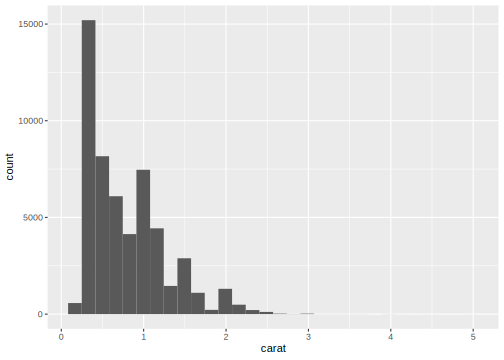
\includegraphics{Labo_BIO4558_files/figure-latex/unnamed-chunk-18-1.pdf}
\caption{\label{fig:unnamed-chunk-18-1}Exemple de graphique tiré du fichier d'aide de la fonction stat\_bin}
\end{figure}

\begin{Shaded}
\begin{Highlighting}[]
\KeywordTok{ggplot}\NormalTok{(diamonds, }\KeywordTok{aes}\NormalTok{(carat)) }\OperatorTok{+}
\StringTok{  }\KeywordTok{geom_histogram}\NormalTok{(}\DataTypeTok{binwidth =} \FloatTok{0.01}\NormalTok{)}
\end{Highlighting}
\end{Shaded}

\begin{figure}
\centering
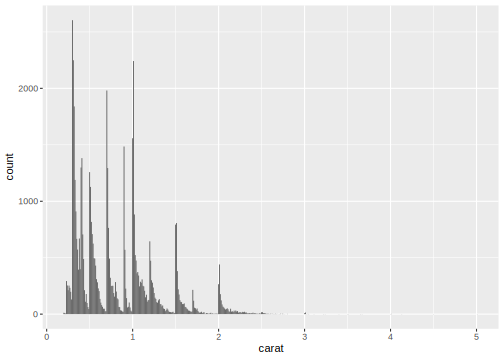
\includegraphics{Labo_BIO4558_files/figure-latex/unnamed-chunk-18-2.pdf}
\caption{\label{fig:unnamed-chunk-18-2}Exemple de graphique tiré du fichier d'aide de la fonction stat\_bin}
\end{figure}

\begin{Shaded}
\begin{Highlighting}[]
\KeywordTok{ggplot}\NormalTok{(diamonds, }\KeywordTok{aes}\NormalTok{(carat)) }\OperatorTok{+}
\StringTok{  }\KeywordTok{geom_histogram}\NormalTok{(}\DataTypeTok{bins =} \DecValTok{200}\NormalTok{)}
\end{Highlighting}
\end{Shaded}

\begin{figure}
\centering
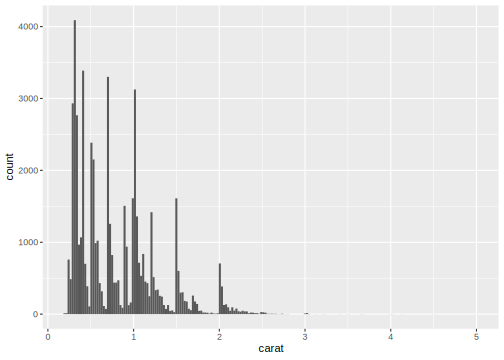
\includegraphics{Labo_BIO4558_files/figure-latex/unnamed-chunk-18-3.pdf}
\caption{\label{fig:unnamed-chunk-18-3}Exemple de graphique tiré du fichier d'aide de la fonction stat\_bin}
\end{figure}

\printindex

\end{document}
